\documentclass[11pt]{article}
\usepackage[T1]{fontenc}
\usepackage[utf8]{inputenc}
\usepackage[margin=1.15in]{geometry}
\usepackage{amsmath,amssymb,amsthm}
\usepackage{mathptmx}
\usepackage{microtype}
\usepackage{fancyvrb}
\usepackage{longtable}
\usepackage{tikz}
\usetikzlibrary{circuits.logic.US,positioning,arrows.meta,calc,fit,backgrounds,shapes.geometric,decorations.pathreplacing}
\usepackage[hidelinks]{hyperref}
\setlength{\parindent}{1.5em}
\setlength{\parskip}{0.2em}

\newtheorem{proposition}{Proposition}
\newtheorem{lemma}{Lemma}
\newtheorem{theorem}{Theorem}
\newtheorem{corollary}{Corollary}
\theoremstyle{definition}
\newtheorem{definition}{Definition}
\theoremstyle{remark}
\newtheorem{remark}{Remark}

\newcommand{\E}{\mathbb{E}}
\renewcommand{\Pr}{\mathbb{P}}
\definecolor{cF0}{HTML}{E5E7EB}
\definecolor{cF1}{HTML}{BFDBFE}
\definecolor{cF2}{HTML}{A7F3D0}
\definecolor{cF3}{HTML}{FDE68A}
\definecolor{cF4}{HTML}{FDBA74}
\definecolor{cF5}{HTML}{FCA5A5}
\definecolor{navy}{HTML}{1F3A5F}
\definecolor{teal}{HTML}{0F766E}
\definecolor{amber}{HTML}{B45309}
\definecolor{crimson}{HTML}{B91C1C}
\definecolor{slate}{HTML}{475569}
\tikzset{
  treenode/.style={circle,draw=black!60,thick,minimum size=7.5mm,inner sep=0pt,font=\scriptsize},
  treeedge/.style={black!55,thick},
  dagedge/.style={-{Stealth[length=2mm]},black!65,thick},
  panel/.style={font=\small\bfseries,text=navy},
  pair/.style={rounded corners=2pt,draw=navy,fill=navy!8,thick,minimum height=7mm,inner sep=3pt},
  rolling/.style={navy,thick},
  panel2/.style={font=\small,align=left,fill=white,fill opacity=0.9,text opacity=1,draw=black!20,rounded corners=2pt,inner sep=3pt},
  box/.style={rounded corners=3pt,draw=#1,fill=#1!8,thick,align=center,inner sep=5pt,font=\small},
  arr/.style={-{Stealth[length=2.2mm]},thick,#1},
  wire/.style={black!80,line width=0.7pt},
  junc/.style={circle,fill=black!80,inner sep=0.9pt},
  gate/.style={nand gate US,draw=black!80,thick,logic gate inputs=nn,scale=0.8},
}

\newcommand{\kB}{k_{\mathrm B}}
\newcommand{\llbracket}{[\![}
\newcommand{\rrbracket}{]\!]}
\newcommand{\cn}[1]{\overline{#1}}
\newcommand{\nand}{\uparrow}
\newcommand{\bt}[1]{\texttt{#1}}
\newcommand{\Tm}{\mathsf{T}}

\title{Proof Terms and Exponential Bounds on Perpetual Motion}
\author{Flyxion\\Independent Researcher}
\date{October 2026}

\begin{document}
\maketitle

\begin{abstract}
\noindent
Two topics that seem to belong to different worlds are examined with one proof discipline: the claim that Socrates is mortal, and the limits on cyclic work extraction from a single heat reservoir. The first is a single deductive term, closed relative to its two hypotheses. The second is a theorem only relative to a probabilistic model, and bounds on it are developed by four routes: counting microstates under a measure-preserving dynamics, a martingale argument under explicit hypotheses, an information-theoretic accounting of feedback and memory, and a dynamic programming formulation in which the exponential bound is a Bellman supersolution. The routes bound different quantities under different hypotheses. A computational thread, consisting of Church numerals, Fibonacci computation as dynamic programming with a rolling state, functional completeness, a NAND adder, balanced ternary encodings and four layers of correctness, supplies the common method of generalizing the carried state, proving one step for every state and transporting along index equalities. It also shows that no layer of formal correctness yields a thermodynamic bound without physical premises. A closing section separates closed derivations from empirically accountable models.
\end{abstract}

\section{Introduction}

A proof assistant makes one fact about proofs unusually visible: a proof is an object, and the shape of the object can make visible what the argument needed. A proof that two Fibonacci implementations agree, for instance, does not close by direct induction on the statement one actually wants, since the induction hypothesis does not handle the successor case without an auxiliary result. The tail-recursive implementation carries two accumulators, and the induction hypothesis is useless unless the starting pair is allowed to vary. The statement that works says that for every starting index $k$, running the accumulator for $n$ steps from the pair $(F_k, F_{k+1})$ returns $F_{n+k}$. The recursive case then applies the hypothesis at $k+1$, rewrites the new second accumulator using commutativity of addition, and finally transports the result along the arithmetic equality $n + (k+1) = (n+k) + 1$. Three techniques are in play: generalization of the carried quantity, a one-step lemma quantified over every starting state, and transport along an equality of indices.

The sequence is catalogued as A000045 in the On-Line Encyclopedia of Integer Sequences \cite{oeis}, with the indexing used here, and the entry's combinatorial comments show what the carried pair is counting. The number $F_{n+2}$ counts the binary sequences of length $n$ with no two consecutive zeros. Splitting on the first symbol, a sequence beginning with $1$ is followed by any admissible sequence of length $n-1$, and one beginning with $0$ must continue with $1$ and then any admissible sequence of length $n-2$, which is the recurrence. A second interpretation, credited in the entry to Emeric Deutsch, is that $F_{n+1}$ counts the matchings of a path graph on $n$ vertices: the last vertex is either unmatched, leaving a matching of the shorter path, or matched to its neighbor, leaving a matching of a path shorter by two. In both readings the consecutive pair $(F_k, F_{k+1})$ carried by the accumulator is the pair of counts for two adjacent sizes, and one step of the accumulator slides that window by one size. The lemma that quantifies over every $k$ is then the statement that the window may be started at any size, which is why the induction hypothesis must hold at $k+1$.

The proposal of this essay is to use exactly those techniques on two claims that look unrelated. The first, that Socrates is mortal, is the standard example of a valid syllogism. The second, that a perpetual motion machine cannot be built, is the standard example of a physical impossibility. The interest lies in how differently they behave. The syllogism yields a closed term in one application and needs no induction. The impossibility claim cannot be obtained from the laws of mechanics alone, because those laws are reversible, and it acquires its force only after a probability measure and a coarse-graining are introduced. The four interpretations developed here, combinatorial, stochastic, Bayesian, and dynamic programming, are four presentations of what that introduction amounts to, and each yields a precise bound rather than a slogan.

Section~\ref{sec:terms} fixes the meaning of terms that admit more than one reading and states what is not claimed, and Section~\ref{sec:notation} tabulates the notation. Appendices A to H prove supporting results in full, and Appendix~\ref{app:popular} offers suggestions for audio summarizers and popularizers. The same techniques organize a second thread about computation itself, taken up after the physical readings. Section~\ref{sec:church} treats Church numerals as iterators and separates extensional equality from equality of written expressions, Section~\ref{sec:fibdp} treats the rolling-state Fibonacci program as dynamic programming, Sections~\ref{sec:fc} and~\ref{sec:nand} treat functional completeness and a gate-level realization of the transition, Section~\ref{sec:bt} treats balanced ternary encodings of the computed values, Section~\ref{sec:layers} separates specification, program, circuit and representation and states what each requires as evidence, Section~\ref{sec:venn-dag} presents Venn and dependency-graph readings of the arguments, and Section~\ref{sec:accountable} distinguishes a formally closed derivation from an empirically accountable model, using an example from media theory.

\section{Terms, Conventions and Scope}\label{sec:terms}

Several words in this essay have more than one reasonable meaning, and misreadings are most likely where a mathematical, a physical and a colloquial use of a word coincide. The definitions below fix the usage. They are conventions of this essay and not claims about the world.

\begin{definition}[Mortality]
In Section~\ref{sec:socrates} the symbol $\mathrm{Mortal}$ is an uninterpreted predicate that the syllogism manipulates only as a symbol. Separately, a Markov chain has \emph{uniform block mortality} when it has an absorbing set of terminal states, a block length $m$ and a constant $\varepsilon > 0$ such that from every active state the probability of reaching the terminal set within $m$ steps, the block mortality probability, is at least $\varepsilon$. The future lifetime $\tau$ of a trajectory is the first time at which it reaches the terminal set, and its survival function, written ${}_{t}p_{s}$ in actuarial notation, is ${}_{t}p_{s} = \Pr_s(\tau > t)$ from starting state $s$. Uniform block mortality is a modeling premise about a stochastic model. It is not derived from the predicate $\mathrm{Mortal}$, and neither notion is inferred from the other here. The vocabulary of survival functions, mortality probabilities and expectation of life is borrowed from actuarial science for its precision and is applied only to the stated stochastic models.
\end{definition}

\begin{definition}[Second-kind engine]
A second-kind engine is a device operating in cycles in contact with a single heat reservoir at inverse temperature $\beta = 1/(\kB T)$ and with no other reservoir, intended to deliver net work to a storage system, where net means net over each cycle or cumulatively over $n$ cycles, as specified where the term is used. The symbol $W$ denotes work done on the device, the symbol $E_n$ denotes the cumulative work extracted after $n$ cycles, and the sign convention is that extracted work is $-W$. Machines of the first kind, which would create energy, are excluded by conservation and are not treated.
\end{definition}

\begin{definition}[Bound and impossibility]
A bound is an inequality on a fraction, a probability or an average, valid under stated hypotheses. The essay claims bounds only. It does not claim that extraction of work from a single reservoir is logically contradictory or physically impossible, and the phrase ``has probability zero'' means probability zero within a stated model, which is not the same as being contradictory.
\end{definition}

\begin{definition}[Three uses of probability]\label{def:prob}
The fraction in Section~\ref{sec:comb} is a ratio of counts under the uniform measure on a starting macrostate. The probabilities in the stochastic and Bellman sections are laws of a stochastic process under a fixed model. The probabilities in Section~\ref{sec:accountable} are credences over which physical model applies. The symbol $\Pr$ is used for all three, and each section fixes which is meant.
\end{definition}

\begin{definition}[Macrostate and entropy]
A macrostate is a subset of a finite set of microstates, and its entropy is $\kB \ln \mu$ of its size under counting measure. No claim is made that any particular coarse-graining is physically privileged.
\end{definition}

\begin{definition}[Reversibility]
Three notions are kept apart: logical reversibility, meaning that a map on states is injective; microscopic reversibility, meaning that the dynamics is a bijection on microstates or satisfies the time-reversal relation used in fluctuation theorems; and thermodynamic reversibility, meaning vanishing entropy production in a limiting process. The essay uses the first two and does not claim that any physical device achieves the third.
\end{definition}

\begin{definition}[Carried state, invariant, correctness, equality, universality]
The carried state of a step-by-step process is the collection of quantities passed from one step to the next. An invariant is a statement about the carried state that each step preserves and that is quantified over every state the process can reach. A program, circuit or encoding is called correct when it satisfies the relation stated for its layer in Section~\ref{sec:layers}, under the stated width conditions. Three equalities are distinguished: syntactic identity up to renaming of bound variables, which is the finest; $\beta$-conversion, optionally with $\eta$; and extensional equality, which is the coarsest. Three uses of ``universal'' are distinguished: functional completeness of a Boolean basis, computational universality of a machine model, and the universality of a reversible gate set computed with ancillary bits. No inference among them is made.
\end{definition}

The following are not claimed. The essay does not claim that thermodynamics explains the mortality of any organism, that the second law is derived from reversible mechanics without a measure and a coarse-graining, that the hypotheses of the stochastic and Bellman results hold for any physical engine, that any proposed device has been analyzed or refuted, that computation incurs a universal energy cost per operation, that functional completeness, Church encodability or NAND universality entails any thermodynamic bound, that a finite computational check proves a universal statement, or that the four physical readings are four proofs of one theorem. Results taken from the literature, namely the fluctuation relations, Ville's inequality, Post's theorem, the Sagawa and Ueda identities and Landauer's principle, are used with their hypotheses stated, and where a derivation is given it is a derivation from the stated hypothesis and not from first principles. The Coq fragments illustrate the form of the proof terms, and the propositions of the essay are proved on paper, with no mechanical verification claimed.

\section{Table of Notation}\label{sec:notation}

The table collects the symbols used in the body of the essay and in the appendices, with the section in which each is introduced. Symbols that are reused in different parts of the essay carry different typefaces or subscripts, and the table records the distinction.

{\small
\begin{longtable}{@{}p{0.2\textwidth}p{0.58\textwidth}p{0.16\textwidth}@{}}
\hline
Symbol & Meaning & Introduced \\
\hline
\endhead
\hline
\endfoot
$\beta$, $\kB$ & Inverse temperature $1/(\kB T)$, and Boltzmann's constant; the temperature $T$ in roman italic is not the transition map $\Tm$ & \S\ref{sec:terms} \\
$W$, $W_{\mathrm{ext}}$ & Work done on the device or system, and extracted work $W_{\mathrm{ext}} = -W$ & \S\ref{sec:terms} \\
$E_n$ & Cumulative work extracted after $n$ cycles & \S\ref{sec:terms} \\
$Q$ & Heat taken from the reservoir & \S\ref{sec:comb} \\
$\Delta F$ & Change of equilibrium free energy over a protocol; $F_n$ with a subscript is always a Fibonacci number, and $\mathcal{F}$ is a Boolean basis & Stochastic section \\
$\Omega$, $\mu$, $\Phi$ & Finite set of microstates, counting measure, and the bijection that is one cycle of the dynamics & \S\ref{sec:comb} \\
$S_A$ & Entropy $\kB \ln \mu(A)$ of a macrostate $A$; the state space and state process of the Bellman section are $S$ and $S_n$ & \S\ref{sec:comb} \\
$\Sigma_n$ & Total stochastic entropy production up to cycle $n$ & Stochastic section \\
$Z_n$ & Nonnegative supermartingale, in particular $e^{-\Sigma_n}$ under H1 & Stochastic section \\
$\Gamma_n$, $\kappa$ & Boundary term in $\Sigma_n = -\beta E_n + \Gamma_n$, and its uniform upper bound $\Gamma_n \le \kappa$ & Stochastic section \\
H1, H2 & The supermartingale hypothesis and the boundary hypothesis of the stochastic section; $\mathcal{H}$ in \S\ref{sec:accountable} is the conjunction of hypotheses for a given engine & Stochastic section \\
$U$, $p_n$ & System energy, and the distribution at the $n$-th cycle boundary & Stochastic section \\
$X$, $Y$, $M$ & System microstate, measurement outcome, and memory register & Bayesian section \\
$I(X;Y)$, $H(M)$, $i(x,y)$ & Mutual information, Shannon entropy in nats, and the information density $\ln(p(y \mid x)/p(y))$ & Bayesian section \\
$\gamma$ & Efficacy parameter of feedback & Bayesian section \\
$\mathrm{Mortal}$, $\tau$, ${}_{t}p_{s}$ & Uninterpreted predicate; future lifetime; survival probability $\Pr_s(\tau > t)$ & \S\ref{sec:terms}, \S\ref{sec:socrates} \\
$m$, $\varepsilon$, $V$ & Block length, lower bound on the block mortality probability, and the set of active states & \S\ref{sec:socrates} \\
$S$, $A(s)$, $K$, $r$, $z$ & State space, admissible actions, transition kernel, work increment, remaining target & Bellman section \\
$u_n$, $v_n$, $h$, $h_{\min}$ & Survival value, reachability value, supersolution function and its positive lower bound & Bellman section \\
$\pi$ & A policy in the Bellman section and Appendix~\ref{app:bellman}; $\rho$ and $\nu$ denote equilibrium and stationary distributions in the appendices & Bellman section \\
$\cn{n}$, $\beta$, $\eta$ & Church numeral; $\beta$-conversion and $\eta$-conversion, distinguished from $\beta$ the inverse temperature by context & \S\ref{sec:church} \\
$F_n$, $\varphi$ & Fibonacci number, and the golden ratio $(1+\sqrt5)/2$ & \S\ref{sec:fibdp} \\
$\Tm$, $\mathbf{J}$, $\mathrm{fst}$ & Transition $(a,b) \mapsto (b, a+b)$, the matrix $\begin{pmatrix}0&1\\1&1\end{pmatrix}$, and first projection & \S\ref{sec:fibdp} \\
$C(n)$, $G(k)$ & Call count of the branching recursion, and gate count of an expanded formula tree & \S\ref{sec:fibdp}, \S\ref{sec:nand} \\
$\nand$ & NAND, $A \nand B = \neg(A \land B)$ & \S\ref{sec:fc} \\
$\mathcal{M}$, $\mathcal{L}$, $\mathcal{D}$, $\mathcal{P}_0$, $\mathcal{P}_1$ & Post's classes: monotone, affine, self-dual, falsity-preserving, truth-preserving & \S\ref{sec:fc} \\
$a$, $b$, $c_{\mathrm{in}}$, $s$, $c_{\mathrm{out}}$ & Bits and carries of the full adder; $c_i$ is the carry into position $i$ of a ripple adder & \S\ref{sec:nand} \\
$L$, $N$ & Register width, and the largest index of interest (also an integer in \S\ref{sec:bt}) & \S\ref{sec:nand} \\
$\mathrm{dec}_2$, $\mathrm{decode}_3$, $\mathrm{encode}_3$ & Binary decoding of a bit-vector; balanced ternary decoding and encoding & \S\ref{sec:bt}, \S\ref{sec:layers} \\
$d_j$ & Balanced ternary digit in $\{-1,0,1\}$, written \bt{-}, \bt{0}, \bt{+}, least significant first & \S\ref{sec:bt} \\
$\llbracket A\rrbracket$ & Region of assignments on which the proposition $A$ is true & \S\ref{sec:venn-dag} \\
$C$, $\mathcal{H}$ & Claim that an engine's law satisfies the bound, and the conjunction of hypotheses for that engine & \S\ref{sec:accountable} \\
$\Pr$ & Fraction, process law or credence according to context, as fixed in Definition~\ref{def:prob} & \S\ref{sec:terms} \\
\end{longtable}
}

\section{Socrates as a Proof Term}\label{sec:socrates}

The classical argument has a universal premise, an instance premise, and a conclusion. In the type theory underlying a proof assistant such as Coq \cite{bertot2004} the universal premise is a function from persons and evidence of manhood to evidence of mortality, and the instance premise is evidence of manhood for one particular person. The conclusion is the application of the function to its two arguments.

\begin{Verbatim}[fontsize=\small,xleftmargin=1.5em]
Section Syllogism.
  Variable Person : Type.
  Variables Man Mortal : Person -> Prop.
  Variable socrates : Person.
  Hypothesis all_men_mortal : forall x, Man x -> Mortal x.
  Hypothesis socrates_man : Man socrates.
  Definition socrates_mortal : Mortal socrates :=
    all_men_mortal socrates socrates_man.
End Syllogism.
\end{Verbatim}

\begin{figure}[tbp]
\centering
\resizebox{\textwidth}{!}{%
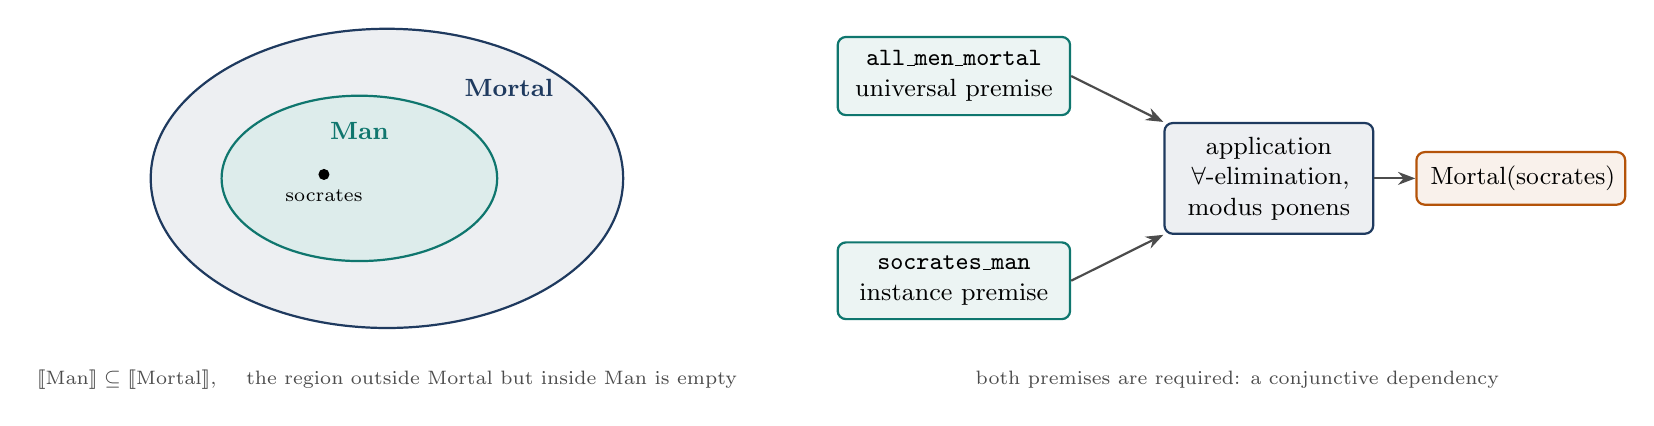
\begin{tikzpicture}[font=\small,>=Stealth]
\draw[thick,navy,fill=navy!8] (0,0) ellipse (3.0 and 1.9);
\draw[thick,teal,fill=teal!14] (-0.35,0) ellipse (1.75 and 1.05);
\fill (-0.8,0.05) circle (2pt) node[below=2pt,font=\scriptsize]{socrates};
\node[teal,font=\small\bfseries] at (-0.35,0.6) {Man};
\node[navy,font=\small\bfseries] at (1.55,1.15) {Mortal};
\node[font=\scriptsize,text=black!70,align=center] at (0,-2.55) {$\llbracket\mathrm{Man}\rrbracket\subseteq\llbracket\mathrm{Mortal}\rrbracket$, \quad the region outside Mortal but inside Man is empty};
\node[box=teal,text width=2.6cm] (h1) at (7.2,1.3) {\texttt{all\_men\_mortal}\\ universal premise};
\node[box=teal,text width=2.6cm] (h2) at (7.2,-1.3) {\texttt{socrates\_man}\\ instance premise};
\node[box=navy,text width=2.3cm] (ap) at (11.2,0) {application\\ $\forall$-elimination, modus ponens};
\node[box=amber,text width=2.3cm] (co) at (14.4,0) {$\mathrm{Mortal}(\mathrm{socrates})$};
\draw[arr=black!70] (h1.east) -- (ap.north west);
\draw[arr=black!70] (h2.east) -- (ap.south west);
\draw[arr=black!70] (ap.east) -- (co.west);
\node[font=\scriptsize,text=black!70,align=center] at (10.8,-2.55) {both premises are required: a conjunctive dependency};
\end{tikzpicture}
}
\caption{The syllogism as class inclusion (left) and as a dependency graph (right). Containment represents the universal premise and the marked point represents the instance premise. The drawing establishes neither premise and specifies no lifetime.}
\label{fig:socrates}
\end{figure}



Nothing in this term resembles the Fibonacci proof, and the contrast is instructive. There is no induction, no generalization, and no transport, because the claim does not quantify over a process of unspecified length. The entire logical content is that a universally quantified statement may be specialized. The empirical content sits wholly in the two hypotheses, which the term takes as given. The inference is free only in the sense that deductive validity adds no further empirical premise. Producing, checking and storing the term are physical processes, and what those processes require is the subject of the later sections on the layers of correctness and the accounting of memory. Observing that Socrates survives to a given date contradicts nothing, because mortality fixes no terminal date, and no finite observation refutes the premise. The bare predicate supplies no survival-time distribution, so it makes no length of survival improbable; evidence of prolonged survival bears against the premise only through a mortality model of the kind introduced below, and the inference would remain valid throughout. This division between a certain inference and an uncertain premise recurs in the second half of the essay with the roles of the two parts made more interesting.

\subsection{A process-level reading of mortality}

The syllogism treats mortality as a primitive predicate. A more informative reading replaces it with a statement about a process, and here induction with a generalized starting state returns. Model the status of an organism as a Markov chain on a finite set of states, one of which is an absorbing terminal state at which the lifetime ends, and call the remaining states active. Viability is maintained away from equilibrium, so the premise that is physically meaningful is that from every active state there is a path to the terminal state of some bounded length $m$ that has probability at least $\varepsilon > 0$ of being taken, so that $\varepsilon$ is a lower bound on the block mortality probability. No numerical value of $\varepsilon$ is needed, only its positivity.

\begin{proposition}\label{prop:decay}
Under the premise above, for every starting state $s$ and every $j$, the survival probability ${}_{jm}p_{s} = \Pr_s(\tau > jm)$ is at most $(1-\varepsilon)^j$.
\end{proposition}

\begin{proof}
The statement is quantified over the starting state $s$, exactly as the Fibonacci lemma is quantified over $k$. For $j = 0$ the bound is $1$ and holds trivially. For the step, condition on the state reached after the first block of $m$ steps. With probability at most $1-\varepsilon$ that block avoids the terminal state, and from whichever active state it ends in, the induction hypothesis, available because $s$ was universally quantified, bounds the remaining $j$ blocks by $(1-\varepsilon)^j$. Multiplying gives $(1-\varepsilon)^{j+1}$, and the exponent $jm + m = (j+1)m$ closes the case. The arithmetic here is trivial, but the decomposition of the time horizon into blocks of length $m$ is itself a modeling choice, imposed by stating the mortality premise per block, so the transport is model-dependent in the same sense as the passage from cycles to elapsed time below, though much milder.
\end{proof}

The proposition establishes almost-sure absorption, which is a different proposition from the deterministic predicate used in the syllogism, even though the difference has little practical consequence for a single organism. The same argument bounds the future lifetime: the proposition gives ${}_{jm}p_{s} \le (1-\varepsilon)^{j}$, and since the survival function ${}_{t}p_{s} = \Pr_s(\tau > t)$ is nonincreasing in $t$, the expectation of life satisfies
\[
\E_s[\tau] = \sum_{t \ge 0} {}_{t}p_{s} \le m \sum_{j \ge 0} {}_{jm}p_{s} \le m \sum_{j \ge 0} (1-\varepsilon)^{j} = \frac{m}{\varepsilon}.
\]
Here the first inequality groups the times $t$ into blocks $jm \le t < (j+1)m$ and bounds each term in a block by the term at the start of the block. Neither statement fixes a terminal date. For comparison, a constant force of mortality $\mu$ in continuous time gives ${}_{t}p = e^{-\mu t}$ and an expectation of life $1/\mu$, and the block premise yields a geometric bound of the same form without assuming a constant force. The deterministic syllogism is the idealization in which probability one is treated as certainty, and for a machine that is expected to run forever the distinction is the whole question.

\section{What a Perpetual Motion Machine Must Do}

Two kinds of device are customarily distinguished. A machine of the first kind creates energy and is excluded by conservation. A machine of the second kind is a device operating in a cycle that draws heat $Q$ from a single reservoir at temperature $T$ and delivers an equal amount of work, so that energy is conserved and the first law is respected. The first law alone cannot exclude the second kind: a cycle that takes in heat $Q$ from the reservoir and delivers work $Q$ returns the device to its initial state with $\oint dU = 0$, so conservation is silent about it, and the exclusion must come from the second law, which the argument below recovers as a statement about probabilities. Only the second kind needs a probabilistic argument, and it is the subject of the rest of the essay. The microscopic dynamics of the whole system, device plus reservoir, is assumed to be reversible, which is the situation in which the claim has real content. If the dynamics were allowed to be dissipative at the fundamental level, irreversibility would be assumed rather than derived.

\section{The Combinatorial Interpretation}\label{sec:comb}

Let $\Omega$ be a finite set of microstates of the composite system and let $\Phi : \Omega \to \Omega$ be one cycle of the dynamics. Reversibility means that $\Phi$ is a bijection, and Liouville's theorem in the finite setting is the statement that a bijection preserves the counting measure $\mu$. A macrostate is a subset of $\Omega$, and Boltzmann's relation \cite{boltzmann1877} identifies the entropy of a macrostate $A$ with $\kB \ln \mu(A)$.

\begin{lemma}\label{lem:count}
For macrostates $A$ and $B$, the number of microstates in $A$ that $\Phi$ carries into $B$ is at most $\min(\mu(A), \mu(B))$. Hence, for nonempty $A$ and the uniform measure on $A$, the probability of passing from $A$ to $B$ is at most $\min\{1, \mu(B)/\mu(A)\} = \min\{1, \exp\big((S_B - S_A)/\kB\big)\}$.
\end{lemma}

\begin{proof}
The set of microstates in $A$ that land in $B$ is mapped injectively into $B$ by $\Phi$, so its size is at most $\mu(B)$, and it is a subset of $A$, so its size is at most $\mu(A)$. Dividing by $\mu(A)$ gives the stated bound.
\end{proof}

Apply this to the engine. The composite system must contain three parts: the device, a work-storage system that receives the output, and the reservoir. The reservoir is idealized as held at fixed temperature $T$, so that giving up heat $Q$ lowers its entropy by $Q/T$; for a finite reservoir this expression is an approximation. The device is assumed to return to its initial macrostate, and the storage system is assumed to hold the work in a purely mechanical degree of freedom whose entropy does not change. Both are explicit assumptions, and correlations between the storage system and the other parts would alter the accounting. The return of the device and of the storage system to unchanged entropy is what makes the ratio attributable entirely to the reservoir; the lemma itself applies to arbitrary macrostates, and the reservoir alone enters here only because of these two assumptions. Under them the ratio of macrostate sizes is $\exp(-Q/(\kB T))$, and the lemma bounds the fraction of initial microstates that produce the behavior by that quantity. The argument contains no appeal to an arrow of time. It is a pigeonhole argument, and the arrow enters only through the choice of initial measure, uniform on the starting macrostate. The reverse process, in which work is consumed and heat is deposited in the reservoir, raises the reservoir's entropy, so the ratio exceeds one, the minimum in the lemma is one, and no restriction follows. Since $Q$ is macroscopic and $\kB$ is tiny, the bound for the engine is astronomically small, but it is not zero, and this is the first place where the result differs in kind from the syllogism: it is a bound on a fraction, not a refutation of an instance.

\section{The Stochastic Interpretation}

The counting argument treats a single cycle. The strength of the stochastic formulation is that it handles repeated operation, which is the only operation that could properly be called perpetual. Let the device be driven by a periodic protocol while in contact with a bath at inverse temperature $\beta = 1/(\kB T)$, with state space finite and dynamics satisfying microscopic reversibility. The Jarzynski equality \cite{jarzynski1997} and its Crooks refinement \cite{crooks1999} state that the work $W$ done on a system initially in canonical equilibrium satisfies
\[
\E\big[e^{-\beta W}\big] = e^{-\beta \Delta F},
\]
where $\Delta F$ is the change of equilibrium free energy between the end and start of the protocol. For a complete cycle $\Delta F = 0$. The identity is derived here from its microscopic hypothesis, so that its scope is visible. Let $\gamma$ range over trajectories of the cycle, let $\tilde\gamma$ be the time reversal of $\gamma$, and let $P_F$ and $P_R$ be the trajectory distributions of the forward protocol and of the reversed protocol, each started from canonical equilibrium. The hypothesis, taken from the cited fluctuation-theorem literature and satisfied for example by Markov jump dynamics obeying local detailed balance, is the Crooks relation
\[
\frac{P_F(\gamma)}{P_R(\tilde\gamma)} = e^{\beta (W(\gamma) - \Delta F)},
\]
with $\gamma \mapsto \tilde\gamma$ a bijection between the supports.

\begin{lemma}\label{lem:jarzynski}
Under the Crooks relation, $\E_F[e^{-\beta (W - \Delta F)}] = 1$.
\end{lemma}

\begin{proof}
By the relation, $P_F(\gamma)\, e^{-\beta (W(\gamma) - \Delta F)} = P_R(\tilde\gamma)$ for every $\gamma$. Summing over $\gamma$ and using the bijection, $\E_F[e^{-\beta (W - \Delta F)}] = \sum_{\gamma} P_R(\tilde\gamma) = 1$, because $P_R$ is a probability distribution.
\end{proof}

A complete derivation of the relation for a finite, discrete-time, driven Markov model, with its hypotheses explicit, is given in Appendix~\ref{app:crooks}. The lemma is only as strong as its hypothesis. It does not assert that every physical protocol satisfies the Crooks relation, and the initial-equilibrium assumption matters.

\begin{proposition}\label{prop:jensen}
For one cycle from equilibrium, the mean work extracted is nonpositive, and the probability of extracting work at least $w$ is at most $e^{-\beta w}$.
\end{proposition}

\begin{proof}
Jensen's inequality gives $e^{-\beta \E[W]} \le \E[e^{-\beta W}] = 1$, so $\E[W] \ge 0$: on average the environment does work on the device rather than the reverse. For the tail, extracted work $w$ means $W \le -w$, so $e^{-\beta W} \ge e^{\beta w}$, and Markov's inequality applied to the nonnegative variable $e^{-\beta W}$ on the event $\{W \le -w\}$, with mean one, gives $\Pr(W \le -w) \le e^{-\beta w}$.
\end{proof}

The proposition is again about a single cycle, and a skeptic will reply that a machine need only win a little each cycle and run for long enough. Answering this requires a statement about the whole sequence of cycles, and here care is needed. The single-time identity $\E[e^{-\Sigma_t}] = 1$, where $\Sigma_t$ is the total stochastic entropy production up to time $t$, does not by itself make $e^{-\Sigma_t}$ a martingale, since constant expectation is much weaker than the conditional property. The martingale property of $e^{-\Sigma_t}$ is developed for stationary processes under specified assumptions in \cite{neri2017}, and those assumptions should be taken from that source and not from this summary; a self-contained derivation for a finite stationary chain is given in Appendix~\ref{app:stationary}. Moreover, the time-reversed trajectory of a periodically driven process on a window of length $t$ depends on $t$ through the reversed protocol, so the property cannot simply be assumed for a driven engine. The result is therefore stated as a conditional theorem with its hypotheses made explicit.

\medskip
\noindent\textbf{Hypothesis H1.} At cycle boundaries, $Z_n = e^{-\Sigma_n}$ is a nonnegative supermartingale with $Z_0 = 1$. This is the one-step statement, quantified over every state the process might occupy, which plays the role that $k$ plays in the Fibonacci lemma, and induction on the number of cycles carries it to all $n$. It holds with equality in the stationary setting of \cite{neri2017}, and for a given driven model it must be established independently.

\medskip
\noindent\textbf{Hypothesis H2.} The extracted work $E_n$ after $n$ cycles satisfies $\Sigma_n = -\beta E_n + \Gamma_n$ with $\Gamma_n \le \kappa$ for a constant $\kappa$ independent of $n$. Writing $U_n$ for the system energy and $p_n$ for the distribution at the $n$-th cycle boundary, and taking extracted work as positive, the standard single-bath accounting gives $\Gamma_n = -\ln p_n(X_n) + \ln p_0(X_0) - \beta (U_n - U_0)$, the change in stochastic system entropy together with the energy change. It is bounded when the energies are bounded and the state probabilities at cycle boundaries stay uniformly away from zero, which is a property of the model to be verified and does not follow from finiteness of the state space alone. Periodic driving does not by itself make an arbitrary initial distribution periodic. If the process is initialized in an invariant distribution of the one-cycle transition kernel, which is unique and has full support when that kernel is irreducible on a finite state space, then the boundary distribution is the same at every cycle boundary and uniform positivity holds. Convergence from other initial distributions requires further assumptions.

\begin{lemma}[Ville's maximal inequality]\label{lem:ville}
If $(Z_n)_{n \ge 0}$ is a nonnegative supermartingale with $Z_0 = 1$, then $\Pr(\exists\, n : Z_n \ge \lambda) \le \min\{1, 1/\lambda\}$ for every $\lambda > 0$.
\end{lemma}

The proof is by optional stopping and is given, together with the version for the supremum, in Appendix~\ref{app:martingale}.

\begin{proposition}\label{prop:ville}
Under H1 and H2,
\[
\Pr\big(\exists\, n : E_n \ge w\big) \le \min\{1,\, e^{\,\kappa - \beta w}\} .
\]
\end{proposition}

\begin{proof}
If $E_n \ge w$ then H2 gives $\Sigma_n \le -\beta w + \kappa$, equivalently $Z_n \ge e^{\beta w - \kappa}$. By Lemma~\ref{lem:ville}, a classical result proved in Appendix~\ref{app:martingale} and treated in a modern form in \cite{doob1953,howard2020}, a nonnegative supermartingale started at one reaches a level $\lambda > 0$ at any time with probability at most $\min\{1, 1/\lambda\}$. This supports the probabilistic step and does not establish H1 for any engine.
\end{proof}

\begin{corollary}[Expected best cumulative work]\label{cor:expmax}
Under H1 and H2, let $E^{*} = \sup_{n \ge 0} E_n$ with $E_0 = 0$. Then $\kappa \ge 0$ and
\[
\E[E^{*}] \le \frac{\kappa + 1}{\beta} = \kB T\,(\kappa + 1).
\]
\end{corollary}

\begin{proof}
Since $\Sigma_0 = 0$ and $E_0 = 0$, H2 gives $\Gamma_0 = 0 \le \kappa$. The variable $E^{*}$ is nonnegative, and $\{E^{*} > w\} \subseteq \{\exists\, n : E_n \ge w\}$, so by Proposition~\ref{prop:ville}
\[
\E[E^{*}] = \int_0^\infty \Pr(E^{*} > w)\,dw \le \int_0^\infty \min\{1, e^{\kappa - \beta w}\}\,dw = \frac{\kappa}{\beta} + \int_{\kappa/\beta}^\infty e^{\kappa - \beta w}\,dw = \frac{\kappa + 1}{\beta}.
\]
\end{proof}

The corollary bounds the expected best cumulative result over the whole trajectory, even if an observer retrospectively selects the most favorable stopping point. It is conditional on H1 and H2, and $E_n$ is net cumulative extracted work, so it is not a bound on gross work extracted before subtracting work invested.

The constant $\kappa$ is not in general an erasure cost, and the connection to Landauer accounting is taken up in the Bayesian and reversibility discussions below. The bound does not weaken as $n$ grows, so under the hypotheses no amount of running time converts an exponentially unlikely excursion into a likely one. Letting $w \to \infty$ gives $\Pr(\sup_n E_n = \infty) = 0$, because $\{\sup_n E_n = \infty\} \subseteq \{\exists n : E_n \ge w\}$ for every $w$ and the bound tends to $0$, so cumulative extracted work is bounded above almost surely, although the bound is random and there need not be a deterministic maximum. This excludes sustained positive asymptotic work extraction almost surely. The statement is indexed by cycle count; translating it into a statement about elapsed time requires a model of cycle duration, which is not supplied here.

\begin{figure}[tbp]
\centering
\resizebox{\textwidth}{!}{%
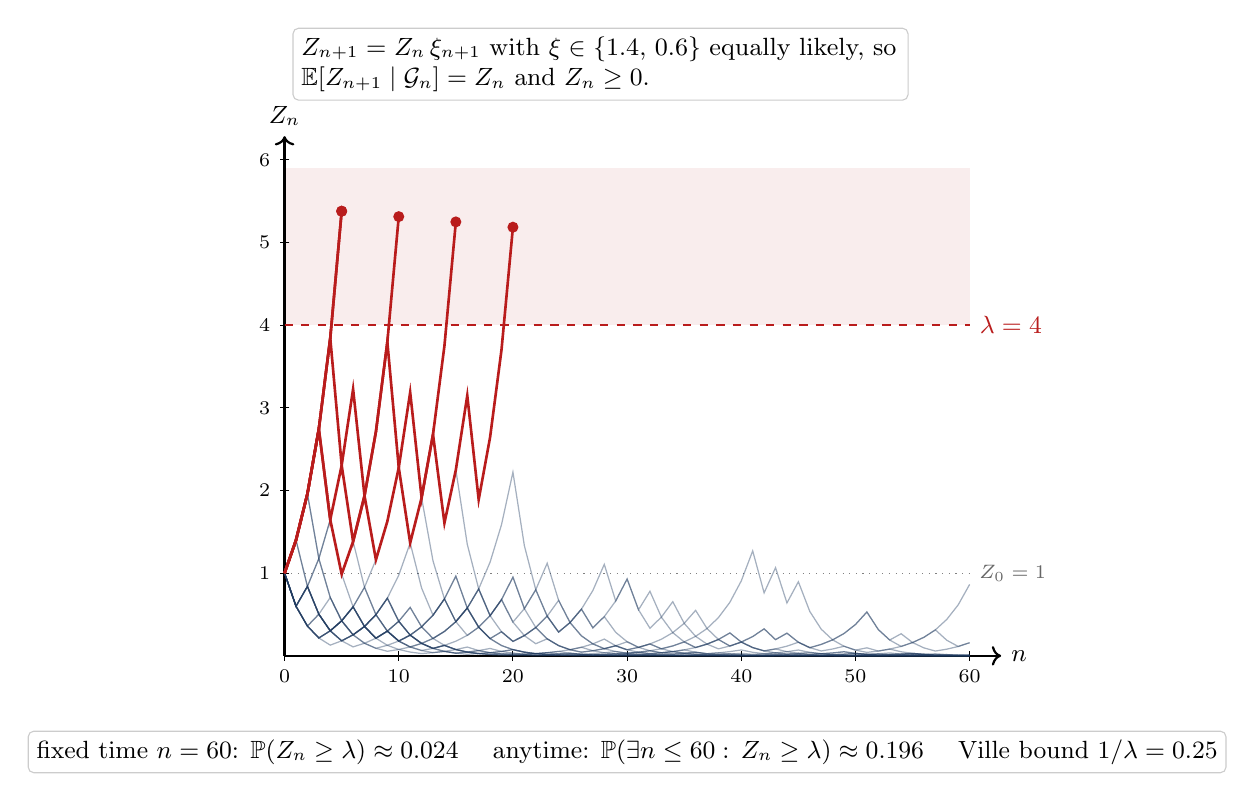
\begin{tikzpicture}[font=\small]
\fill[crimson!8] (0,4.200) rectangle (8.700,6.200);
\draw[->,thick] (0,0) -- (9.10,0) node[right]{$n$};
\draw[->,thick] (0,0) -- (0,6.60) node[above]{$Z_n$};
\draw (0.000,0.06)--(0.000,-0.06) node[below,font=\scriptsize]{0};
\draw (1.450,0.06)--(1.450,-0.06) node[below,font=\scriptsize]{10};
\draw (2.900,0.06)--(2.900,-0.06) node[below,font=\scriptsize]{20};
\draw (4.350,0.06)--(4.350,-0.06) node[below,font=\scriptsize]{30};
\draw (5.800,0.06)--(5.800,-0.06) node[below,font=\scriptsize]{40};
\draw (7.250,0.06)--(7.250,-0.06) node[below,font=\scriptsize]{50};
\draw (8.700,0.06)--(8.700,-0.06) node[below,font=\scriptsize]{60};
\draw (0.06,1.050)--(-0.06,1.050) node[left,font=\scriptsize]{1};
\draw (0.06,2.100)--(-0.06,2.100) node[left,font=\scriptsize]{2};
\draw (0.06,3.150)--(-0.06,3.150) node[left,font=\scriptsize]{3};
\draw (0.06,4.200)--(-0.06,4.200) node[left,font=\scriptsize]{4};
\draw (0.06,5.250)--(-0.06,5.250) node[left,font=\scriptsize]{5};
\draw (0.06,6.300)--(-0.06,6.300) node[left,font=\scriptsize]{6};
\draw[black!50,dotted] (0,1.050) -- (8.700,1.050) node[right,font=\scriptsize,black!60]{$Z_0=1$};
\draw[crimson,thick,dashed] (0,4.200) -- (8.700,4.200) node[right,crimson]{$\lambda=4$};
\draw[navy,line width=0.45pt,opacity=0.40] plot coordinates {(0.000,1.050) (0.145,0.630) (0.290,0.378) (0.435,0.227) (0.580,0.318) (0.725,0.191) (0.870,0.114) (1.015,0.160) (1.160,0.224) (1.305,0.314) (1.450,0.439) (1.595,0.263) (1.740,0.369) (1.885,0.516) (2.030,0.723) (2.175,0.434) (2.320,0.260) (2.465,0.364) (2.610,0.510) (2.755,0.714) (2.900,0.429) (3.045,0.600) (3.190,0.840) (3.335,0.504) (3.480,0.705) (3.625,0.423) (3.770,0.593) (3.915,0.356) (4.060,0.498) (4.205,0.299) (4.350,0.179) (4.495,0.108) (4.640,0.151) (4.785,0.090) (4.930,0.126) (5.075,0.177) (5.220,0.106) (5.365,0.149) (5.510,0.208) (5.655,0.125) (5.800,0.175) (5.945,0.245) (6.090,0.343) (6.235,0.206) (6.380,0.288) (6.525,0.173) (6.670,0.104) (6.815,0.145) (6.960,0.203) (7.105,0.122) (7.250,0.073) (7.395,0.102) (7.540,0.061) (7.685,0.086) (7.830,0.120) (7.975,0.169) (8.120,0.236) (8.265,0.330) (8.410,0.198) (8.555,0.119) (8.700,0.167)};
\draw[navy,line width=0.45pt,opacity=0.40] plot coordinates {(0.000,1.050) (0.145,0.630) (0.290,0.378) (0.435,0.529) (0.580,0.318) (0.725,0.445) (0.870,0.267) (1.015,0.160) (1.160,0.096) (1.305,0.134) (1.450,0.081) (1.595,0.048) (1.740,0.029) (1.885,0.041) (2.030,0.057) (2.175,0.034) (2.320,0.048) (2.465,0.029) (2.610,0.017) (2.755,0.024) (2.900,0.014) (3.045,0.009) (3.190,0.005) (3.335,0.007) (3.480,0.010) (3.625,0.006) (3.770,0.009) (3.915,0.012) (4.060,0.017) (4.205,0.024) (4.350,0.014) (4.495,0.020) (4.640,0.012) (4.785,0.007) (4.930,0.010) (5.075,0.014) (5.220,0.020) (5.365,0.012) (5.510,0.007) (5.655,0.004) (5.800,0.003) (5.945,0.004) (6.090,0.005) (6.235,0.007) (6.380,0.010) (6.525,0.014) (6.670,0.008) (6.815,0.005) (6.960,0.003) (7.105,0.004) (7.250,0.006) (7.395,0.008) (7.540,0.011) (7.685,0.016) (7.830,0.022) (7.975,0.013) (8.120,0.019) (8.265,0.026) (8.410,0.016) (8.555,0.009) (8.700,0.013)};
\draw[navy,line width=0.45pt,opacity=0.40] plot coordinates {(0.000,1.050) (0.145,0.630) (0.290,0.378) (0.435,0.529) (0.580,0.318) (0.725,0.445) (0.870,0.622) (1.015,0.373) (1.160,0.224) (1.305,0.314) (1.450,0.188) (1.595,0.263) (1.740,0.158) (1.885,0.095) (2.030,0.133) (2.175,0.080) (2.320,0.048) (2.465,0.029) (2.610,0.040) (2.755,0.056) (2.900,0.079) (3.045,0.047) (3.190,0.028) (3.335,0.017) (3.480,0.024) (3.625,0.033) (3.770,0.020) (3.915,0.028) (4.060,0.039) (4.205,0.024) (4.350,0.033) (4.495,0.046) (4.640,0.065) (4.785,0.039) (4.930,0.054) (5.075,0.033) (5.220,0.020) (5.365,0.012) (5.510,0.016) (5.655,0.023) (5.800,0.014) (5.945,0.008) (6.090,0.005) (6.235,0.007) (6.380,0.010) (6.525,0.014) (6.670,0.008) (6.815,0.011) (6.960,0.016) (7.105,0.022) (7.250,0.031) (7.395,0.019) (7.540,0.011) (7.685,0.007) (7.830,0.004) (7.975,0.002) (8.120,0.001) (8.265,0.001) (8.410,0.001) (8.555,0.001) (8.700,0.000)};
\draw[navy,line width=0.45pt,opacity=0.40] plot coordinates {(0.000,1.050) (0.145,0.630) (0.290,0.882) (0.435,0.529) (0.580,0.318) (0.725,0.445) (0.870,0.267) (1.015,0.373) (1.160,0.523) (1.305,0.732) (1.450,0.439) (1.595,0.263) (1.740,0.158) (1.885,0.095) (2.030,0.057) (2.175,0.034) (2.320,0.048) (2.465,0.067) (2.610,0.094) (2.755,0.056) (2.900,0.079) (3.045,0.047) (3.190,0.028) (3.335,0.040) (3.480,0.056) (3.625,0.033) (3.770,0.020) (3.915,0.012) (4.060,0.007) (4.205,0.004) (4.350,0.006) (4.495,0.008) (4.640,0.012) (4.785,0.007) (4.930,0.010) (5.075,0.006) (5.220,0.008) (5.365,0.005) (5.510,0.003) (5.655,0.004) (5.800,0.003) (5.945,0.002) (6.090,0.002) (6.235,0.003) (6.380,0.004) (6.525,0.002) (6.670,0.003) (6.815,0.005) (6.960,0.003) (7.105,0.002) (7.250,0.001) (7.395,0.001) (7.540,0.000) (7.685,0.001) (7.830,0.001) (7.975,0.000) (8.120,0.000) (8.265,0.000) (8.410,0.000) (8.555,0.000) (8.700,0.000)};
\draw[navy,line width=0.45pt,opacity=0.40] plot coordinates {(0.000,1.050) (0.145,0.630) (0.290,0.882) (0.435,0.529) (0.580,0.318) (0.725,0.445) (0.870,0.267) (1.015,0.373) (1.160,0.224) (1.305,0.134) (1.450,0.188) (1.595,0.113) (1.740,0.068) (1.885,0.095) (2.030,0.133) (2.175,0.186) (2.320,0.260) (2.465,0.364) (2.610,0.219) (2.755,0.131) (2.900,0.079) (3.045,0.047) (3.190,0.028) (3.335,0.017) (3.480,0.024) (3.625,0.014) (3.770,0.009) (3.915,0.005) (4.060,0.003) (4.205,0.002) (4.350,0.001) (4.495,0.001) (4.640,0.000) (4.785,0.000) (4.930,0.000) (5.075,0.000) (5.220,0.000) (5.365,0.000) (5.510,0.001) (5.655,0.000) (5.800,0.000) (5.945,0.001) (6.090,0.000) (6.235,0.000) (6.380,0.000) (6.525,0.000) (6.670,0.000) (6.815,0.000) (6.960,0.000) (7.105,0.000) (7.250,0.000) (7.395,0.000) (7.540,0.000) (7.685,0.000) (7.830,0.000) (7.975,0.000) (8.120,0.000) (8.265,0.000) (8.410,0.000) (8.555,0.000) (8.700,0.000)};
\draw[navy,line width=0.45pt,opacity=0.40] plot coordinates {(0.000,1.050) (0.145,0.630) (0.290,0.882) (0.435,1.235) (0.580,0.741) (0.725,0.445) (0.870,0.622) (1.015,0.373) (1.160,0.224) (1.305,0.314) (1.450,0.439) (1.595,0.615) (1.740,0.369) (1.885,0.516) (2.030,0.723) (2.175,1.012) (2.320,0.607) (2.465,0.364) (2.610,0.510) (2.755,0.714) (2.900,1.000) (3.045,0.600) (3.190,0.840) (3.335,1.176) (3.480,0.705) (3.625,0.423) (3.770,0.593) (3.915,0.356) (4.060,0.498) (4.205,0.697) (4.350,0.976) (4.495,0.585) (4.640,0.820) (4.785,0.492) (4.930,0.688) (5.075,0.413) (5.220,0.578) (5.365,0.347) (5.510,0.486) (5.655,0.680) (5.800,0.952) (5.945,1.333) (6.090,0.800) (6.235,1.120) (6.380,0.672) (6.525,0.941) (6.670,0.564) (6.815,0.339) (6.960,0.203) (7.105,0.284) (7.250,0.398) (7.395,0.557) (7.540,0.334) (7.685,0.201) (7.830,0.120) (7.975,0.169) (8.120,0.101) (8.265,0.061) (8.410,0.085) (8.555,0.119) (8.700,0.167)};
\draw[navy,line width=0.45pt,opacity=0.40] plot coordinates {(0.000,1.050) (0.145,1.470) (0.290,0.882) (0.435,0.529) (0.580,0.741) (0.725,0.445) (0.870,0.267) (1.015,0.373) (1.160,0.523) (1.305,0.732) (1.450,0.439) (1.595,0.263) (1.740,0.158) (1.885,0.221) (2.030,0.133) (2.175,0.080) (2.320,0.112) (2.465,0.067) (2.610,0.040) (2.755,0.056) (2.900,0.034) (3.045,0.020) (3.190,0.028) (3.335,0.017) (3.480,0.010) (3.625,0.006) (3.770,0.004) (3.915,0.005) (4.060,0.003) (4.205,0.004) (4.350,0.003) (4.495,0.002) (4.640,0.002) (4.785,0.001) (4.930,0.002) (5.075,0.001) (5.220,0.002) (5.365,0.001) (5.510,0.001) (5.655,0.002) (5.800,0.001) (5.945,0.001) (6.090,0.000) (6.235,0.000) (6.380,0.000) (6.525,0.000) (6.670,0.000) (6.815,0.000) (6.960,0.000) (7.105,0.000) (7.250,0.000) (7.395,0.000) (7.540,0.000) (7.685,0.001) (7.830,0.000) (7.975,0.000) (8.120,0.001) (8.265,0.001) (8.410,0.001) (8.555,0.002) (8.700,0.002)};
\draw[navy,line width=0.45pt,opacity=0.40] plot coordinates {(0.000,1.050) (0.145,0.630) (0.290,0.378) (0.435,0.227) (0.580,0.318) (0.725,0.445) (0.870,0.622) (1.015,0.871) (1.160,1.220) (1.305,1.708) (1.450,2.391) (1.595,1.434) (1.740,0.861) (1.885,0.516) (2.030,0.723) (2.175,0.434) (2.320,0.607) (2.465,0.364) (2.610,0.219) (2.755,0.131) (2.900,0.079) (3.045,0.047) (3.190,0.028) (3.335,0.017) (3.480,0.010) (3.625,0.006) (3.770,0.009) (3.915,0.012) (4.060,0.007) (4.205,0.010) (4.350,0.014) (4.495,0.020) (4.640,0.028) (4.785,0.039) (4.930,0.023) (5.075,0.033) (5.220,0.046) (5.365,0.027) (5.510,0.038) (5.655,0.054) (5.800,0.075) (5.945,0.045) (6.090,0.027) (6.235,0.038) (6.380,0.053) (6.525,0.074) (6.670,0.044) (6.815,0.027) (6.960,0.016) (7.105,0.022) (7.250,0.031) (7.395,0.019) (7.540,0.011) (7.685,0.007) (7.830,0.009) (7.975,0.013) (8.120,0.008) (8.265,0.005) (8.410,0.003) (8.555,0.004) (8.700,0.006)};
\draw[navy,line width=0.45pt,opacity=0.40] plot coordinates {(0.000,1.050) (0.145,0.630) (0.290,0.378) (0.435,0.227) (0.580,0.318) (0.725,0.191) (0.870,0.267) (1.015,0.373) (1.160,0.224) (1.305,0.314) (1.450,0.188) (1.595,0.113) (1.740,0.068) (1.885,0.041) (2.030,0.057) (2.175,0.080) (2.320,0.048) (2.465,0.029) (2.610,0.017) (2.755,0.010) (2.900,0.006) (3.045,0.004) (3.190,0.002) (3.335,0.003) (3.480,0.004) (3.625,0.003) (3.770,0.002) (3.915,0.001) (4.060,0.001) (4.205,0.001) (4.350,0.001) (4.495,0.001) (4.640,0.000) (4.785,0.001) (4.930,0.001) (5.075,0.000) (5.220,0.000) (5.365,0.000) (5.510,0.000) (5.655,0.000) (5.800,0.000) (5.945,0.000) (6.090,0.000) (6.235,0.000) (6.380,0.000) (6.525,0.000) (6.670,0.000) (6.815,0.000) (6.960,0.000) (7.105,0.000) (7.250,0.000) (7.395,0.000) (7.540,0.000) (7.685,0.000) (7.830,0.000) (7.975,0.000) (8.120,0.000) (8.265,0.000) (8.410,0.000) (8.555,0.000) (8.700,0.000)};
\draw[navy,line width=0.45pt,opacity=0.40] plot coordinates {(0.000,1.050) (0.145,0.630) (0.290,0.882) (0.435,0.529) (0.580,0.318) (0.725,0.191) (0.870,0.267) (1.015,0.373) (1.160,0.224) (1.305,0.314) (1.450,0.188) (1.595,0.263) (1.740,0.369) (1.885,0.221) (2.030,0.310) (2.175,0.434) (2.320,0.607) (2.465,0.850) (2.610,0.510) (2.755,0.714) (2.900,0.429) (3.045,0.257) (3.190,0.360) (3.335,0.216) (3.480,0.130) (3.625,0.078) (3.770,0.109) (3.915,0.065) (4.060,0.039) (4.205,0.055) (4.350,0.033) (4.495,0.046) (4.640,0.028) (4.785,0.017) (4.930,0.023) (5.075,0.033) (5.220,0.046) (5.365,0.027) (5.510,0.016) (5.655,0.023) (5.800,0.032) (5.945,0.019) (6.090,0.027) (6.235,0.038) (6.380,0.023) (6.525,0.032) (6.670,0.019) (6.815,0.027) (6.960,0.016) (7.105,0.010) (7.250,0.006) (7.395,0.003) (7.540,0.002) (7.685,0.003) (7.830,0.002) (7.975,0.002) (8.120,0.001) (8.265,0.002) (8.410,0.001) (8.555,0.001) (8.700,0.001)};
\draw[navy,line width=0.45pt,opacity=0.40] plot coordinates {(0.000,1.050) (0.145,1.470) (0.290,2.058) (0.435,2.881) (0.580,4.034) (0.725,2.420) (0.870,1.452) (1.015,0.871) (1.160,0.523) (1.305,0.314) (1.450,0.439) (1.595,0.263) (1.740,0.158) (1.885,0.095) (2.030,0.133) (2.175,0.080) (2.320,0.048) (2.465,0.067) (2.610,0.040) (2.755,0.024) (2.900,0.034) (3.045,0.020) (3.190,0.028) (3.335,0.040) (3.480,0.024) (3.625,0.033) (3.770,0.020) (3.915,0.012) (4.060,0.017) (4.205,0.024) (4.350,0.014) (4.495,0.008) (4.640,0.012) (4.785,0.007) (4.930,0.004) (5.075,0.006) (5.220,0.004) (5.365,0.005) (5.510,0.003) (5.655,0.002) (5.800,0.003) (5.945,0.004) (6.090,0.002) (6.235,0.003) (6.380,0.004) (6.525,0.006) (6.670,0.008) (6.815,0.005) (6.960,0.007) (7.105,0.010) (7.250,0.013) (7.395,0.019) (7.540,0.026) (7.685,0.037) (7.830,0.022) (7.975,0.031) (8.120,0.019) (8.265,0.011) (8.410,0.007) (8.555,0.009) (8.700,0.006)};
\draw[navy,line width=0.45pt,opacity=0.40] plot coordinates {(0.000,1.050) (0.145,1.470) (0.290,2.058) (0.435,1.235) (0.580,1.729) (0.725,1.037) (0.870,1.452) (1.015,2.033) (1.160,2.846) (1.305,3.985) (1.450,2.391) (1.595,1.434) (1.740,2.008) (1.885,2.812) (2.030,1.687) (2.175,2.362) (2.320,1.417) (2.465,0.850) (2.610,1.190) (2.755,1.666) (2.900,2.333) (3.045,1.400) (3.190,0.840) (3.335,0.504) (3.480,0.302) (3.625,0.423) (3.770,0.254) (3.915,0.152) (4.060,0.091) (4.205,0.128) (4.350,0.077) (4.495,0.046) (4.640,0.028) (4.785,0.039) (4.930,0.054) (5.075,0.033) (5.220,0.020) (5.365,0.012) (5.510,0.016) (5.655,0.010) (5.800,0.006) (5.945,0.008) (6.090,0.012) (6.235,0.016) (6.380,0.010) (6.525,0.006) (6.670,0.003) (6.815,0.005) (6.960,0.003) (7.105,0.002) (7.250,0.002) (7.395,0.001) (7.540,0.002) (7.685,0.003) (7.830,0.004) (7.975,0.006) (8.120,0.008) (8.265,0.005) (8.410,0.003) (8.555,0.004) (8.700,0.002)};
\draw[navy,line width=0.45pt,opacity=0.40] plot coordinates {(0.000,1.050) (0.145,1.470) (0.290,0.882) (0.435,0.529) (0.580,0.318) (0.725,0.191) (0.870,0.267) (1.015,0.160) (1.160,0.096) (1.305,0.058) (1.450,0.081) (1.595,0.113) (1.740,0.158) (1.885,0.095) (2.030,0.057) (2.175,0.034) (2.320,0.020) (2.465,0.029) (2.610,0.040) (2.755,0.024) (2.900,0.014) (3.045,0.020) (3.190,0.028) (3.335,0.040) (3.480,0.056) (3.625,0.078) (3.770,0.109) (3.915,0.152) (4.060,0.091) (4.205,0.128) (4.350,0.077) (4.495,0.108) (4.640,0.151) (4.785,0.090) (4.930,0.054) (5.075,0.076) (5.220,0.106) (5.365,0.149) (5.510,0.208) (5.655,0.291) (5.800,0.175) (5.945,0.105) (6.090,0.063) (6.235,0.088) (6.380,0.053) (6.525,0.032) (6.670,0.044) (6.815,0.027) (6.960,0.037) (7.105,0.052) (7.250,0.031) (7.395,0.019) (7.540,0.026) (7.685,0.016) (7.830,0.022) (7.975,0.031) (8.120,0.019) (8.265,0.011) (8.410,0.007) (8.555,0.004) (8.700,0.002)};
\draw[navy,line width=0.45pt,opacity=0.40] plot coordinates {(0.000,1.050) (0.145,1.470) (0.290,2.058) (0.435,1.235) (0.580,0.741) (0.725,0.445) (0.870,0.622) (1.015,0.373) (1.160,0.224) (1.305,0.314) (1.450,0.188) (1.595,0.263) (1.740,0.369) (1.885,0.516) (2.030,0.723) (2.175,1.012) (2.320,0.607) (2.465,0.364) (2.610,0.219) (2.755,0.306) (2.900,0.184) (3.045,0.257) (3.190,0.154) (3.335,0.216) (3.480,0.130) (3.625,0.078) (3.770,0.047) (3.915,0.065) (4.060,0.091) (4.205,0.055) (4.350,0.033) (4.495,0.046) (4.640,0.065) (4.785,0.039) (4.930,0.054) (5.075,0.076) (5.220,0.046) (5.365,0.027) (5.510,0.038) (5.655,0.023) (5.800,0.014) (5.945,0.008) (6.090,0.012) (6.235,0.016) (6.380,0.010) (6.525,0.006) (6.670,0.008) (6.815,0.005) (6.960,0.007) (7.105,0.010) (7.250,0.006) (7.395,0.003) (7.540,0.005) (7.685,0.007) (7.830,0.009) (7.975,0.013) (8.120,0.008) (8.265,0.005) (8.410,0.003) (8.555,0.004) (8.700,0.006)};
\draw[navy,line width=0.45pt,opacity=0.40] plot coordinates {(0.000,1.050) (0.145,0.630) (0.290,0.378) (0.435,0.227) (0.580,0.136) (0.725,0.191) (0.870,0.267) (1.015,0.373) (1.160,0.523) (1.305,0.732) (1.450,0.439) (1.595,0.615) (1.740,0.369) (1.885,0.221) (2.030,0.310) (2.175,0.434) (2.320,0.607) (2.465,0.850) (2.610,0.510) (2.755,0.714) (2.900,1.000) (3.045,0.600) (3.190,0.360) (3.335,0.504) (3.480,0.302) (3.625,0.423) (3.770,0.593) (3.915,0.830) (4.060,1.162) (4.205,0.697) (4.350,0.976) (4.495,0.585) (4.640,0.351) (4.785,0.492) (4.930,0.295) (5.075,0.413) (5.220,0.248) (5.365,0.149) (5.510,0.208) (5.655,0.125) (5.800,0.175) (5.945,0.245) (6.090,0.343) (6.235,0.206) (6.380,0.288) (6.525,0.173) (6.670,0.104) (6.815,0.062) (6.960,0.087) (7.105,0.122) (7.250,0.073) (7.395,0.044) (7.540,0.061) (7.685,0.086) (7.830,0.052) (7.975,0.031) (8.120,0.019) (8.265,0.011) (8.410,0.007) (8.555,0.004) (8.700,0.006)};
\draw[navy,line width=0.45pt,opacity=0.40] plot coordinates {(0.000,1.050) (0.145,0.630) (0.290,0.882) (0.435,0.529) (0.580,0.318) (0.725,0.445) (0.870,0.622) (1.015,0.871) (1.160,0.523) (1.305,0.314) (1.450,0.188) (1.595,0.263) (1.740,0.158) (1.885,0.095) (2.030,0.133) (2.175,0.080) (2.320,0.048) (2.465,0.029) (2.610,0.017) (2.755,0.010) (2.900,0.014) (3.045,0.020) (3.190,0.012) (3.335,0.007) (3.480,0.010) (3.625,0.014) (3.770,0.020) (3.915,0.012) (4.060,0.017) (4.205,0.024) (4.350,0.033) (4.495,0.020) (4.640,0.012) (4.785,0.017) (4.930,0.010) (5.075,0.006) (5.220,0.004) (5.365,0.005) (5.510,0.003) (5.655,0.002) (5.800,0.003) (5.945,0.002) (6.090,0.002) (6.235,0.001) (6.380,0.001) (6.525,0.000) (6.670,0.001) (6.815,0.000) (6.960,0.001) (7.105,0.001) (7.250,0.000) (7.395,0.000) (7.540,0.000) (7.685,0.000) (7.830,0.000) (7.975,0.000) (8.120,0.000) (8.265,0.000) (8.410,0.000) (8.555,0.000) (8.700,0.000)};
\draw[navy,line width=0.45pt,opacity=0.40] plot coordinates {(0.000,1.050) (0.145,0.630) (0.290,0.378) (0.435,0.227) (0.580,0.318) (0.725,0.445) (0.870,0.622) (1.015,0.373) (1.160,0.523) (1.305,0.732) (1.450,1.025) (1.595,1.434) (1.740,2.008) (1.885,1.205) (2.030,0.723) (2.175,0.434) (2.320,0.607) (2.465,0.850) (2.610,0.510) (2.755,0.306) (2.900,0.184) (3.045,0.257) (3.190,0.360) (3.335,0.216) (3.480,0.130) (3.625,0.078) (3.770,0.047) (3.915,0.065) (4.060,0.091) (4.205,0.128) (4.350,0.077) (4.495,0.108) (4.640,0.065) (4.785,0.090) (4.930,0.126) (5.075,0.177) (5.220,0.106) (5.365,0.149) (5.510,0.089) (5.655,0.125) (5.800,0.175) (5.945,0.105) (6.090,0.063) (6.235,0.038) (6.380,0.023) (6.525,0.032) (6.670,0.019) (6.815,0.027) (6.960,0.037) (7.105,0.052) (7.250,0.031) (7.395,0.019) (7.540,0.011) (7.685,0.016) (7.830,0.022) (7.975,0.031) (8.120,0.019) (8.265,0.011) (8.410,0.016) (8.555,0.009) (8.700,0.006)};
\draw[navy,line width=0.45pt,opacity=0.40] plot coordinates {(0.000,1.050) (0.145,0.630) (0.290,0.882) (0.435,1.235) (0.580,1.729) (0.725,1.037) (0.870,0.622) (1.015,0.373) (1.160,0.523) (1.305,0.314) (1.450,0.188) (1.595,0.113) (1.740,0.158) (1.885,0.221) (2.030,0.310) (2.175,0.434) (2.320,0.607) (2.465,0.364) (2.610,0.219) (2.755,0.306) (2.900,0.184) (3.045,0.257) (3.190,0.360) (3.335,0.504) (3.480,0.302) (3.625,0.423) (3.770,0.254) (3.915,0.152) (4.060,0.213) (4.205,0.128) (4.350,0.179) (4.495,0.108) (4.640,0.151) (4.785,0.211) (4.930,0.295) (5.075,0.177) (5.220,0.248) (5.365,0.347) (5.510,0.208) (5.655,0.291) (5.800,0.175) (5.945,0.105) (6.090,0.063) (6.235,0.088) (6.380,0.123) (6.525,0.173) (6.670,0.104) (6.815,0.145) (6.960,0.203) (7.105,0.284) (7.250,0.398) (7.395,0.557) (7.540,0.334) (7.685,0.201) (7.830,0.281) (7.975,0.169) (8.120,0.236) (8.265,0.330) (8.410,0.463) (8.555,0.648) (8.700,0.907)};
\draw[crimson,line width=0.95pt] plot coordinates {(0.000,1.050) (0.145,1.470) (0.290,2.058) (0.435,2.881) (0.580,4.034) (0.725,5.647)};
\fill[crimson] (0.725,5.647) circle (2pt);
\draw[crimson,line width=0.95pt] plot coordinates {(0.000,1.050) (0.145,1.470) (0.290,2.058) (0.435,2.881) (0.580,4.034) (0.725,2.420) (0.870,3.388) (1.015,2.033) (1.160,2.846) (1.305,3.985) (1.450,5.578)};
\fill[crimson] (1.450,5.578) circle (2pt);
\draw[crimson,line width=0.95pt] plot coordinates {(0.000,1.050) (0.145,1.470) (0.290,2.058) (0.435,2.881) (0.580,1.729) (0.725,2.420) (0.870,1.452) (1.015,2.033) (1.160,1.220) (1.305,1.708) (1.450,2.391) (1.595,3.347) (1.740,2.008) (1.885,2.812) (2.030,3.936) (2.175,5.511)};
\fill[crimson] (2.175,5.511) circle (2pt);
\draw[crimson,line width=0.95pt] plot coordinates {(0.000,1.050) (0.145,1.470) (0.290,2.058) (0.435,2.881) (0.580,1.729) (0.725,1.037) (0.870,1.452) (1.015,2.033) (1.160,2.846) (1.305,3.985) (1.450,2.391) (1.595,1.434) (1.740,2.008) (1.885,2.812) (2.030,1.687) (2.175,2.362) (2.320,3.306) (2.465,1.984) (2.610,2.777) (2.755,3.888) (2.900,5.444)};
\fill[crimson] (2.900,5.444) circle (2pt);
\draw[crimson,line width=0.95pt] plot coordinates {(0.000,1.050) (0.145,1.470) (0.290,2.058) (0.435,2.881) (0.580,4.034) (0.725,5.647)};
\fill[crimson] (0.725,5.647) circle (2pt);
\node[panel2,anchor=south west,text width=7.6cm] at (0.1,7.05) {$Z_{n+1}=Z_n\,\xi_{n+1}$ with $\xi\in\{1.4,\,0.6\}$ equally likely, so $\mathbb E[Z_{n+1}\mid\mathcal G_n]=Z_n$ and $Z_n\ge 0$.};
\node[panel2,anchor=north,align=center] at (4.35,-0.95) {fixed time $n=60$: $\Pr(Z_n\ge\lambda)\approx0.024$ \quad anytime: $\Pr(\exists n\le 60:\,Z_n\ge\lambda)\approx0.196$ \quad Ville bound $1/\lambda=0.25$};
\end{tikzpicture}
}
\caption{Illustrative simulation of a nonnegative martingale (multiplier $1.4$ or $0.6$ with equal probability), not data from any engine. Five plotted paths, in red, are stopped at their first crossing of $\lambda = 4$. Over 40000 simulated paths of 60 steps, the fraction that cross $\lambda$ at some time is about 0.196 and the fraction above $\lambda$ at the fixed time $n = 60$ is about 0.024. Both lie below the Ville bound $1/\lambda = 0.25$, and the gap between them is the difference between a fixed-time and an anytime probability.}
\label{fig:ville}
\end{figure}


\begin{remark}
Two further assumptions are carried by the result. The protocol must not depend on the microstate, and the system must be re-equilibrated or have its initial distribution accounted for. The next section is about what happens when the first of these is dropped.
\end{remark}

\section{The Bayesian Interpretation}

A Bayesian reading begins from Jaynes's proposal \cite{jaynes1957} that the thermodynamic entropy of a macrostate is the Shannon entropy of the distribution over microstates that is maximally noncommittal given the macroscopic constraints. On this view the entropy does not belong to the microstate. It belongs to the state of knowledge of an agent who knows only the macrovariables. Liouville dynamics carries a distribution to another of equal entropy, so an agent who gathers no new data has uncertainty that stays fixed, while coarse-graining, the act of describing the later state with the same few macrovariables, is what makes the uncertainty appear to grow.

This reading names the only escape route from the preceding sections. A device that senses the microstate and conditions its protocol on what it senses can make the work distribution depart from the bound. The Szilard engine \cite{szilard1929} is the canonical case. The generalization of the Jarzynski equality to feedback control by Sagawa and Ueda \cite{sagawa2010} involves a trajectory-level information density
\[
i(x,y) = \ln \frac{p(y \mid x)}{p(y)},
\]
for microstate $x$ and measurement outcome $y$, whose expectation is the mutual information $I(X;Y)$, and yields two separate identities, which must not be combined:
\[
\E\big[e^{-\beta (W - \Delta F) - i}\big] = 1,
\qquad
\E\big[e^{-\beta (W - \Delta F)}\big] = \gamma ,
\]
where $W$ is the work done on the system, so that $W_{\mathrm{ext}} = -W$, and $\gamma$ is their efficacy parameter, which measures how effectively the feedback uses the information and is not constrained to be at most one. These identities are stated as used in this essay, and the precise definitions of $i$, $\gamma$ and the measurement model are those of the cited paper. Jensen's inequality, with the information-theoretic facts of Appendix~\ref{app:info}, turns each into an average-work bound, not a trajectory-by-trajectory allowance:
\[
\E[W_{\mathrm{ext}}] \le -\E[\Delta F] + \kB T\, I(X;Y),
\qquad
\E[W_{\mathrm{ext}}] \le -\E[\Delta F] + \kB T \ln \gamma .
\]
For the first bound, convexity of the exponential gives $\exp\big(-\beta\,\E[W - \Delta F] - \E[i]\big) \le \E\big[e^{-\beta (W - \Delta F) - i}\big] = 1$, and taking logarithms, $\beta\,\E[W_{\mathrm{ext}} + \Delta F] \le \E[i] = I(X;Y)$. The second bound is the same step applied to the identity whose right-hand side is $\gamma$. The first identity also bounds a joint event, $\Pr\big(\beta (W_{\mathrm{ext}} + \Delta F) - i \ge a\big) \le e^{-a}$, but a tail bound on the work alone requires further control of the information density $i$. Feedback therefore permits extraction of work on average up to roughly $\kB T$ times the information gained. The repair comes from treating the memory record as part of the machine. A cyclic controller with bounded memory must restore the relevant memory resources over its complete operating cycle, which need not occur after every elementary engine cycle and can proceed by uncomputation as well as by erasure. Two qualifications precede any bound. The correlations between the memory and the rest of the system must be tracked, since a reset that exploits correlated side information can cost less than one that does not, and the cost of restoring the memory to a standard state independent of the system must be included. The thermodynamic costs of measurement and erasure depend on the physical memory model and must be included in the accounting of the complete information-processing cycle \cite{sagawa2009}. For an idealized, energetically degenerate classical memory reset without exploiting correlated side information, Landauer's principle \cite{landauer1961}, together with Bennett's resolution of the demon paradox \cite{bennett1982}, assigns the erasure a minimum average heat transfer to the bath of $\kB T\, H(M)$, with the entropy $H(M)$ of the memory distribution measured in nats. In the quasistatic limit an ideal erasure transfers this heat while the total entropy production approaches zero, because the memory entropy decreases correspondingly, so heat transferred to the bath, dissipated work and total entropy production are different quantities. The mutual information between memory $M$ and system satisfies $I(X;M) \le H(M)$, since $I(X;M) = H(M) - H(M \mid X)$ and $H(M \mid X) \ge 0$ for a discrete memory, so in that setting the average heat transfer is at least $\kB T\, I(X;M)$. The two accounts need not coincide, since the memory entropy can exceed the information gained. Under the idealization that the remaining corrections vanish, the net extractable work over the full cycle is nonpositive on average and the closed-cycle bound is restored with the demon included. Landauer accounting prices specified logically irreversible operations. A necessary condition for performing $N$ successive such operations within an available energy budget is $\sum_{j=1}^{N} q_j^{\min} \le E_{\mathrm{available}}$, where $q_j^{\min}$ are applicable lower bounds on the energy that must be transferred to the bath. If the lower bounds exceed the budget, the operations are excluded under the model, and if they do not, feasibility remains unresolved. A uniform bound $q_j^{\min} \ge q_* > 0$ gives $N \le E_{\mathrm{available}}/q_*$, whereas merely positive costs can form a convergent series and bound nothing. The bounds are averages unless a pathwise statement is separately established, so an operation-count limit of this kind concerns average costs. This is the route toward the view of a running program as a metastable structure and not an immortal one \cite{flyxion2026}, and it does not by itself establish a universal finite lifetime for every program. In Bayesian language, a posterior update that lowers the agent's entropy is paid for at a physical exchange rate under the conditions above, and the books balance on average only when the agent is counted among the physical systems.

\begin{figure}[tbp]
\centering
\resizebox{\textwidth}{!}{%
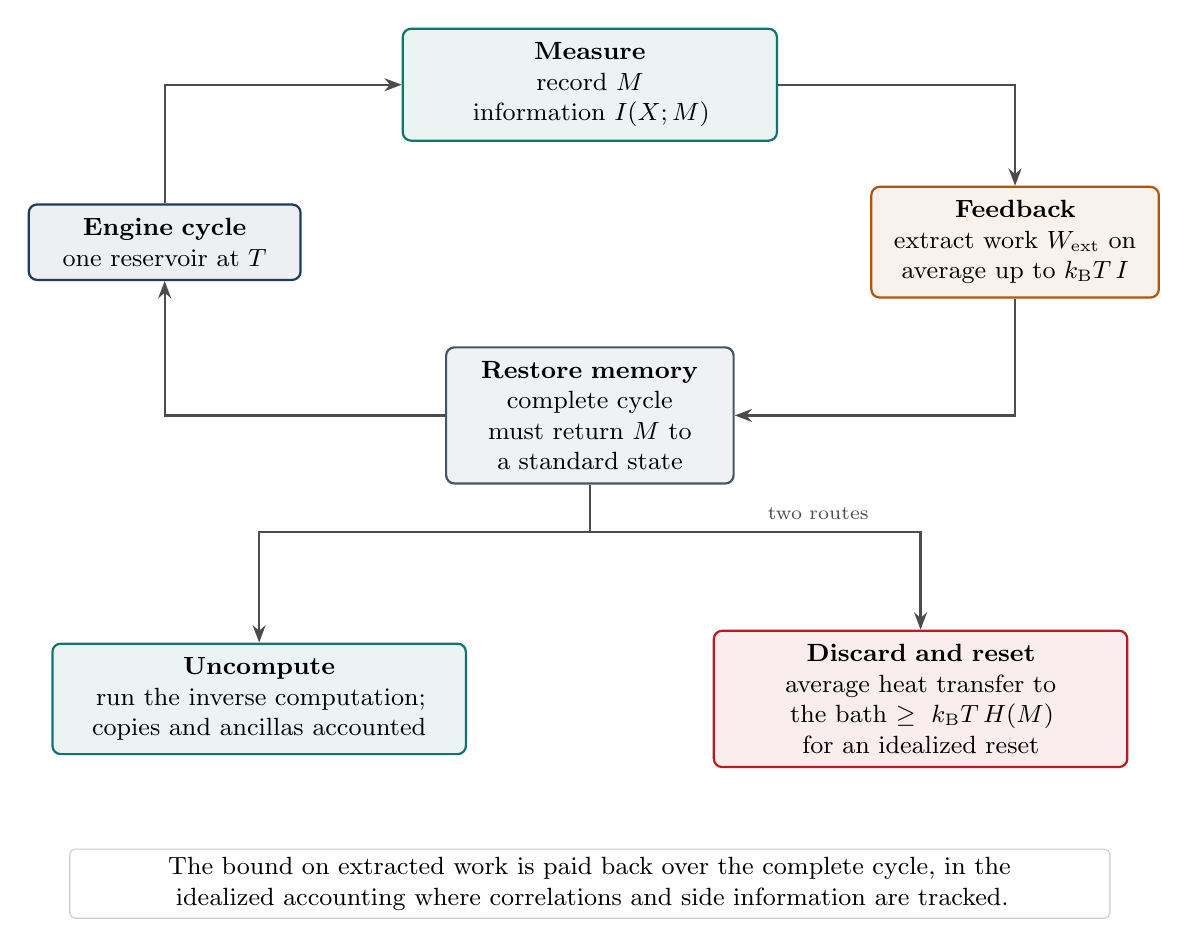
\begin{tikzpicture}[font=\small,>=Stealth]
\node[box=navy,text width=3.1cm] (E) at (0,0) {\textbf{Engine cycle}\\ one reservoir at $T$};
\node[box=teal,text width=4.4cm] (Me) at (5.4,2.0) {\textbf{Measure}\\ record $M$\\ information $I(X;M)$};
\node[box=amber,text width=3.3cm] (F) at (10.8,0) {\textbf{Feedback}\\ extract work $W_{\mathrm{ext}}$ on average up to $\kB T\,I$};
\node[box=slate,text width=3.3cm] (Re) at (5.4,-2.2) {\textbf{Restore memory}\\ complete cycle must return $M$ to a standard state};
\draw[arr=black!70] (E.north) |- (Me.west);
\draw[arr=black!70] (Me.east) -| (F.north);
\draw[arr=black!70] (F.south) |- (Re.east);
\draw[arr=black!70] (Re.west) -| (E.south);
\node[box=teal,text width=4.9cm] (U) at (1.2,-5.8) {\textbf{Uncompute}\\ run the inverse computation; copies and ancillas accounted};
\node[box=crimson,text width=4.9cm] (Er) at (9.6,-5.8) {\textbf{Discard and reset}\\ average heat transfer to the bath $\ge \kB T\,H(M)$ for an idealized reset};
\draw[arr=black!70] (Re.south) -- ++(0,-0.6) -| (U.north);
\draw[arr=black!70] (Re.south) -- ++(0,-0.6) -| (Er.north);
\node[font=\scriptsize,text=black!70,align=center] at (8.3,-3.45) {two routes};
\node[panel2,anchor=north,text width=13cm,align=center] at (5.4,-7.7) {The bound on extracted work is paid back over the complete cycle, in the idealized accounting where correlations and side information are tracked.};
\end{tikzpicture}
}
\caption{The complete cycle for a feedback engine with memory. Extraction by feedback is paid back over the full cycle. The memory is restored either by uncomputation, with the inverse computation and copies accounted, or by discarding and resetting, where an idealized, energetically degenerate classical reset without side information transfers at least $\kB T\,H(M)$ on average to the bath.}
\label{fig:cycle}
\end{figure}

\subsection{Why this is not a claim of certainty}

The Bayesian reading also clarifies what the impossibility claim is. Cromwell's rule counsels against assigning probability zero to hypotheses about the world, and that applies to the model as a whole. Within a model an event can have probability zero, as unbounded cumulative extraction does under H1 and H2, without being logically contradictory, and assigning it probability zero inside the model does not prevent revising the model. The thermodynamic theory assigns finite work-extracting fluctuations a bound that decays exponentially in the work and leaves positive credence on the hypotheses failing. A reported working machine of the second kind should therefore be weighed as evidence against one of the premises, namely the assumed reversibility of the underlying dynamics, the single-reservoir idealization, the absence of hidden feedback, or the integrity of the measurement, in proportion to how well each is independently supported. This is the same structure that governed the syllogism. The inference is a theorem, and the credence attaches to the hypotheses. A rational observer faced with an apparently indefinitely surviving Socrates and an apparently perpetual engine behaves similarly in both cases, by locating the error in the premises, though no finite observation of survival refutes mortality outright.

\section{The Dynamic Programming Interpretation}

A fourth reconstruction replaces the ensemble or the accounting identity by a recursion on a value function in the style of dynamic programming \cite{bellman1957}. The ingredients are a state space $S$, a set of admissible controls $A(s)$ at each state, a transition kernel, and a terminal or accumulated quantity to be evaluated. The recursion is obtained by conditioning on the first transition, and it corresponds to the generalized accumulator invariant in a precise way: the continuation value must be defined for every reachable state, so that after one transition the recursive argument applies again to the new state. The Fibonacci accumulator is the deterministic instance, with the carried pair of counts as state and no control. The quantification over $k$ in the Fibonacci lemma is the requirement that the value function be defined, and the recursion valid, at every state the process can reach.

\subsection{Survival}

Let $V \subseteq S$ be the active states and $P$ the transition matrix. Define the finite-horizon survival value by
\[
u_0(s) = \mathbf 1_V(s),
\qquad
u_{n+1}(s) = \mathbf 1_V(s) \sum_{s'} P(s,s')\, u_n(s').
\]
Then $u_n(s)$ is the probability of remaining in $V$ at times $0,\dots,n$ from $s$, that is, the $n$-step survival probability $u_n(s) = {}_{n}p_{s}$. Conditioning on the state after $a$ steps gives $u_{a+b}(s) = \E_s\big[\mathbf 1\{\text{active through } a\}\, u_b(S_a)\big]$. Suppose uniform block mortality holds, that is, $\Pr_s(\text{active through } m \text{ steps}) \le 1-\varepsilon$ for every active $s$. Then
\[
u_{jm}(s) \le (1-\varepsilon)^j \quad \text{for every } s .
\]
The proof is by induction on $j$ with $s$ universally quantified. The case $j=0$ is trivial, and
\[
u_{(j+1)m}(s) \le \Pr_s(\text{active through } m)\, \sup_{s'} u_{jm}(s') \le (1-\varepsilon)(1-\varepsilon)^j .
\]
If repair is treated as a control, the kernel becomes $P(s' \mid s, a)$ and the recursion takes a supremum over admissible actions, $u_{n+1}(s) = \mathbf 1_V(s) \sup_{a \in A(s)} \sum_{s'} P(s' \mid s, a)\, u_n(s')$. The same survival bound then requires a mortality condition uniform over admissible policies, not merely over states: for every policy, the probability of surviving $m$ steps from any active state must be at most $1-\varepsilon$. Repair by itself is compatible with the theorem, and it defeats the conclusion only if it defeats that uniform condition.

\subsection{Reachability of a work threshold}

Throughout this section the state space is finite, each action set $A(s)$ is finite and nonempty, and the work increment $r$ takes values in a finite set $R$, so that integrals are finite sums and suprema are maxima; the kernel notation extends to general spaces only under measurability and measurable-selection conditions that are not stated here. For the engine two optimization problems must be distinguished: maximizing expected cumulative work, and maximizing the probability of ever reaching a work threshold. The second is the relevant one for the bounds above. The state must include the system state, the protocol phase, and any memory or resource variables needed to make the transition law Markovian. Let a transition from state $s$ under action $a$ yield extracted work $r$ and next state $s'$ according to a kernel $K(ds', dr \mid s, a)$, and let $z$ denote the remaining work target. The finite-horizon reachability value satisfies
\[
v_0(s,z) = \mathbf 1_{\{z \le 0\}},
\qquad
v_{n+1}(s,z) =
\begin{cases}
1, & z \le 0,\\[1mm]
\displaystyle \sup_{a \in A(s)} \int v_n(s', z - r)\, K(ds', dr \mid s, a), & z > 0 .
\end{cases}
\]
The supremum represents feedback control. It cannot be introduced while retaining assumptions that were justified only for a fixed protocol, since any thermodynamic restriction used to bound the recursion must hold for every admissible action, with the controller's physical resources included in the state.

\subsection{The exponential bound as a supersolution}

Suppose a positive function $h$ satisfies, for every admissible state and action,
\[
\int e^{\beta r}\, h(s')\, K(ds', dr \mid s, a) \le h(s),
\qquad h(s) \ge h_{\min} > 0 .
\]

\begin{figure}[tbp]
\centering
\resizebox{\textwidth}{!}{%
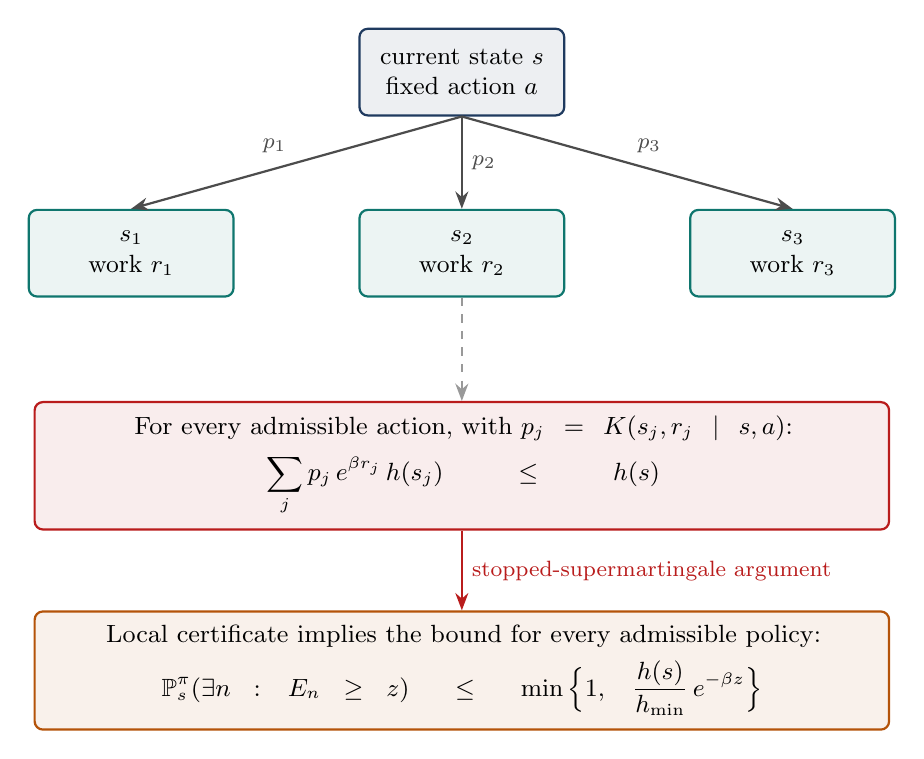
\begin{tikzpicture}[font=\small,>=Stealth]
\node[box=navy,minimum width=2.6cm,minimum height=1.1cm] (s) at (0,0) {current state $s$\\ fixed action $a$};
\node[box=teal,minimum width=2.6cm,minimum height=1.1cm] (s1) at (-4.2,-2.3) {$s_1$\\ work $r_1$};
\draw[arr=black!70] (s.south) -- node[above left,font=\footnotesize]{$p_1$} (s1.north);
\node[box=teal,minimum width=2.6cm,minimum height=1.1cm] (s2) at (0.0,-2.3) {$s_2$\\ work $r_2$};
\draw[arr=black!70] (s.south) -- node[right,font=\footnotesize]{$p_2$} (s2.north);
\node[box=teal,minimum width=2.6cm,minimum height=1.1cm] (s3) at (4.2,-2.3) {$s_3$\\ work $r_3$};
\draw[arr=black!70] (s.south) -- node[above right,font=\footnotesize]{$p_3$} (s3.north);
\node[box=crimson,text width=10.5cm] (c) at (0,-5.0) {For every admissible action, with $p_j=K(s_j,r_j\mid s,a)$:\\[4pt] $\displaystyle\sum_j p_j\,e^{\beta r_j}\,h(s_j)\;\le\;h(s)$};
\node[box=amber,text width=10.5cm] (r) at (0,-7.6) {Local certificate implies the bound for every admissible policy:\\[4pt] $\displaystyle\Pr^{\pi}_{s}(\exists n:\,E_n\ge z)\;\le\;\min\Big\{1,\;\frac{h(s)}{h_{\min}}\,e^{-\beta z}\Big\}$};
\draw[arr=crimson] (c.south) -- node[right,font=\footnotesize]{stopped-supermartingale argument} (r.north);
\draw[arr=black!40,dashed] (s2.south) -- (c.north);
\end{tikzpicture}
}
\caption{A local supersolution certificate for one action. Requiring the inequality for every admissible action makes the resulting reachability bound valid for every admissible policy. Three outcomes are shown schematically.}
\label{fig:certificate}
\end{figure}

\begin{proposition}\label{prop:bellman}
Under this supersolution condition, $v_n(s,z) \le \min\big\{1,\ (h(s)/h_{\min})\, e^{-\beta z}\big\}$ for all $n$, $s$ and $z$.
\end{proposition}

\begin{proof}
The induction is on $n$ with $s$ and $z$ universally quantified. For $z \le 0$ the value is $1$, and the right side equals $1$ because $h(s) \ge h_{\min}$ and $e^{-\beta z} \ge 1$; this covers $n = 0$ with $z > 0$ as well, where the value is $0$. For $z > 0$, the induction hypothesis at $(s', z - r)$ gives
\[
v_{n+1}(s,z) \le \sup_a \int \frac{h(s')}{h_{\min}}\, e^{-\beta (z-r)}\, K(ds', dr \mid s, a)
= \frac{e^{-\beta z}}{h_{\min}} \sup_a \int e^{\beta r}\, h(s')\, K(ds', dr \mid s, a)
\le \frac{h(s)}{h_{\min}}\, e^{-\beta z},
\]
and the bound by $1$ holds trivially.
\end{proof}

\begin{corollary}[Deterministic profitable cycle]\label{cor:cycle}
Suppose a supersolution $h$ exists, and that admissible actions $a_0, \dots, a_{m-1}$ produce, with probability one, transitions $s_0 \to s_1 \to \cdots \to s_m = s_0$ with extracted increments $r_0, \dots, r_{m-1}$. Then $\sum_{j=0}^{m-1} r_j \le 0$.
\end{corollary}

\begin{proof}
For a deterministic transition the supersolution inequality reads $e^{\beta r_j} h(s_{j+1}) \le h(s_j)$. Multiplying over $j$, and using $s_m = s_0$ so that the products $\prod_j h(s_{j+1})$ and $\prod_j h(s_j)$ coincide and are positive, gives $e^{\beta \sum_j r_j} \le 1$.
\end{proof}

A deterministic positive-work cycle is therefore a concrete obstruction to the existence of $h$. A single positive-work transition is compatible with the certificate, since it may consume potential, and returning to the starting state removes that explanation.

\begin{corollary}[Stationary mean work]\label{cor:stationary}
Under the supersolution condition, for every policy the potential-corrected work $Y_n = E_n + \beta^{-1}\big(\ln h(S_n) - \ln h(S_0)\big)$ satisfies $\E[Y_{n+1} - Y_n \mid \mathcal{G}_n] \le 0$. If a stationary policy induces a chain on $S$ with an invariant distribution $\mu$, then the mean work increment per step in that stationary regime satisfies $\E_\mu[r] \le 0$.
\end{corollary}

\begin{proof}
By Jensen's inequality for the concave logarithm, for every state $s$ and action $a$,
\[
\E\big[\beta r + \ln h(S') - \ln h(s) \mid s, a\big] \le \ln \E\!\left[\frac{e^{\beta r} h(S')}{h(s)} \,\Big|\, s, a\right] \le 0,
\]
by the supersolution inequality. This gives the first statement. In the stationary regime $S$ and $S'$ both have distribution $\mu$, so $\E_\mu[\ln h(S') - \ln h(S)] = 0$, and taking expectations in the displayed inequality leaves $\beta\,\E_\mu[r] \le 0$.
\end{proof}

The corollary gives an average-work consequence of the same certificate that yields the exponential crossing bound. Temporary extraction can be financed by a change of state, but stationary operation cannot continually spend a bounded state resource.

The proofs of this section are given in full for the finite model in Appendix~\ref{app:bellman}. The values $v_n$ are nondecreasing in $n$. Indeed $v_0 \le v_1$, because $v_0$ vanishes for $z > 0$ and both equal $1$ for $z \le 0$, and the recursion operator is monotone, since integrals and suprema preserve inequalities between integrands, so $v_n \le v_{n+1}$ implies $v_{n+1} \le v_{n+2}$. Let $\tau_z$ be the first time the cumulative extracted work reaches the target $z$. For each policy $\pi$, monotone convergence gives $\Pr^{\pi}(\tau_z < \infty) = \sup_n \Pr^{\pi}(\tau_z \le n)$. The optimized infinite-horizon reachability probability is $\sup_\pi \sup_n \Pr^{\pi}(\tau_z \le n) = \sup_n \sup_\pi \Pr^{\pi}(\tau_z \le n)$, and in a finite model the standard dynamic programming argument identifies each Bellman value $v_n$ with the finite-horizon policy supremum $\sup_\pi \Pr^{\pi}(\tau_z \le n)$. For finite state and action spaces the identification follows by induction on $n$: for $n = 0$ both sides equal $\mathbf 1_{\{z \le 0\}}$, and for the step, the supremum over policies that choose a first action and then follow any policy for the remaining $n$ steps is the supremum over first actions of the expectation of the $n$-horizon value, which is the recursion. Monotone convergence alone does not make this control-theoretic identification, and the bound passes to the limit through it. The corresponding nonnegative supermartingale is $e^{\beta E_n}\, h(S_n)/h(S_0)$, whose one-step supermartingale property is the supersolution inequality, and Ville's inequality applied to it reproduces the bound. The dynamic programming proof and the martingale proof are therefore two formulations of one certificate. H2 alone permits a boundary term $\Gamma_n$ that depends on time, the initial state or the history, so it does not by itself come from a state function. Under the additional assumption $\Gamma_n = \ln h(S_0) - \ln h(S_n)$ for a positive function $h$, one has $e^{-\Sigma_n} = e^{\beta E_n}\, h(S_n)/h(S_0)$, and the two certificates coincide, provided the supersolution inequality holds for the relevant initial states and admissible actions; a supermartingale property under one stationary law does not by itself establish an all-actions control certificate. In the stationary case with $p_n = p$ the boundary term has this form with $h(s) = p(s)\,e^{\beta U(s)}$. Without such a representation the Bellman certificate is a related sufficient condition and not a reformulation of an arbitrary pair H1 and H2.

The division of labor between the recursion and the supersolution is the point of this section. The Bellman recursion organizes the optimization problem and is the generalized accumulator invariant applied to a controlled process. The exponential supersolution contains the substantive thermodynamic assumption, namely that for every admissible action the exchange of work is constrained by a fixed potential $h$. Neither the recursion alone nor the existence of a value function supplies that assumption, and a controller with access to resources not included in $S$ may invalidate it.

\section{Church Numerals as Iteration}\label{sec:church}

In the untyped lambda calculus \cite{church1936,barendregt1984} a natural number is represented by the iteration it performs. The numeral for $n$ is
\[
\cn{n} = \lambda f.\,\lambda x.\; f^{n}(x), \qquad f^{0}(x) = x, \quad f^{k+1}(x) = f\big(f^{k}(x)\big),
\]
so that $\cn{0} = \lambda f.\lambda x.\,x$ and $\cn{3} = \lambda f.\lambda x.\, f(f(f\,x))$. The numeral stores no magnitude. It is a procedure that, given any function and any starting point, applies the function the stated number of times. This is the shape of the accumulator in the introduction, where the proof concerned the result of applying a one-step transition $n$ times from an arbitrary starting state, and the numeral $\cn{n}$ is a first-class name for the phrase ``apply $n$ times.''

Arithmetic then acts on iterators. Successor adds one application on the outside, addition sequences two iterators, multiplication nests them, and exponentiation applies one numeral to another:
\begin{align*}
\mathrm{succ} &= \lambda n.\lambda f.\lambda x.\; f\,(n\,f\,x), &
\mathrm{plus} &= \lambda m.\lambda n.\lambda f.\lambda x.\; m\,f\,(n\,f\,x), \\
\mathrm{mult} &= \lambda m.\lambda n.\lambda f.\; m\,(n\,f), &
\mathrm{exp} &= \lambda m.\lambda n.\; n\,m .
\end{align*}
For closed numerals the $\beta$-reductions give
\[
\mathrm{plus}\ \cn{m}\ \cn{n} =_{\beta} \cn{m+n},
\qquad
\mathrm{mult}\ \cn{m}\ \cn{n} =_{\beta\eta} \cn{mn},
\]
and $\mathrm{exp}\ \cn{m}\ \cn{n}$ applies the transformer $\cn{m}$ to $f$ a total of $n$ times, which yields $f^{m^{n}}$ and therefore $\cn{m^{n}}$ up to $\eta$-equivalence. The qualification is needed at $n = 0$: $\mathrm{exp}\ \cn{m}\ \cn{0} = \cn{0}\ \cn{m} \to_\beta \lambda x.\,x$, whereas $\cn{1} = \lambda f.\lambda x.\, f\,x$. These terms are $\eta$-equivalent and extensionally equal, but their $\beta$-normal forms differ, which makes the case a compact illustration of the distinction between conversion, syntax and extensional behavior drawn below. For addition, $\cn{n}\,f$ is the $n$-fold iterate of $f$ and $\cn{m}\,f\,(\cn{n}\,f\,x)$ applies the $m$-fold iterate after it. For multiplication, $\cn{m}$ applied to the $n$-fold iterate $\cn{n}\,f$ iterates that iterate $m$ times, which is $mn$ applications of $f$. In each case the operation transforms iterators and not magnitudes: addition composes two iterators in sequence, multiplication builds an iterator whose single step is itself an iteration, and exponentiation iterates that building step.

The reductions above rest on two facts about iteration of an ordinary function, which are not themselves lambda-calculus facts and are proved by induction.

\begin{lemma}\label{lem:iter}
For every function $f$ and all $m, n \in \mathbb{N}$, $f^{m}(f^{n}(x)) = f^{m+n}(x)$, and the $m$-fold iterate of $f^{n}$ equals $f^{mn}$.
\end{lemma}

\begin{proof}
For the first statement, induct on $m$: the case $m = 0$ is trivial, and $f^{m+1}(f^{n}(x)) = f\big(f^{m}(f^{n}(x))\big) = f\big(f^{m+n}(x)\big) = f^{m+n+1}(x)$. For the second, write $g = f^{n}$ and induct on $m$: $g^{m+1}(x) = f^{n}\big(g^{m}(x)\big) = f^{n}\big(f^{nm}(x)\big) = f^{n + nm}(x) = f^{n(m+1)}(x)$, using the first statement.
\end{proof}

Two senses of equality must be kept apart. Two terms $M$ and $N$ are extensionally equal when they act identically on every admissible argument, which for numerals means $M\,f\,x =_\beta N\,f\,x$ for every function $f$ and every starting point $x$. Equality of written expressions, meaning syntactic identity up to renaming of bound variables, is far finer. The expressions $\mathrm{plus}\ \cn{2}\ \cn{3}$ and $\cn{5}$ are written differently and are $\beta$-equal. A subtler case arises for $\mathrm{plus}\ m\ n$ and $\mathrm{plus}\ n\ m$ with $m$ and $n$ free variables. These reduce to the distinct $\beta$-normal forms $\lambda f.\lambda x.\; m\,f\,(n\,f\,x)$ and $\lambda f.\lambda x.\; n\,f\,(m\,f\,x)$, and no sequence of reductions identifies them. They are nonetheless extensionally equal on numerals, because every pair of closed numerals sends both to $\cn{m+n}$. The universal statement is a theorem about the explicitly defined Church numerals, the terms $\cn{k}$ for $k \in \mathbb{N}$, and not about arbitrary closed normal terms. It is established by the reduction $\cn{k}\,f\,x \to_\beta f^{k}(x)$, proved by induction on $k$, which sends both sides to $\cn{m+n}$, and it is not a rewriting derivation in the free variables.

The same distinction governs the Fibonacci equivalence proof. The branching program and the rolling-state program are structurally different expressions, and for a variable argument $n$ neither reduces to the other, so the proof assistant's conversion does not identify them. The theorem \texttt{fib\_eq} asserts a propositional equality $\forall n,\ \mathrm{fib2}\ n = \mathrm{fib}\ n$, which is an extensional equality of two programs for the same mathematical function. That is exactly why a generalized invariant is needed: the equality is a statement about all inputs and must be earned by induction, because it cannot be read off the text of either program. Church numerals give the rolling-state program a direct lambda-calculus form. With pairs encoded by $\mathrm{pair} = \lambda a.\lambda b.\lambda s.\; s\,a\,b$, projections $\mathrm{fst} = \lambda p.\; p\,(\lambda a.\lambda b.\,a)$ and $\mathrm{snd} = \lambda p.\; p\,(\lambda a.\lambda b.\,b)$, and the transition
\[
\Tm = \lambda p.\ \mathrm{pair}\ (\mathrm{snd}\ p)\ \big(\mathrm{plus}\ (\mathrm{fst}\ p)\ (\mathrm{snd}\ p)\big),
\qquad
\mathrm{fib} = \lambda n.\ \mathrm{fst}\ \big(n\ \Tm\ (\mathrm{pair}\ \cn{0}\ \cn{1})\big),
\]
the numeral $\cn{n}$ is the loop counter itself, and $\cn{n}\ \Tm\ p_0 =_\beta \Tm\big(\Tm(\cdots\Tm(p_0)\cdots)\big)$ with $n$ applications. A caution about size belongs here. Church numerals are unary, so a fully materialized numeral $\cn{F_n}$ has size $\Theta(F_n)$, which is exponential in $n$ even though the number of transition updates is linear. This output-size observation is all that is claimed, since the total cost of evaluation depends on the evaluation strategy, on sharing and on the cost model for substitution. The representation of the carried values nevertheless matters to resource counts, and it returns in the discussion of positional encodings below.

\section{Fibonacci Computation as Dynamic Programming with a Rolling State}\label{sec:fibdp}

The defining recurrence $F_{n+2} = F_{n+1} + F_n$ read as a program is a branching recursion. Counting every call, the number $C(n)$ of invocations satisfies $C(0) = C(1) = 1$ and $C(n+2) = C(n+1) + C(n) + 1$, and induction gives
\[
C(n) = 2F_{n+1} - 1 .
\]
Indeed the base cases hold, and $C(n+2) = (2F_{n+2} - 1) + (2F_{n+1} - 1) + 1 = 2F_{n+3} - 1$. Since $F_n$ grows like $\varphi^{n}/\sqrt{5}$ with $\varphi$ the golden ratio, the work is exponential. The cause is repeated evaluation of overlapping subproblems: the call tree for index $n$ contains the subproblem for every smaller index many times, while the subproblems themselves form a short chain, each index $k$ depending only on $k-1$ and $k-2$.

The state transition removes the repetition by carrying the two results that the next step needs. Define, on pairs of numbers,
\[
\Tm(a,b) = (b,\ a+b),
\]
where the sans-serif $\Tm$ denotes this map and not a temperature. If $\Tm$ is applied to a consecutive pair, the output is again a consecutive pair, so the pair is a sufficient summary of the past. The following invariant is the mathematical content of the accumulator lemma proved at the start of the essay. Closed forms, growth rates and Cassini's identity are collected in Appendix~\ref{app:fib}.

\begin{proposition}\label{prop:invariant}
For all $n, k \in \mathbb{N}$,
\[
\Tm^{n}(F_k, F_{k+1}) = (F_{n+k},\ F_{n+k+1}) .
\]
\end{proposition}

\begin{proof}
The induction is on $n$ with $k$ universally quantified. For $n = 0$ both sides equal $(F_k, F_{k+1})$. For the step, $\Tm^{n+1}(v) = \Tm^{n}(\Tm(v))$, and
\[
\Tm(F_k, F_{k+1}) = (F_{k+1},\ F_k + F_{k+1}) = (F_{k+1},\ F_{k+2}),
\]
which is the consecutive pair at index $k+1$. The induction hypothesis at $k+1$ gives
\[
\Tm^{n}(F_{k+1}, F_{k+2}) = (F_{n+(k+1)},\ F_{n+(k+1)+1}),
\]
and the index equality $n + (k+1) = (n+k) + 1$, which is the transport step of the Coq proof, converts this to $(F_{(n+1)+k}, F_{(n+1)+k+1})$. In Coq's notation the transport rewrites $n + S k$ to $S(n+k)$ by \texttt{Nat.add\_succ\_r}, while $(S\,n) + k$ reduces directly to $S(n+k)$, so both index expressions are propositionally equal to $S(n+k)$.
\end{proof}

Taking $k = 0$ and projecting gives $\mathrm{fst}\,\Tm^{n}(0,1) = F_n$, the correctness statement for the rolling-state program. The quantification over $k$ is not decoration. After one step the state is the pair at index $k+1$, and the hypothesis must apply to it, so the claim must hold for every starting pair of the form $(F_k, F_{k+1})$ and not merely for $(0,1)$. In the language of Section~\ref{sec:church} the invariant says that the iterator $\cn{n}\,\Tm$ sends every consecutive pair $n$ indices forward. The invariant has a matrix form, which is derived here. Write $\mathbf{J} = \begin{pmatrix}0&1\\1&1\end{pmatrix}$, a symmetric matrix, so that $\Tm$ is multiplication by $\mathbf{J}$ on pairs written as columns, and the row-vector convention gives the same map.

\begin{proposition}\label{prop:matrix}
For $n \ge 1$, $\ \mathbf{J}^{n} = \begin{pmatrix}F_{n-1}&F_n\\F_n&F_{n+1}\end{pmatrix}$. Consequently $F_{n+k} = F_{n-1}F_k + F_nF_{k+1}$ for $n \ge 1$ and all $k$, and $F_{2n} = F_n(2F_{n+1} - F_n)$ and $F_{2n+1} = F_n^{2} + F_{n+1}^{2}$.
\end{proposition}

\begin{proof}
The case $n = 1$ is $\mathbf{J} = \begin{pmatrix}F_0&F_1\\F_1&F_2\end{pmatrix}$. For the step,
\[
\mathbf{J}^{n+1} = \mathbf{J}^{n}\mathbf{J} = \begin{pmatrix}F_n&F_{n-1}+F_n\\F_{n+1}&F_n+F_{n+1}\end{pmatrix} = \begin{pmatrix}F_n&F_{n+1}\\F_{n+1}&F_{n+2}\end{pmatrix}
\]
By Proposition~\ref{prop:invariant}, $\mathbf{J}^{n}(F_k, F_{k+1})^{\top} = (F_{n+k}, F_{n+k+1})^{\top}$, and reading the first coordinate gives the addition formula. Setting $k = n$ gives $F_{2n} = F_{n-1}F_n + F_nF_{n+1} = F_n(F_{n+1} - F_n + F_{n+1})$, using $F_{n-1} = F_{n+1} - F_n$, and the second coordinate gives $F_{2n+1} = F_n^{2} + F_{n+1}^{2}$.
\end{proof}

This is dynamic programming with a rolling state \cite[Chapter~14]{cormen2022}. The subproblem table has one entry per index, and the dependence structure shows that only the two most recent entries are ever read, so the table may be replaced by a window of size two that is updated in place. Each subproblem is solved once, the number of transition steps for index $n$ is $n$, and the working storage is two values. In the terminology of the earlier Bellman section this is the uncontrolled deterministic case: the state is the pair, the kernel is the point mass at $\Tm(s)$, the accumulated quantity is the first coordinate, and the recursion $V_{n+1}(s) = V_n(\Tm(s))$ with $V_0 = \mathrm{fst}$ has the solution $V_n(s) = \mathrm{fst}\,\Tm^{n}(s)$. The continuation value is defined for every state $s$, not only for $(0,1)$, and that is the generalized invariant in dynamic programming dress.

\begin{figure}[tbp]
\centering
\resizebox{\textwidth}{!}{%
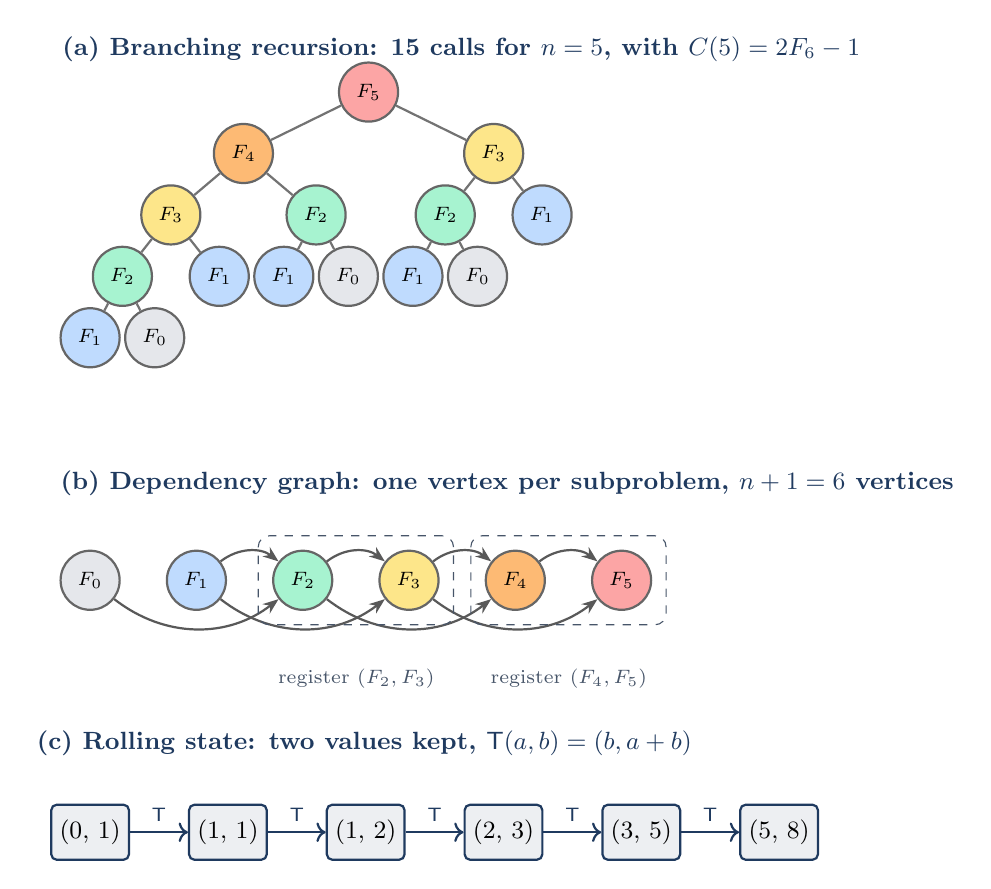
\begin{tikzpicture}[x=1cm,y=1cm,font=\small]
\begin{scope}[local bounding box=tree]
\node[treenode,fill=cF5] (t0) at (3.536,0.000) {$F_5$};
\node[treenode,fill=cF4] (t1) at (1.947,-0.780) {$F_4$};
\node[treenode,fill=cF3] (t2) at (1.025,-1.560) {$F_3$};
\node[treenode,fill=cF2] (t3) at (0.410,-2.340) {$F_2$};
\node[treenode,fill=cF1] (t4) at (0.000,-3.120) {$F_1$};
\node[treenode,fill=cF0] (t5) at (0.820,-3.120) {$F_0$};
\node[treenode,fill=cF1] (t6) at (1.640,-2.340) {$F_1$};
\node[treenode,fill=cF2] (t7) at (2.870,-1.560) {$F_2$};
\node[treenode,fill=cF1] (t8) at (2.460,-2.340) {$F_1$};
\node[treenode,fill=cF0] (t9) at (3.280,-2.340) {$F_0$};
\node[treenode,fill=cF3] (t10) at (5.125,-0.780) {$F_3$};
\node[treenode,fill=cF2] (t11) at (4.510,-1.560) {$F_2$};
\node[treenode,fill=cF1] (t12) at (4.100,-2.340) {$F_1$};
\node[treenode,fill=cF0] (t13) at (4.920,-2.340) {$F_0$};
\node[treenode,fill=cF1] (t14) at (5.740,-1.560) {$F_1$};
\draw[treeedge] (t3) -- (t4);
\draw[treeedge] (t3) -- (t5);
\draw[treeedge] (t2) -- (t3);
\draw[treeedge] (t2) -- (t6);
\draw[treeedge] (t7) -- (t8);
\draw[treeedge] (t7) -- (t9);
\draw[treeedge] (t1) -- (t2);
\draw[treeedge] (t1) -- (t7);
\draw[treeedge] (t11) -- (t12);
\draw[treeedge] (t11) -- (t13);
\draw[treeedge] (t10) -- (t11);
\draw[treeedge] (t10) -- (t14);
\draw[treeedge] (t0) -- (t1);
\draw[treeedge] (t0) -- (t10);
\end{scope}
\node[panel,anchor=north west] at ($(tree.north west)+(-0.1,0.45)$) {(a) Branching recursion: 15 calls for $n=5$, with $C(5)=2F_6-1$};
\begin{scope}[shift={(0,-6.20)}]
\node[treenode,fill=cF0] (d0) at (0.00,0) {$F_0$};
\node[treenode,fill=cF1] (d1) at (1.35,0) {$F_1$};
\node[treenode,fill=cF2] (d2) at (2.70,0) {$F_2$};
\node[treenode,fill=cF3] (d3) at (4.05,0) {$F_3$};
\node[treenode,fill=cF4] (d4) at (5.40,0) {$F_4$};
\node[treenode,fill=cF5] (d5) at (6.75,0) {$F_5$};
\draw[dagedge] (d1) to[bend left=38] (d2);
\draw[dagedge] (d0) to[bend right=38] (d2);
\draw[dagedge] (d2) to[bend left=38] (d3);
\draw[dagedge] (d1) to[bend right=38] (d3);
\draw[dagedge] (d3) to[bend left=38] (d4);
\draw[dagedge] (d2) to[bend right=38] (d4);
\draw[dagedge] (d4) to[bend left=38] (d5);
\draw[dagedge] (d3) to[bend right=38] (d5);
\node[draw=slate,dashed,rounded corners,fit=(d2)(d3),inner sep=5pt] {};
\node[draw=slate,dashed,rounded corners,fit=(d4)(d5),inner sep=5pt] {};
\node[font=\scriptsize,text=slate] at (3.38,-1.25) {register $(F_2,F_3)$};
\node[font=\scriptsize,text=slate] at (6.08,-1.25) {register $(F_4,F_5)$};
\node[panel,anchor=south west] at (-0.5,0.95) {(b) Dependency graph: one vertex per subproblem, $n+1=6$ vertices};
\end{scope}
\begin{scope}[shift={(0,-9.40)}]
\node[pair] (p0) at (0.00,0) {$(0,\,1)$};
\node[pair] (p1) at (1.75,0) {$(1,\,1)$};
\node[pair] (p2) at (3.50,0) {$(1,\,2)$};
\node[pair] (p3) at (5.25,0) {$(2,\,3)$};
\node[pair] (p4) at (7.00,0) {$(3,\,5)$};
\node[pair] (p5) at (8.75,0) {$(5,\,8)$};
\draw[->,rolling] (p0) -- node[above,font=\scriptsize]{$\mathsf T$} (p1);
\draw[->,rolling] (p1) -- node[above,font=\scriptsize]{$\mathsf T$} (p2);
\draw[->,rolling] (p2) -- node[above,font=\scriptsize]{$\mathsf T$} (p3);
\draw[->,rolling] (p3) -- node[above,font=\scriptsize]{$\mathsf T$} (p4);
\draw[->,rolling] (p4) -- node[above,font=\scriptsize]{$\mathsf T$} (p5);
\node[panel,anchor=south west] at (-0.8,0.85) {(c) Rolling state: two values kept, $\mathsf T(a,b)=(b,a+b)$};
\end{scope}
\end{tikzpicture}
}
\caption{Three views of the Fibonacci computation. (a) The call tree of the branching recursion for $n = 5$ has $C(5) = 2F_6 - 1 = 15$ nodes, with repeated subproblems in the same color. (b) The dependency graph has one vertex per subproblem, with arrows from an input value to the value that uses it, and dashed outlines mark the rolling register after two and after four updates. (c) The rolling implementation retains only the current consecutive pair.}
\label{fig:fibonacci}
\end{figure}

The count of arithmetic updates must be distinguished from the count of bit operations. The integer $F_n$ has approximately $n \log_2 \varphi \approx 0.694\,n$ bits. A schoolbook addition of two such numbers costs a number of bit operations proportional to their length, so the update at index $k$ costs $\Theta(k)$ bit operations, and the $n$ updates together cost $\Theta(n^2)$. The statement that the algorithm is linear counts additions as unit-cost operations, which is an idealization that fails once the integers outgrow a machine word. Asymptotically faster methods exist, for example the doubling identities of Proposition~\ref{prop:matrix} combined with fast multiplication, but they compute the same function and do not change what the rolling-state program is.

\section{Functional Completeness}\label{sec:fc}

A collection $\mathcal{F}$ of Boolean operations is functionally complete when every Boolean function $f : \{0,1\}^{n} \to \{0,1\}$ of positive arity $n \ge 1$ can be built from members of $\mathcal{F}$ by composition, with variables allowed to be reused, permuted and identified. In algebraic terms the clone generated by $\mathcal{F}$ contains every Boolean function of at least one variable \cite{wikifc}. The positive-arity restriction is deliberate, and its consequence is taken up below.

The negation of conjunction, written $A \nand B = \neg(A \land B)$, takes the value $0$ only when both arguments are $1$. It alone suffices, and the proof is constructive:
\begin{align*}
\neg A &= A \nand A, \\
A \land B &= (A \nand B) \nand (A \nand B), \\
A \lor B &= (A \nand A) \nand (B \nand B).
\end{align*}
Each identity is verified by cases. For the first, $A \nand A = \neg(A \land A) = \neg A$. For the second, $A \nand B = \neg(A \land B)$, and a double application of $\nand$ to the same argument negates it, so the result is $\neg\neg(A\land B) = A \land B$. For the third, $(A \nand A) \nand (B \nand B) = \neg(\neg A \land \neg B) = A \lor B$ by De Morgan's law. Since every Boolean function other than the constant zero is a disjunction of conjunctions of literals,
\[
f(x_1, \dots, x_n) = \bigvee_{v \,:\, f(v) = 1}\ \bigwedge_{i=1}^{n} x_i^{\,v_i},
\qquad x^{1} = x,\ x^{0} = \neg x,
\]
and the zero function is $x_1 \land \neg x_1$, the three identities translate any such expression into one using $\nand$ alone. The sufficiency of this single operation was published by Sheffer in 1913 \cite{sheffer1913}, and the standard reference article attributes unpublished earlier discovery to Peirce around 1880 \cite{wikifc}. The dual operation NOR is the only other binary operation with the property.

These identities establish expressive sufficiency and nothing more; normal forms and the classification of the binary Sheffer functions are proved in Appendix~\ref{app:bool}. They do not bound the size of the resulting expression, which for the disjunctive normal form above can reach order $2^{n}$ terms, and for any fixed finite complete basis of bounded arity, a counting argument due to Shannon \cite{shannon1949} shows that almost all Boolean functions of $n$ variables require circuits with at least on the order of $2^{n}/n$ gates, which is an $\Omega(2^{n}/n)$ lower bound, and counting alone does not give a matching asymptotic estimate. Circuit depth, memory requirements and physical energy consumption are likewise separate questions that the existence of an expression does not answer. Functional completeness must also be distinguished from two other notions that share the word. Completeness of a proof system concerns the relation between semantic validity and derivability, as in the theorem that every propositional tautology is provable, and it is a statement about proofs and not about which connectives are available. Computational universality concerns the ability to compute every computable function. Expressing every finite Boolean function does not by itself specify a machine of that kind, because a fixed circuit has fixed size, and universality additionally requires an account of unbounded memory and of iteration, such as a clocked register with a control loop and extensible storage, or the unrestricted abstraction and self-application of the lambda calculus.

\subsection{Post's Characterization}

Post's theorem \cite{post1941} gives a criterion that does not require building anything. Five classes of Boolean functions are relevant. A function $f$ of $n$ variables is monotone, written $f \in \mathcal{M}$, if $x \le y$ coordinatewise implies $f(x) \le f(y)$. It is affine, $f \in \mathcal{L}$, if $f(x) = \alpha_0 \oplus \alpha_1 x_1 \oplus \cdots \oplus \alpha_n x_n$ for constants $\alpha_i \in \{0,1\}$. It is self-dual, $f \in \mathcal{D}$, if $f(\neg x_1, \dots, \neg x_n) = \neg f(x_1, \dots, x_n)$. It is falsity-preserving, $f \in \mathcal{P}_0$, if $f(0,\dots,0) = 0$, and truth-preserving, $f \in \mathcal{P}_1$, if $f(1,\dots,1) = 1$. Each class contains the projections and is closed under composition, so a basis contained in one of them generates only functions in that class and cannot be complete. The necessity direction is checked directly. Let $h = f(g_1, \dots, g_r)$ with $f$ and all $g_i$ in the class. If they are monotone and $x \le y$, then $g_i(x) \le g_i(y)$ for each $i$, so $h(x) \le h(y)$. If they are affine, $h$ is a composition of affine maps over the two-element field and is affine. If they are self-dual, $h(\neg x) = f(\neg g(x)) = \neg f(g(x)) = \neg h(x)$. If they are falsity-preserving, $h(0) = f(g(0)) = f(0) = 0$, and the truth-preserving case is symmetric. This proves that a basis contained in one class is incomplete. The sufficiency direction, the converse below, is Post's theorem and is cited and not reproved here:
\[
\mathcal{F} \text{ is functionally complete} \iff \mathcal{F} \not\subseteq \mathcal{M},\ \ \mathcal{F} \not\subseteq \mathcal{L},\ \ \mathcal{F} \not\subseteq \mathcal{D},\ \ \mathcal{F} \not\subseteq \mathcal{P}_0,\ \ \mathcal{F} \not\subseteq \mathcal{P}_1 .
\]
The quantifier structure deserves emphasis. The condition is that for each class $\mathcal{C}$ there exists a member of $\mathcal{F}$ outside $\mathcal{C}$, and it is not that a single member lies outside all five classes. Different operations may supply different escapes. The basis $\{\land, \neg\}$ illustrates this. Negation lies outside $\mathcal{M}$, $\mathcal{P}_0$ and $\mathcal{P}_1$ but is both affine and self-dual, while conjunction lies outside $\mathcal{L}$ and $\mathcal{D}$ but is monotone and preserves both constants. Neither operation alone is complete, and together they escape every class.

For $\nand$ one operation supplies all five escapes. Its value at $(0,0)$ is $1$, so it is not falsity-preserving, and its value at $(1,1)$ is $0$, so it is not truth-preserving. It is not monotone because $(0,0) \le (1,1)$ while $\nand(0,0) = 1 > 0 = \nand(1,1)$. It is not self-dual because $\nand(0,1) = 1$ and $\nand(1,0) = 1$, whereas self-duality would force $\nand(1,0) = \neg\nand(0,1) = 0$. It is not affine because its polynomial over the two-element field is $A \nand B = 1 \oplus AB$, which contains the quadratic term $AB$. By Post's theorem $\{\nand\}$ is therefore complete, which agrees with the constructive derivation above.

The restriction to positive arity separates constant-valued functions from genuinely nullary constants. From $\nand$ one can derive, for a single variable $A$, the function $\mathbf{1}(A) = A \nand (A \nand A)$, since $A \nand A = \neg A$ and $A \nand \neg A = 1$ for both values of $A$, and then $\mathbf{0}(A) = \mathbf{1}(A) \nand \mathbf{1}(A)$. These are unary functions whose value happens not to depend on $A$. They do not provide a term with no inputs, because every $\nand$ gate consumes two input wires, so an expression built from $\nand$ alone always has at least one free variable. A circuit that needs an absolute constant, such as the initial pair $(0,1)$ of the Fibonacci register or the zero carry into the lowest bit position, must receive it as a supplied line or an initialized storage element, or must derive it from an input variable that is available, as $c_0 = \mathbf{0}(a_0)$ when an input bit $a_0$ exists. The criterion above is stated for bases of functions of positive arity, and it changes if nullary operations are admitted among the primitives, a variant not pursued here.

\section{NAND Realization of the Fibonacci Transition}\label{sec:nand}

The transition $\Tm(a,b) = (b, a+b)$ of Section~\ref{sec:fibdp} has three distinct descriptions that are easily conflated: the mathematical recurrence, which is a relation among integers; the algorithm, which iterates $\Tm$ on a carried pair; and the circuit, which realizes the addition in $\Tm$ with gates and holds the pair in storage. The correctness argument for the circuit composes local identities, and the local identity belongs to the full adder.

\subsection{The Full Adder and Its Local Invariant}

The exclusive or has the $\nand$ expression
\[
a \oplus b = (a \nand u) \nand (b \nand u), \qquad u = a \nand b,
\]
which is checked by computing $a \nand u = \neg(a \land \neg(a \land b)) = \neg a \lor b$ and, symmetrically, $b \nand u = a \lor \neg b$, whose $\nand$ is $\neg\big((\neg a \lor b) \land (a \lor \neg b)\big) = \neg(a \leftrightarrow b) = a \oplus b$. A full adder takes bits $a$, $b$ and a carry-in $c_{\mathrm{in}}$ and produces a sum bit $s$ and a carry-out $c_{\mathrm{out}}$. With $p = a \oplus b$,
\[
s = p \oplus c_{\mathrm{in}}, \qquad c_{\mathrm{out}} = (a \land b) \lor (p \land c_{\mathrm{in}}).
\]
In $\nand$ form, using the shared intermediates $u = a \nand b$ and $v = p \nand c_{\mathrm{in}}$,
\[
p = (a \nand u) \nand (b \nand u), \qquad
s = (p \nand v) \nand (c_{\mathrm{in}} \nand v), \qquad
c_{\mathrm{out}} = u \nand v,
\]
and the last equation holds because $u \nand v = \neg(\neg(ab) \land \neg(p c_{\mathrm{in}})) = ab \lor p c_{\mathrm{in}}$. The circuit uses nine $\nand$ gates, namely $u$, the three gates computing $p$ beyond $u$, $v$, the three gates computing $s$ beyond $v$, and $c_{\mathrm{out}}$, which is the standard count for a full adder built from $\nand$ alone. Its local arithmetic invariant, in which all five symbols are bits and the operations are ordinary addition and multiplication of integers, is
\[
a + b + c_{\mathrm{in}} = s + 2c_{\mathrm{out}} .
\]
To prove it, note first that for bits $x + y = (x \oplus y) + 2xy$, which is verified on the four input pairs. Then $a + b = p + 2ab$ and $p + c_{\mathrm{in}} = s + 2p c_{\mathrm{in}}$, so $a + b + c_{\mathrm{in}} = s + 2(ab + p c_{\mathrm{in}})$. The products $ab$ and $p c_{\mathrm{in}}$ cannot both equal $1$, because $ab = 1$ forces $a = b = 1$ and hence $p = 0$. Therefore $ab + p c_{\mathrm{in}} = ab \lor p c_{\mathrm{in}} = c_{\mathrm{out}}$, which gives the invariant. The invariant is a fact about a finite domain of eight input triples and could equally be verified by exhausting them.

\begin{figure}[tbp]
\centering
\resizebox{\textwidth}{!}{%
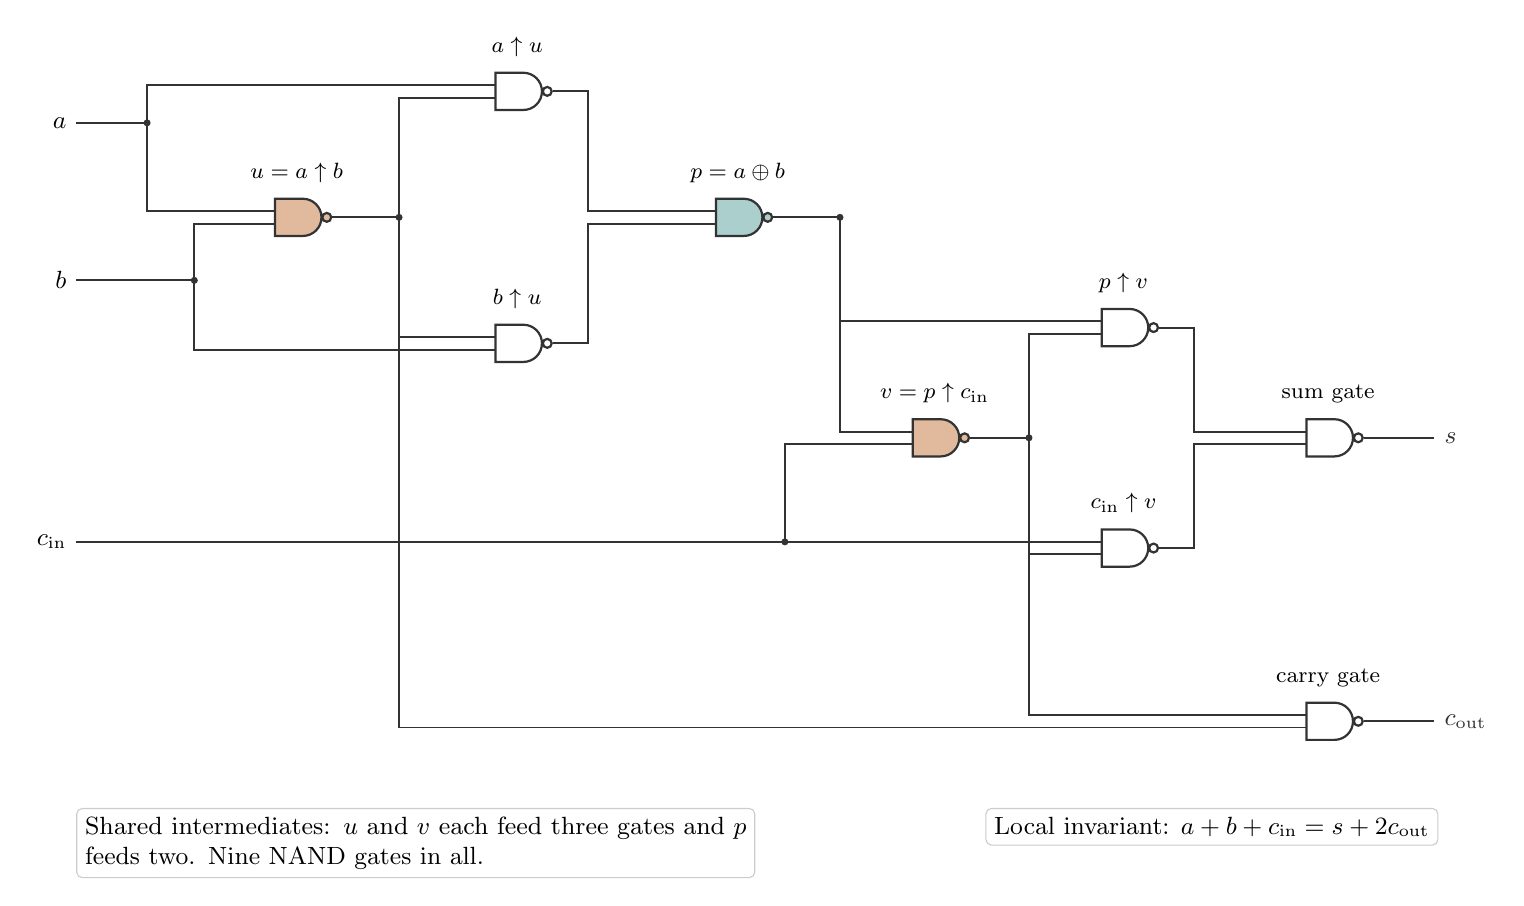
\begin{tikzpicture}[font=\small,>=Stealth]
\node[gate,fill=amber!40] (u) at (2.80,3.00) {};
\node[gate,fill=white] (t1) at (5.60,4.60) {};
\node[gate,fill=white] (t2) at (5.60,1.40) {};
\node[gate,fill=teal!35] (p) at (8.40,3.00) {};
\node[gate,fill=amber!40] (v) at (10.90,0.20) {};
\node[gate,fill=white] (t3) at (13.30,1.60) {};
\node[gate,fill=white] (t4) at (13.30,-1.20) {};
\node[gate,fill=white] (s) at (15.90,0.20) {};
\node[gate,fill=white] (co) at (15.90,-3.40) {};
\node[font=\footnotesize,above=2pt] at (u.north) {$u=a\uparrow b$};
\node[font=\footnotesize,above=2pt] at (t1.north) {$a\uparrow u$};
\node[font=\footnotesize,above=2pt] at (t2.north) {$b\uparrow u$};
\node[font=\footnotesize,above=2pt] at (p.north) {$p=a\oplus b$};
\node[font=\footnotesize,above=2pt] at (v.north) {$v=p\uparrow c_{\mathrm{in}}$};
\node[font=\footnotesize,above=2pt] at (t3.north) {$p\uparrow v$};
\node[font=\footnotesize,above=2pt] at (t4.north) {$c_{\mathrm{in}}\uparrow v$};
\node[font=\footnotesize,above=2pt] at (s.north) {sum gate};
\node[font=\footnotesize,above=2pt] at (co.north) {carry gate};
\node[left] (a) at (0,4.2) {$a$}; \node[left] (b) at (0,2.2) {$b$}; \node[left] (c) at (0,0 |- t4.input 1) {$c_{\mathrm{in}}$};
\coordinate (ja) at (0.9,4.2); \coordinate (jb) at (1.5,2.2); \coordinate (jc) at (9.0,0 |- t4.input 1);
\draw[wire] (0,4.2)--(ja); \draw[wire] (ja) |- (u.input 1); \draw[wire] (ja) |- (t1.input 1);
\draw[wire] (0,2.2)--(jb); \draw[wire] (jb) |- (u.input 2); \draw[wire] (jb) |- (t2.input 2);
\node[junc] at (ja) {}; \node[junc] at (jb) {};
\coordinate (ju) at (4.1,3.0); \draw[wire] (u.output)--(ju); \draw[wire] (ju) |- (t1.input 2); \draw[wire] (ju) |- (t2.input 1); \node[junc] at (ju) {};
\draw[wire] (ju) |- (co.input 2);
\draw[wire] (t1.output) -- ++(0.45,0) |- (p.input 1); \draw[wire] (t2.output) -- ++(0.45,0) |- (p.input 2);
\coordinate (jp) at (9.7,3.0); \draw[wire] (p.output)--(jp); \node[junc] at (jp) {}; \draw[wire] (jp) |- (v.input 1); \draw[wire] (jp) |- (t3.input 1);
\draw[wire] (c) -- (t4.input 1); \node[junc] at (jc) {}; \draw[wire] (jc) |- (v.input 2);
\coordinate (jv) at (12.1,0.2); \draw[wire] (v.output)--(jv); \node[junc] at (jv) {}; \draw[wire] (jv) |- (t3.input 2); \draw[wire] (jv) |- (t4.input 2); \draw[wire] (jv) |- (co.input 1);
\draw[wire] (t3.output) -- ++(0.45,0) |- (s.input 1); \draw[wire] (t4.output) -- ++(0.45,0) |- (s.input 2);
\draw[wire] (s.output) -- ++(0.9,0) node[right] {$s$}; \draw[wire] (co.output) -- ++(0.9,0) node[right] {$c_{\mathrm{out}}$};
\node[panel2,anchor=north west,text width=8.4cm] at (0.0,-4.5) {Shared intermediates: $u$ and $v$ each feed three gates and $p$ feeds two. Nine NAND gates in all.};
\node[panel2,anchor=north east] at (17.3,-4.5) {Local invariant: $a+b+c_{\mathrm{in}}=s+2c_{\mathrm{out}}$};
\end{tikzpicture}
}
\caption{A full adder built from nine NAND gates. Shaded gates are shared intermediates that feed several later gates, and wires cross without connection except at dots.}
\label{fig:adder}
\end{figure}

\subsection{Ripple-Carry Composition and Word Width}

Let $A = \sum_{i<L} a_i 2^{i}$ and $B = \sum_{i<L} b_i 2^{i}$ be $L$-bit numbers, set $c_0 = 0$, and define $(s_i, c_{i+1})$ as the output of a full adder on $(a_i, b_i, c_i)$. The carry is the carried state, and the correctness statement is generalized over its position in the same way as the Fibonacci lemma.

\begin{proposition}\label{prop:ripple}
For every $k \le L$,
\[
\sum_{i<k} (a_i + b_i)\,2^{i} = \sum_{i<k} s_i\,2^{i} + c_k\,2^{k} .
\]
Consequently $A + B = S + c_L\,2^{L}$, where $S = \sum_{i<L} s_i 2^{i}$.
\end{proposition}

\begin{proof}
For $k = 0$ both sides vanish because $c_0 = 0$. Assume the identity at $k$. Adding $(a_k + b_k)2^{k}$ to both sides gives, on the right, $\sum_{i<k} s_i 2^{i} + (c_k + a_k + b_k)2^{k}$. The local invariant states $c_k + a_k + b_k = s_k + 2c_{k+1}$, so the right side equals $\sum_{i\le k} s_i 2^{i} + c_{k+1}2^{k+1}$, which is the identity at $k+1$.
\end{proof}

\begin{figure}[tbp]
\centering
\resizebox{\textwidth}{!}{%
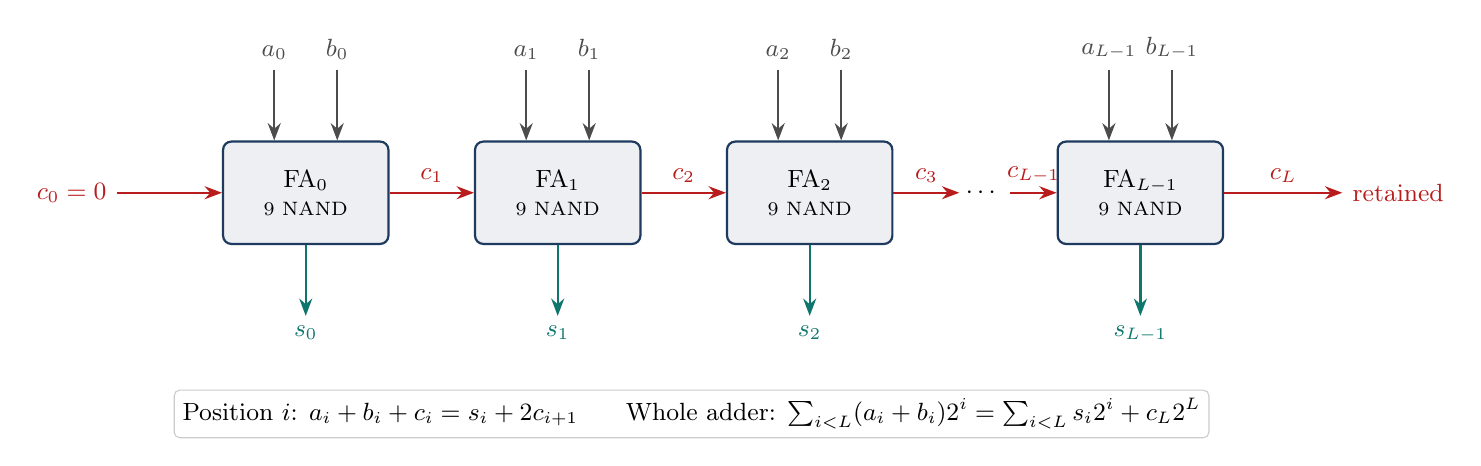
\begin{tikzpicture}[font=\small,>=Stealth]
\node[box=navy,minimum width=2.1cm,minimum height=1.3cm] (f0) at (0.00,0) {FA$_{0}$\\[-1pt]{\scriptsize 9 NAND}};
\draw[arr=black!70] ($(f0.north)+(-0.4,0.9)$) node[above]{$a_{0}$} -- ($(f0.north)+(-0.4,0)$);
\draw[arr=black!70] ($(f0.north)+(0.4,0.9)$) node[above]{$b_{0}$} -- ($(f0.north)+(0.4,0)$);
\draw[arr=teal] (f0.south) -- ++(0,-0.9) node[below]{$s_{0}$};
\node[box=navy,minimum width=2.1cm,minimum height=1.3cm] (f1) at (3.20,0) {FA$_{1}$\\[-1pt]{\scriptsize 9 NAND}};
\draw[arr=black!70] ($(f1.north)+(-0.4,0.9)$) node[above]{$a_{1}$} -- ($(f1.north)+(-0.4,0)$);
\draw[arr=black!70] ($(f1.north)+(0.4,0.9)$) node[above]{$b_{1}$} -- ($(f1.north)+(0.4,0)$);
\draw[arr=teal] (f1.south) -- ++(0,-0.9) node[below]{$s_{1}$};
\node[box=navy,minimum width=2.1cm,minimum height=1.3cm] (f2) at (6.40,0) {FA$_{2}$\\[-1pt]{\scriptsize 9 NAND}};
\draw[arr=black!70] ($(f2.north)+(-0.4,0.9)$) node[above]{$a_{2}$} -- ($(f2.north)+(-0.4,0)$);
\draw[arr=black!70] ($(f2.north)+(0.4,0.9)$) node[above]{$b_{2}$} -- ($(f2.north)+(0.4,0)$);
\draw[arr=teal] (f2.south) -- ++(0,-0.9) node[below]{$s_{2}$};
\node[box=navy,minimum width=2.1cm,minimum height=1.3cm] (f3) at (10.60,0) {FA$_{L{-}1}$\\[-1pt]{\scriptsize 9 NAND}};
\draw[arr=black!70] ($(f3.north)+(-0.4,0.9)$) node[above]{$a_{L{-}1}$} -- ($(f3.north)+(-0.4,0)$);
\draw[arr=black!70] ($(f3.north)+(0.4,0.9)$) node[above]{$b_{L{-}1}$} -- ($(f3.north)+(0.4,0)$);
\draw[arr=teal] (f3.south) -- ++(0,-0.9) node[below]{$s_{L{-}1}$};
\draw[arr=crimson] (-2.4,0) node[left]{$c_0=0$} -- (f0.west);
\draw[arr=crimson] (f0.east) -- node[above]{$c_1$} (f1.west);
\draw[arr=crimson] (f1.east) -- node[above]{$c_2$} (f2.west);
\draw[arr=crimson] (f2.east) -- node[above]{$c_3$} (8.3,0);
\node at (8.6,0) {$\cdots$};
\draw[arr=crimson] (8.95,0) -- node[above]{$c_{L-1}$} (f3.west);
\draw[arr=crimson] (f3.east) -- node[above]{$c_L$} ++(1.5,0) node[right]{retained};
\node[panel2,anchor=north] at (4.9,-2.5) {Position $i$: $a_i+b_i+c_i=s_i+2c_{i+1}$ \hspace{1.2em} Whole adder: $\sum_{i<L}(a_i+b_i)2^{i}=\sum_{i<L}s_i2^{i}+c_L2^{L}$};
\end{tikzpicture}
}
\caption{Ripple-carry composition of full adders. The carry is the carried state, and the identity at each position composes into the identity for the whole adder when the final carry $c_L$ is retained.}
\label{fig:ripple}
\end{figure}

The theorem is exact provided the final carry is retained, which yields an $(L+1)$-bit result, or is proved to vanish, which happens exactly when $A + B < 2^{L}$. A fixed-width circuit that discards $c_L$ computes addition modulo $2^{L}$, since then $S = (A+B) \bmod 2^{L}$. An arbitrary-precision implementation instead enlarges its storage as the values grow, so that the width is at least the length of the largest value. For the Fibonacci register this length grows linearly, as noted above, and an unbounded computation therefore requires a family of circuits indexed by width, or a machine with extensible memory.

The addition theorem supplies the arithmetic step in the accumulator invariant. Let $\mathrm{dec}_2$ denote the binary decoding of a bit-vector, and suppose a register holds bit-vectors $A_k, B_k$ with $\mathrm{dec}_2(A_k) = F_k$ and $\mathrm{dec}_2(B_k) = F_{k+1}$. One clock step sets $A' = B_k$ and $B' = $ the ripple-carry sum of $A_k$ and $B_k$. By Proposition~\ref{prop:ripple}, if $F_{k+2} < 2^{L}$, which holds at every step with $k+2 \le N+1$ when $F_{N+1} < 2^{L}$, then $\mathrm{dec}_2(B') = F_k + F_{k+1} = F_{k+2}$, so the register again holds a consecutive pair, now at index $k+1$. The register-level statement is therefore Proposition~\ref{prop:invariant} read through $\mathrm{dec}_2$, with the side condition that the width $L$ satisfies $F_{N+1} < 2^{L}$ for the largest index $N$ of interest.

\subsection{Recurrence, Algorithm, Circuit, and Finite Validation}

The three descriptions require three kinds of evidence. The recurrence is a specification and requires no proof of itself. The algorithm is correct for all $n$ by the induction of Proposition~\ref{prop:invariant}. The circuit is correct for all $n \le N$ by composing the full-adder invariant, Proposition~\ref{prop:ripple} and the register induction under the width condition. A reported check of the circuit's outputs against the reference values for every index from $0$ through $24$ is a finite computational validation of that composition. For a width of $17$ bits it exercises the sequence through $F_{25} = 75025 < 2^{17} = 131072$. The source and execution record of that experiment are not part of this essay, so it is described only by what a check of this form can establish. It establishes agreement on the twenty-five inputs tested and for the width used. It does not establish agreement for any other $n$, it does not by itself establish that the circuit is a correct adder on all inputs, and it says nothing about widths other than the one tested. The universal claim comes from the proofs, and the experiment can serve as a test of the implementation against them, in the way a finite sample tests a program whose correctness is argued separately.

\subsection{Sharing and Retained Intermediate Results}

The expression
\[
(A \nand B) \nand (A \nand B)
\]
and the circuit description
\[
x := A \nand B, \qquad A \land B := x \nand x
\]
compute the same Boolean function of $A$ and $B$. The second names the subcomputation $x$ and reuses its value, so only two gates are needed, while the first, read as a tree, contains the subexpression $A \nand B$ twice and counts three. A formula is naturally a tree, in which each occurrence of a subformula is a separate node, whereas a circuit is a directed acyclic graph in which one computed wire may feed several gates. The difference is not cosmetic. If $x_{k+1} = x_k \nand x_k$, then the circuit with one gate per stage has $k$ gates after $k$ stages, but the fully expanded tree has $G(k)$ gates with $G(k+1) = 2G(k) + 1$ and $G(0) = 0$, that is $G(k) = 2^{k} - 1$. The function itself is much simpler than either description: since $x \nand x = \neg x$, one has $x_k = x_0$ for even $k$ and $x_k = \neg x_0$ for odd $k$, so the minimum circuit size of the function is zero gates for even $k$, a bare wire, and one gate for odd $k$. The example therefore separates three quantities, the size of an expression, the size of its shared implementation, and the minimum circuit size of the function, and shows that sharing and algebraic simplification are distinct sources of economy. The full adder above uses sharing in the same way: the gate $u$ feeds both $p$ and $c_{\mathrm{out}}$, and $v$ feeds both $s$ and $c_{\mathrm{out}}$.

This is the same distinction as between the branching Fibonacci recursion and the memoized one. The call tree of the recursion unfolds a directed acyclic graph of subproblems with $n+1$ nodes, and the size of the call tree is the quantity $C(n) = 2F_{n+1} - 1$ computed above, which blows up for the same reason that the expanded formula does: shared nodes are recomputed at every occurrence. Sharing within a combinational circuit and storing values between Fibonacci iterations are related techniques for avoiding repeated work, but they require different mechanisms. Fan-out is sharing in space, and iteration is sharing in time, which requires a clock and a register. Sharing in a combinational circuit is fan-out, a wire carrying one value to several gates within a single evaluation and requiring no memory element. Storing the pair between iterations requires state: a register that holds the output of one step so that it is available as the input of the next, together with a clock to separate the steps. An $n$-step computation can be unrolled into a combinational directed acyclic graph containing $n$ adders, with wires carrying values forward, or it can be run on a single adder reused over $n$ clock cycles. The two designs implement one dependence graph, trading space for time.

\subsection{Boolean Expressiveness and Physical Reversibility}

The gate $\nand$ is logically irreversible: the three input pairs $(0,0)$, $(0,1)$ and $(1,0)$ all map to the output $1$, so the output does not determine the input. Functional completeness nevertheless establishes no universal energy cost per gate. It is a statement about which functions can be written, and it holds equally for sets of reversible gates used with auxiliary bits, so it cannot fix a thermodynamic price.

An irreversible Boolean function can be embedded in an injective computation by retaining information. For any $f : \{0,1\}^{n} \to \{0,1\}^{m}$ the map
\[
f^{\sharp}(x, y) = (x,\ y \oplus f(x))
\]
on $\{0,1\}^{n+m}$ is a bijection, since applying it twice returns the input, because $y \oplus f(x) \oplus f(x) = y$, and it computes $f(x)$ when the auxiliary register starts at $y = 0$. For $\nand$ this is the Toffoli gate $(a, b, y) \mapsto (a, b, y \oplus ab)$ with the auxiliary bit preset to $1$, because then the third output is $1 \oplus ab = a \nand b$, and the inputs $a$ and $b$ are retained as garbage. The retained information is the price of reversibility in this construction, and it must be accounted for. Bennett's compute, copy and uncompute scheme \cite{bennett1973} reduces the garbage: run the circuit forward to obtain the output and the intermediate values, copy the output into a fresh register, and run the circuit backward so that the intermediate values return to their initial constants. The net map is $x \mapsto (x, f(x))$ with the working ancillas restored, at the cost of roughly doubling the running time and keeping both the input and the copy. For an injective map with a computable inverse, such as $\Tm$, whose inverse $(x,y) \mapsto (y - x,\ x)$ is defined on all of $\mathbb{Z}^{2}$ and on the image of $\Tm$ in $\mathbb{N}^{2}$, where $y \ge x$, the retained input can in turn be removed by running the inverse, which is the standard route to computing an injective function in place. Each of these steps relies on ancillary bits with specified initial values, and none of them dispenses with the accounting of those bits.

The claim that Toffoli or Fredkin gates are universal for reversible computation therefore needs a stated notion of universality. In the usual sense, every Boolean function $f$ is computed by a circuit of such gates acting on the input together with ancillary bits initialized to fixed constants, producing the output together with possibly some garbage bits. It is not true that circuits of these gates without ancillas generate every reversible operation. The Fredkin gate preserves the number of ones in its input, so circuits built from it alone realize only weight-preserving maps and need constant ancillas to compute functions that change the weight. For Toffoli, a NOT, controlled-NOT or Toffoli gate acting on $w \ge 4$ wires is a product of $2^{w-1}$, $2^{w-2}$ or $2^{w-3}$ disjoint transpositions of the $2^{w}$ states, respectively, which is an even permutation in every case, since each exponent is at least $1$ when $w \ge 4$, so that each count is a power of two at least $2$ and therefore even, so circuits of these gates on $w \ge 4$ wires without ancillas realize only even permutations \cite{toffoli1980,shende2003}. A reversible function that is an odd permutation requires an ancillary bit.

\begin{proposition}[Periodicity of the fixed-width register]\label{prop:period}
For $q \ge 2$ let $\Tm_q(a,b) = (b,\ a + b \bmod q)$ on $(\mathbb{Z}/q\mathbb{Z})^{2}$. Then $\Tm_q$ is a bijection with inverse $(x,y) \mapsto (y - x \bmod q,\ x)$, every orbit is a cycle of length at most $q^{2}$, and in particular there is a least $\pi(q) \ge 1$ with $\Tm_q^{\pi(q)}(0,1) = (0,1)$, so that $F_n \bmod q$ is purely periodic with period $\pi(q)$.
\end{proposition}

\begin{proof}
Applying the stated inverse after $\Tm_q$ gives $(b, a + b) \mapsto (a + b - b,\ b)$, and in the other order $(x, y) \mapsto (y - x, x) \mapsto (x, y)$, so $\Tm_q$ is a bijection of a finite set with $q^2$ elements. If $\Tm_q^{i}(z) = \Tm_q^{j}(z)$ with $i < j$, injectivity gives $z = \Tm_q^{j - i}(z)$, so every orbit returns to its starting point, within at most $q^2$ steps. By Proposition~\ref{prop:invariant}, reduced modulo $q$, $F_n \bmod q$ is the first coordinate of $\Tm_q^{n}(0,1)$.
\end{proof}

The specified map is logically reversible and its trajectories never leave a finite cycle, which explains the periodicity of Fibonacci residues, known as Pisano periods. This is a statement about the formal map and says nothing about the dissipation of any physical execution.

These qualifications bear directly on the thermodynamic sections, and uncomputation must be distinguished from erasure. Retained garbage is not necessarily reset by a logically irreversible operation, because the compute, copy and uncompute construction restores auxiliary storage reversibly, by running inverse computations that remove the garbage using the correlations already present. The physical question is whether unwanted information can be removed in that way, with the inverse computations and the copies they require accounted for, or whether it is simply discarded. Information that is discarded, including inputs and copies that are no longer needed and whose correlations with retained data are not exploited, requires resetting a register whose content is not known to the resetting device, which is a many-to-one operation whose average cost is bounded below by the Landauer accounting of the earlier section. In the feedback analysis the garbage and ancillas play the role of the memory record $M$, and in the Bellman formulation the retained registers are state variables, so the supersolution inequality must hold for the transitions that read, write and erase them. The relevant resource question therefore concerns the complete physical cycle, including retained information and the restoration of memory, and not the choice of a functionally complete notation. Logical reversibility removes the necessity of erasure from the description but does not by itself determine the dissipation of any particular physical execution, which depends on the dynamics of the substrate.

\section{Balanced Ternary Encodings of the Computed Values}\label{sec:bt}

The values computed by the register may be written in positional notations other than binary. Balanced ternary uses digits $d_j \in \{-1, 0, 1\}$, written \bt{-}, \bt{0} and \bt{+}, and represents
\[
N = \sum_{j=0}^{L-1} d_j\,3^{j}, \qquad d_j \in \{-1, 0, 1\}.
\]
Strings are displayed least significant digit first, so the leftmost character is $d_0$. The decoding map is $\mathrm{decode}(\varepsilon) = 0$ and $\mathrm{decode}(d \cdot w) = d + 3\,\mathrm{decode}(w)$ for a digit $d$ followed by a string $w$. The examples
\[
\bt{-{}-+} = -1 - 3 + 9 = 5, \qquad \bt{-0+} = -1 + 0 + 9 = 8, \qquad \bt{0+-+} = 0 + 3 - 9 + 27 = 21
\]
are the Fibonacci numbers $F_5$, $F_6$ and $F_8$.

Encoding proceeds by a recursion that mirrors the decoder. For an integer $N \ne 0$ let $r = N \bmod 3 \in \{0,1,2\}$. If $r \in \{0,1\}$ emit the digit $r$ and continue with $N' = (N - r)/3$. If $r = 2$ emit the digit $-1$ and continue with $N' = (N+1)/3$. In both cases $N = d + 3N'$, and $|N'| \le (|N|+1)/3 < |N|$ for $|N| \ge 1$, so the recursion terminates, with $\mathrm{encode}(0) = \varepsilon$.

\begin{proposition}\label{prop:roundtrip}
For every integer $N$, $\ \mathrm{decode}(\mathrm{encode}(N)) = N$. The representation is unique among strings whose last digit is nonzero, so $\mathrm{encode}(\mathrm{decode}(w)) = w$ for canonical $w$, meaning the empty string and the strings whose last digit is nonzero. Strings of length $L$ represent exactly the integers from $-(3^{L}-1)/2$ to $(3^{L}-1)/2$.
\end{proposition}

\begin{proof}
The round trip is proved by strong induction on $|N|$. For $N = 0$ both sides are $0$. For $N \ne 0$ the encoder emits $d$ and then $\mathrm{encode}(N')$ with $|N'| < |N|$, so
\[
\mathrm{decode}(\mathrm{encode}(N)) = d + 3\,\mathrm{decode}(\mathrm{encode}(N')) = d + 3N' = N .
\]
For uniqueness, suppose two strings of the same length have the same value and differ somewhere, and let $j$ be the lowest index at which the digits differ, with difference $e = d_j - d'_j \in \{\pm 1, \pm 2\}$. Then $\sum_{i \ge j} (d_i - d_i')3^{i} = 0$ forces $e \equiv 0 \pmod 3$, which is impossible because $|e| \le 2$ and $e \ne 0$. Hence distinct strings of equal length have distinct values. Two canonical strings of different lengths cannot share a value either: pad the shorter with zeros at its most significant end, apply equal-length uniqueness, and note that the padded string and the longer canonical string differ at the longer string's last position, where the former has digit $0$ and the latter a nonzero digit. There are $3^{L}$ strings of length $L$, each value lies in the stated range because $|\sum d_j 3^{j}| \le \sum 3^{j} = (3^{L}-1)/2$, and the range contains exactly $3^{L}$ integers, so the map from strings to the range is a bijection. The encoder never emits a trailing zero, since its last digit is the value $N$ at the final step and is nonzero.
\end{proof}

The strings for the first Fibonacci numbers, with the count of nonzero digits and the parity of the value, are as follows.
\begin{center}
\begin{tabular}{rrlrl}
$n$ & $F_n$ & string & nonzero digits & parity of $F_n$ \\
\hline
1 & 1 & \bt{+} & 1 & odd \\
2 & 1 & \bt{+} & 1 & odd \\
3 & 2 & \bt{-+} & 2 & even \\
4 & 3 & \bt{0+} & 1 & odd \\
5 & 5 & \bt{-{}-+} & 3 & odd \\
6 & 8 & \bt{-0+} & 2 & even \\
7 & 13 & \bt{+++} & 3 & odd \\
8 & 21 & \bt{0+-+} & 3 & odd \\
9 & 34 & \bt{+-++} & 4 & even \\
10 & 55 & \bt{+00-+} & 3 & odd \\
11 & 89 & \bt{-0+0+} & 3 & odd \\
12 & 144 & \bt{00+-{}-+} & 4 & even \\
13 & 233 & \bt{-0-00+} & 3 & odd \\
\end{tabular}
\end{center}
The table suggests a parity rule, and the correct rule is derived as follows. Since $3 \equiv 1 \pmod 2$, every power $3^{j}$ is odd, so
\[
N = \sum_j d_j\,3^{j} \equiv \sum_j d_j \pmod 2,
\]
and since $-1 \equiv 1 \pmod 2$ each digit satisfies $d_j \equiv |d_j|$. Therefore
\[
N \equiv \#\{\, j : d_j \ne 0 \,\} \pmod 2 .
\]
The parity of the value is determined by the number of nonzero digits and not by either endpoint of the string. The strings \bt{-{}-+} and \bt{-0+} both have nonzero digits at both ends, yet the first denotes the odd number $5$ and the second the even number $8$, so the end digits cannot decide parity. Combined with the catalogued fact that $F_n$ is even exactly when $3 \mid n$ \cite{oeis}, the rule gives that the balanced ternary string of $F_n$ has an even number of nonzero digits exactly when $n$ is a multiple of $3$, as the table shows at $n = 3, 6, 9, 12$.

These strings are encodings of individual sequence values, and no compression of the recurrence or of the catalogue entry is claimed. The length of the string for $F_n$ is about $\log_3 F_n \approx 0.438\,n$ digits, so it grows with the index, whereas the recurrence is a fixed-size description of the entire sequence. The choice of representation changes the resource counts of the carried state, just as the unary Church numerals did, without changing the function computed. Balanced ternary also has an addition rule of the same local form as the binary one, developed for an arbitrary radix in Appendix~\ref{app:radix}: for digits $d, d', c_{\mathrm{in}} \in \{-1,0,1\}$ the sum lies in $[-3, 3]$, and there is a unique pair $(s, c_{\mathrm{out}})$ of balanced digits with $d + d' + c_{\mathrm{in}} = s + 3c_{\mathrm{out}}$, for example $2 = -1 + 3\cdot 1$ and $-3 = 0 + 3\cdot(-1)$. To see this, let $v \in [-3,3]$ be the sum. The digit $s$ must be congruent to $v$ modulo $3$, and exactly one of $-1, 0, 1$ lies in each residue class, so $s$ is determined. Then $3c_{\mathrm{out}} = v - s$ with $|v - s| \le 4$, so $|c_{\mathrm{out}}| \le 1$ and $c_{\mathrm{out}} \in \{-1, 0, 1\}$. Negation is also digit-wise: exchanging \bt{+} and \bt{-} in a string negates the value it denotes, by linearity of the decoding map. A realization in binary hardware must also fix an encoding of each ternary digit by bits, which makes the representation a separate layer with its own correctness obligation.

\section{Specification, Program, Circuit, and Representation}\label{sec:layers}

The preceding sections yield four layers of claim, and each requires a different kind of evidence. The mathematical specification is the function $F$ defined by $F_0 = 0$, $F_1 = 1$ and $F_{n+2} = F_{n+1} + F_n$. It is a definition and needs no proof, although agreement with the catalogued sequence \cite{oeis} confirms that the intended object has been defined, as a reference check and not a proof. Program equivalence is the claim that the rolling-state program computes the specification, $\mathrm{fst}\,\Tm^{n}(0,1) = F_n$ for all $n$, and it is established by the induction of Proposition~\ref{prop:invariant} over the infinite domain of natural numbers, with the starting pair generalized. Circuit correctness is the claim that a particular gate network and register implement the program, and it is established by combining a finite local check, the eight-case verification of the full-adder invariant, with the induction over width of Proposition~\ref{prop:ripple} and the induction over clock steps under the side condition $F_{N+1} < 2^{L}$. Representation correctness is the claim that an encoding is faithful, and it is established by the round-trip identity of Proposition~\ref{prop:roundtrip}, an induction on magnitude, together with uniqueness where inversion is needed.

The proofs compose by transitivity of equality. Writing $A_n$ for the contents of the first register after $n$ clock steps, the layers give, for every $n \le N$ when $F_{N+1} < 2^{L}$,
\[
\mathrm{decode}_3\big(\mathrm{encode}_3(\mathrm{dec}_2(A_n))\big) \;=\; \mathrm{dec}_2(A_n) \;=\; \mathrm{fst}\,\Tm^{n}(0,1) \;=\; F_n ,
\]
where the first equality is representation correctness, the second is circuit correctness, which holds under the width condition $F_{N+1} < 2^{L}$ by Proposition~\ref{prop:ripple} together with the register induction, and the third is program equivalence. The different forms of evidence interact with finite checking in a specific way. An exhaustive check of a finite domain is a proof, so the eight input triples of the full adder, or all $2^{2L+1}$ inputs of a fixed-width adder with carry-in, can be settled by enumeration. A check of the first twenty-five Fibonacci indices is a validation, because the domain it samples is unbounded, and it cannot take the place of the inductions.

\begin{figure}[tbp]
\centering
\resizebox{\textwidth}{!}{%
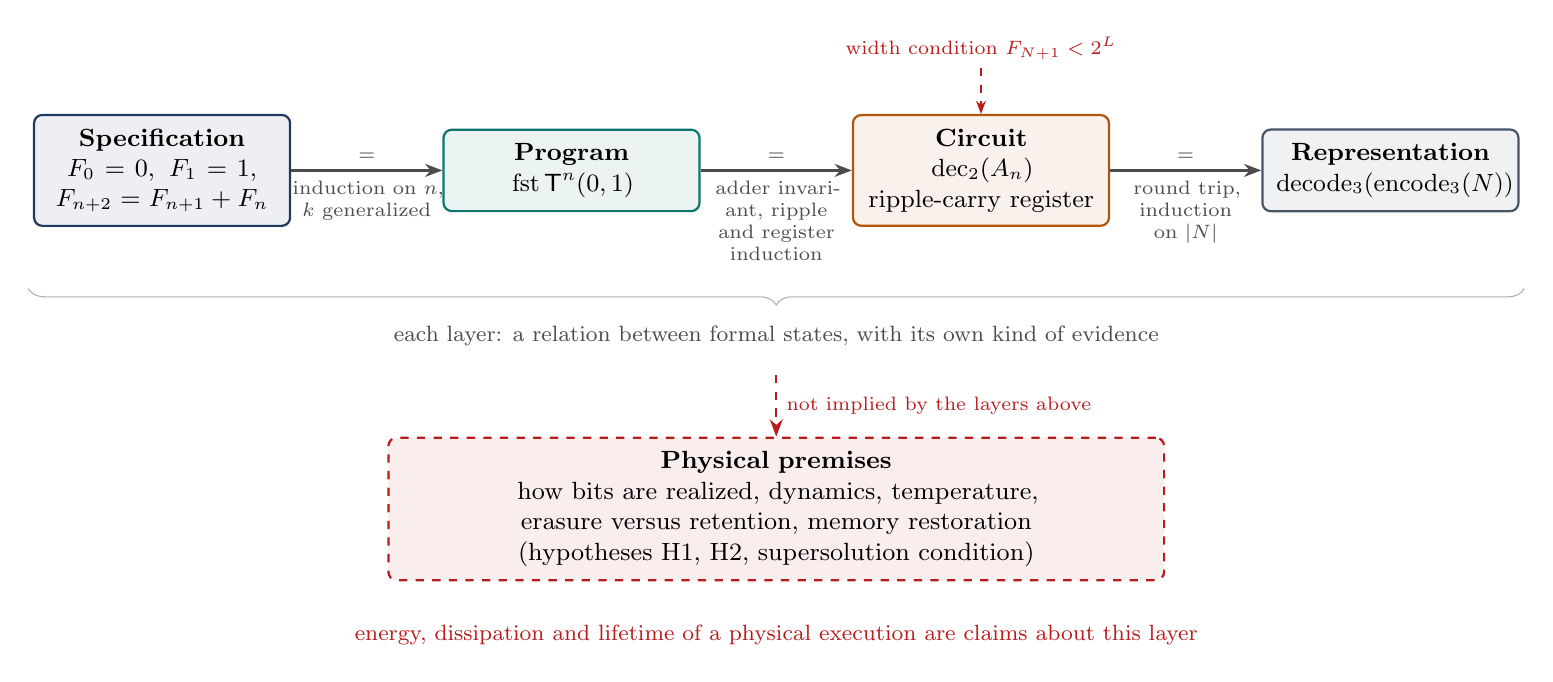
\begin{tikzpicture}[font=\small,>=Stealth,node distance=1cm]
\node[box=navy,text width=2.9cm] (S) at (0,0) {\textbf{Specification}\\ $F_0=0,\;F_1=1,$\\ $F_{n+2}=F_{n+1}+F_n$};
\node[box=teal,text width=2.9cm] (P) at (5.2,0) {\textbf{Program}\\ $\mathrm{fst}\,\mathsf T^{n}(0,1)$};
\node[box=amber,text width=2.9cm] (K) at (10.4,0) {\textbf{Circuit}\\ $\mathrm{dec}_2(A_n)$\\ ripple-carry register};
\node[box=slate,text width=2.9cm] (R) at (15.6,0) {\textbf{Representation}\\ $\mathrm{decode}_3(\mathrm{encode}_3(N))$};
\draw[arr=black!70] (S.east) -- node[above,font=\scriptsize,align=center]{$=$} node[below,font=\scriptsize,text width=1.9cm,align=center]{induction on $n$, $k$ generalized} (P.west);
\draw[arr=black!70] (P.east) -- node[above,font=\scriptsize]{$=$} node[below,font=\scriptsize,text width=1.9cm,align=center]{adder invariant, ripple and register induction} (K.west);
\draw[arr=black!70] (K.east) -- node[above,font=\scriptsize]{$=$} node[below,font=\scriptsize,text width=1.9cm,align=center]{round trip, induction on $|N|$} (R.west);
\node[font=\scriptsize,text=crimson,align=center] at (10.4,1.55) {width condition $F_{N+1}<2^{L}$};
\draw[crimson,dashed,->] (10.4,1.3) -- (K.north);
\draw[black!30,decorate,decoration={brace,amplitude=6pt,mirror}] (-1.7,-1.5) -- (17.3,-1.5);
\node[font=\footnotesize,text=black!70] at (7.8,-2.1) {each layer: a relation between formal states, with its own kind of evidence};
\node[box=crimson,text width=9.5cm,dashed] (X) at (7.8,-4.3) {\textbf{Physical premises}\\ how bits are realized, dynamics, temperature, erasure versus retention, memory restoration\\ (hypotheses H1, H2, supersolution condition)};
\draw[arr=crimson,dashed] (7.8,-2.6) -- node[right,font=\scriptsize,text=crimson]{not implied by the layers above} (X.north);
\node[font=\footnotesize,align=center,text=crimson] at (7.8,-5.9) {energy, dissipation and lifetime of a physical execution are claims about this layer};
\end{tikzpicture}
}
\caption{The four correctness layers and the physical premises. Each arrow is an equality between formal quantities established by a different kind of evidence, and the dashed arrow records that no claim about energy, dissipation or lifetime follows from the layers alone.}
\label{fig:layers}
\end{figure}

All four layers relate formal states: functions on integers, programs on pairs, bit-vectors in registers and digit strings. A verified numerical computation establishes that these relations hold. Claims about the energy, the dissipation or the lifetime of a physical execution of the computation require additional physical assumptions that none of the layers supplies: how bit values are realized, what dynamics moves them, at what temperature, which steps erase information and which retain it, and how the memory is restored. These are premises of the same kind as the hypotheses H1 and H2 and the supersolution condition of the earlier sections, and they play the same role, since the formal argument shows what follows from them and not that they hold. NAND universality and Church encodability alone establish no thermodynamic bound. Both are statements about expressiveness, and both hold equally for reversible gate sets used with ancillas, so they cannot determine a cost. The abstract map $\Tm$ is a bijection of $\mathbb{Z}^{2}$ with inverse $(x,y) \mapsto (y-x,\ x)$, is injective on $\mathbb{N}^{2}$ with its inverse defined on the image, where $y \ge x$, and has a fixed-width version $(a,b) \mapsto (b,\ (a+b) \bmod 2^{L})$ that is a bijection of $(\mathbb{Z}/2^{L}\mathbb{Z})^{2}$ with inverse $(x,y) \mapsto (y-x \bmod 2^{L},\ x)$, so the specified computation is logically reversible, while a circuit built from $\nand$ gates that discards its intermediate wires erases information. Which of these describes a physical execution is a property of the implementation and not of the specification. Representation also enters the accounting, since the unary, binary and balanced ternary encodings of the same value differ in size, and any resource claim must therefore name the representation as well as the function.

\section{Venn Diagrams and Directed Acyclic Graphs}
\label{sec:venn-dag}

The logical structures developed above admit two complementary graphical interpretations. Venn diagrams express relations among classes of objects or events, while directed acyclic graphs express dependencies among premises, computations and intermediate results. The first organizes membership and exclusion; the second organizes the order in which conclusions become available. Neither representation supplies missing premises, and neither converts an empirical assumption into a logical truth. Their usefulness lies in making different parts of the argument explicit, and in particular in showing which parts are structural, such as class inclusion, dependency order and acyclicity, and which are substantive, such as the measure, the inference rules and the supersolution. A diagram supports an inference only when its syntax, semantics and transformation rules are explicit, and diagrammatic representations can themselves constitute formal proof systems when those rules are specified and their soundness is established \cite{shin1995}.

\subsection{Class Inclusion and the Syllogism}

Let $\mathrm{Person}$ be the domain of persons and define the subsets
\[
\llbracket\mathrm{Man}\rrbracket=\{x\in\mathrm{Person}:\mathrm{Man}(x)\},
\qquad
\llbracket\mathrm{Mortal}\rrbracket=\{x\in\mathrm{Person}:\mathrm{Mortal}(x)\}.
\]
The universal premise that all men are mortal becomes the inclusion
\[
\llbracket\mathrm{Man}\rrbracket\subseteq\llbracket\mathrm{Mortal}\rrbracket,
\]
and the instance premise becomes $\mathrm{socrates}\in\llbracket\mathrm{Man}\rrbracket$. The conclusion follows by membership transport:
\[
\mathrm{socrates}\in\llbracket\mathrm{Man}\rrbracket
\quad\text{and}\quad
\llbracket\mathrm{Man}\rrbracket\subseteq\llbracket\mathrm{Mortal}\rrbracket
\quad\Longrightarrow\quad
\mathrm{socrates}\in\llbracket\mathrm{Mortal}\rrbracket.
\]
An Euler diagram represents the inclusion by placing the region $\llbracket\mathrm{Man}\rrbracket$
inside the region $\llbracket\mathrm{Mortal}\rrbracket$. A strict Venn diagram instead displays all
membership combinations and marks $\llbracket\mathrm{Man}\rrbracket\cap\llbracket\mathrm{Mortal}\rrbracket^{c}$ as empty. Both
representations express the same premise, although they do so by
different graphical conventions.

The corresponding proof term,
\[
\mathrm{all\_men\_mortal}\;
\mathrm{socrates}\;
\mathrm{socrates\_man},
\]
performs the membership transport that the diagram displays. The
diagram does not establish that the region $\llbracket\mathrm{Man}\rrbracket\cap\llbracket\mathrm{Mortal}\rrbracket^{c}$ is actually
empty in the world. That exclusion is the universal premise itself.
It also does not specify when a mortal person dies, because a class
inclusion contains no distribution over lifetimes. A temporal or
probabilistic reading requires the additional process model introduced
in the mortality argument.

\subsection{Boolean Operations as Operations on Regions}

Fix a universe $U$. Under a classical interpretation, a proposition
depending on an assignment determines the subset of assignments on
which it is true. If propositions $A$ and $B$ determine regions
$\llbracket A\rrbracket$ and $\llbracket B\rrbracket$, then
\[
\llbracket A\land B\rrbracket
=\llbracket A\rrbracket\cap\llbracket B\rrbracket,
\qquad
\llbracket A\lor B\rrbracket
=\llbracket A\rrbracket\cup\llbracket B\rrbracket,
\]
and
\[
\llbracket\neg A\rrbracket
=U\setminus\llbracket A\rrbracket.
\]
Material implication is represented by
\[
\llbracket A\to B\rrbracket
=
\big(U\setminus\llbracket A\rrbracket\big)
\cup\llbracket B\rrbracket.
\]
Consequently, $A\to B$ is true on every assignment exactly when
$\llbracket A\rrbracket\subseteq\llbracket B\rrbracket$.
These are Boolean truth conditions; they do not by themselves
represent the evidence carried by a constructive proof of an
implication.

The NAND operation has the regional interpretation
\[
\llbracket A\nand B\rrbracket
=
U\setminus
\big(\llbracket A\rrbracket\cap\llbracket B\rrbracket\big).
\]
Its functional completeness can therefore be read geometrically:
complemented intersection suffices to construct complement,
intersection and union, and hence every Boolean combination of a
finite collection of regions. This is the set-theoretic counterpart
of the NAND identities proved above. The construction concerns which
regions can be specified, rather than the number of gates, the time
required to evaluate them or the energy consumed by their physical
implementation.

\subsection{Event Inclusion and Exponential Bounds}

The probabilistic proofs also contain inclusions that can be
represented by overlapping regions, provided the universe is now a
space of trajectories equipped with a probability measure. Under H2,
at each cycle boundary,
\[
\{E_n\ge w\}
\subseteq
\{Z_n\ge e^{\beta w-\kappa}\}.
\]
Taking the union over all cycle counts preserves inclusion:
\[
\bigcup_{n\ge0}\{E_n\ge w\}
\subseteq
\bigcup_{n\ge0}
\{Z_n\ge e^{\beta w-\kappa}\}.
\]
The first region consists of trajectories on which the engine
eventually reaches the work threshold. The second consists of
trajectories on which the exponential process reaches the
corresponding level. H2 establishes the containment, while H1
permits Ville's inequality to bound the probability measure of the
containing region.

A Venn diagram can display this containment but cannot establish
the exponential estimate from its drawn areas. Probability is
supplied by the measure, and the estimate is supplied by the
supermartingale theorem. A small region on the page need not have
small probability unless the drawing has been constructed to
represent that measure. The distinction parallels the difference
between a class inclusion and an empirical claim about how many
objects occupy each class.

\subsection{Proofs and Computations as Dependency Graphs}

A directed acyclic graph represents a different structure. Its
vertices denote premises, intermediate results or computations, and
an edge indicates that one vertex is used in obtaining another.
Acyclicity permits a topological ordering in which every dependency
is available before the result that uses it \cite[Section~20.4]{cormen2022}. For a proof, the
vertices must also record the inference rules that justify their
conclusions: the existence of an edge alone does not establish a
valid inference.

The Socrates proof has one application step depending jointly on
the universal premise and the instance premise. Those dependencies
are conjunctive: both are required. An ordinary graph records the
dependencies, while a labeled inference vertex or a directed
hyperedge, which is an edge with several sources and one target, records that they jointly support the conclusion.
Alternative proofs require a further distinction between several
premises needed together and several independently sufficient
routes to the same result.

The Fibonacci computation gives a larger example. Introduce one
vertex for each value $F_k$, and for every $k\ge2$ draw dependency
edges from $F_{k-1}$ and $F_{k-2}$ to $F_k$. The resulting graph has
only $n+1$ value vertices through index $n$. The naive recursive
program unfolds this graph into a call tree, duplicating a
subproblem whenever it is encountered again. Memoization retains
one result per vertex, while the rolling-state implementation keeps
only the two values needed at the current boundary between completed
and pending work. Dynamic programming exploits the dependency graph;
the accumulator exploits the limited amount of that graph that must
remain available.

The NAND full adder has the same graphical character. Its shared
intermediates $u$, $p$ and $v$ are vertices whose output wires feed
several later gates. Expanding every use into a separate expression
produces a formula tree, whereas retaining shared vertices gives a
circuit graph. A topological evaluation of that graph computes each
gate after its inputs are available. The local invariant
$a+b+c_{\mathrm{in}}=s+2c_{\mathrm{out}}$ supplies the arithmetic meaning of the resulting
outputs; acyclicity alone supplies only a permissible evaluation
order.

\subsection{Time Expansion and Bellman Recursion}

A physical process need not have an acyclic state-transition graph.
An active state may be revisited, an engine may return to its initial
configuration, and a register may repeatedly execute the same
transition. A finite-horizon computation nevertheless has an
acyclic representation when time or remaining horizon is included
in each vertex.

\begin{figure}[tbp]
\centering
\resizebox{\textwidth}{!}{%
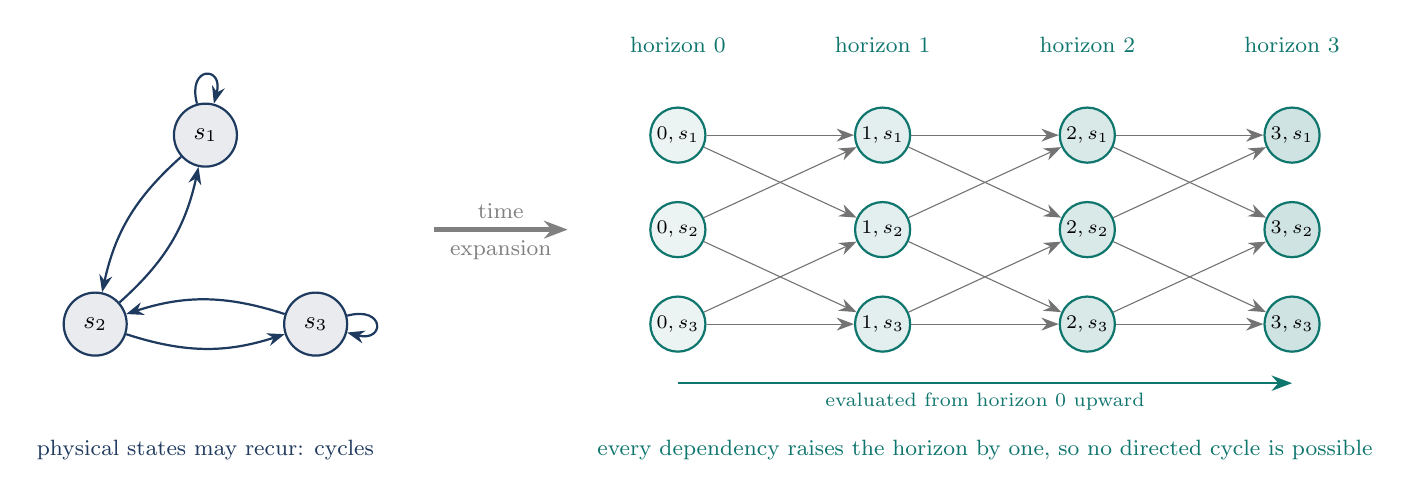
\begin{tikzpicture}[font=\small,>=Stealth]
\node[circle,draw=navy,fill=navy!10,thick,minimum size=8mm] (p1) at (0,1.6) {$s_1$};
\node[circle,draw=navy,fill=navy!10,thick,minimum size=8mm] (p2) at (-1.4,-0.8) {$s_2$};
\node[circle,draw=navy,fill=navy!10,thick,minimum size=8mm] (p3) at (1.4,-0.8) {$s_3$};
\draw[arr=navy] (p1) to[loop above,looseness=6] (p1);
\draw[arr=navy] (p1) to[bend right=18] (p2); \draw[arr=navy] (p2) to[bend right=18] (p1);
\draw[arr=navy] (p2) to[bend right=18] (p3); \draw[arr=navy] (p3) to[bend right=18] (p2);
\draw[arr=navy] (p3) to[loop right,looseness=6] (p3);
\node[font=\footnotesize,text=navy,align=center] at (0,-2.4) {physical states may recur: cycles};
\draw[-{Stealth[length=3mm]},line width=1.6pt,black!50] (2.9,0.4) -- node[above,font=\footnotesize]{time} node[below,font=\footnotesize]{expansion} (4.6,0.4);
\node[circle,draw=teal,fill=teal!8,thick,minimum size=7mm,font=\scriptsize,inner sep=0pt] (v01) at (6.00,1.60) {$0,s_1$};
\node[circle,draw=teal,fill=teal!8,thick,minimum size=7mm,font=\scriptsize,inner sep=0pt] (v02) at (6.00,0.40) {$0,s_2$};
\node[circle,draw=teal,fill=teal!8,thick,minimum size=7mm,font=\scriptsize,inner sep=0pt] (v03) at (6.00,-0.80) {$0,s_3$};
\node[font=\footnotesize,text=teal] at (6.00,2.75) {horizon $0$};
\node[circle,draw=teal,fill=teal!12,thick,minimum size=7mm,font=\scriptsize,inner sep=0pt] (v11) at (8.60,1.60) {$1,s_1$};
\node[circle,draw=teal,fill=teal!12,thick,minimum size=7mm,font=\scriptsize,inner sep=0pt] (v12) at (8.60,0.40) {$1,s_2$};
\node[circle,draw=teal,fill=teal!12,thick,minimum size=7mm,font=\scriptsize,inner sep=0pt] (v13) at (8.60,-0.80) {$1,s_3$};
\node[font=\footnotesize,text=teal] at (8.60,2.75) {horizon $1$};
\node[circle,draw=teal,fill=teal!16,thick,minimum size=7mm,font=\scriptsize,inner sep=0pt] (v21) at (11.20,1.60) {$2,s_1$};
\node[circle,draw=teal,fill=teal!16,thick,minimum size=7mm,font=\scriptsize,inner sep=0pt] (v22) at (11.20,0.40) {$2,s_2$};
\node[circle,draw=teal,fill=teal!16,thick,minimum size=7mm,font=\scriptsize,inner sep=0pt] (v23) at (11.20,-0.80) {$2,s_3$};
\node[font=\footnotesize,text=teal] at (11.20,2.75) {horizon $2$};
\node[circle,draw=teal,fill=teal!20,thick,minimum size=7mm,font=\scriptsize,inner sep=0pt] (v31) at (13.80,1.60) {$3,s_1$};
\node[circle,draw=teal,fill=teal!20,thick,minimum size=7mm,font=\scriptsize,inner sep=0pt] (v32) at (13.80,0.40) {$3,s_2$};
\node[circle,draw=teal,fill=teal!20,thick,minimum size=7mm,font=\scriptsize,inner sep=0pt] (v33) at (13.80,-0.80) {$3,s_3$};
\node[font=\footnotesize,text=teal] at (13.80,2.75) {horizon $3$};
\draw[arr=black!55,thin] (v01) -- (v11);
\draw[arr=black!55,thin] (v02) -- (v11);
\draw[arr=black!55,thin] (v01) -- (v12);
\draw[arr=black!55,thin] (v03) -- (v12);
\draw[arr=black!55,thin] (v02) -- (v13);
\draw[arr=black!55,thin] (v03) -- (v13);
\draw[arr=black!55,thin] (v11) -- (v21);
\draw[arr=black!55,thin] (v12) -- (v21);
\draw[arr=black!55,thin] (v11) -- (v22);
\draw[arr=black!55,thin] (v13) -- (v22);
\draw[arr=black!55,thin] (v12) -- (v23);
\draw[arr=black!55,thin] (v13) -- (v23);
\draw[arr=black!55,thin] (v21) -- (v31);
\draw[arr=black!55,thin] (v22) -- (v31);
\draw[arr=black!55,thin] (v21) -- (v32);
\draw[arr=black!55,thin] (v23) -- (v32);
\draw[arr=black!55,thin] (v22) -- (v33);
\draw[arr=black!55,thin] (v23) -- (v33);
\node[font=\footnotesize,text=teal,align=center] at (9.9,-2.4) {every dependency raises the horizon by one, so no directed cycle is possible};
\draw[-{Stealth[length=2.6mm]},thick,teal] (6.0,-1.55) -- node[below,font=\scriptsize]{evaluated from horizon $0$ upward} (13.8,-1.55);
\end{tikzpicture}
}
\caption{Time expansion of a recurrent state graph. Physical states $s_1, s_2, s_3$ may recur (left), but the dependency graph on pairs of horizon and state is acyclic because every dependency raises the horizon by one (right). The transition structure is illustrative.}
\label{fig:bellman}
\end{figure}

For the Bellman recursion, a vertex $(n+1,s,z)$ depends on
continuation vertices $(n,s',z-r)$. Every dependency reduces the
remaining horizon by one, so a directed cycle is impossible even
when the physical state $s$ can recur. In a finite model the part of this graph reachable from a fixed initial state, target and horizon is finite, although the collection of vertices over all real targets is not, and it is evaluated from horizon zero upward. The
corresponding survival recursion has vertices $(n,s)$ and the same
decrease of horizon along dependencies.

This time expansion also clarifies why an inductive hypothesis must
cover every reachable continuation state. After a transition, the
computation refers to a different vertex, with a changed state and a
shorter horizon. The generalized invariant guarantees that the
required assertion is available there. For the work-threshold
problem, the exponential supersolution bounds every such
continuation and remains valid under the maximization over
admissible actions. The graph records the recursion's dependencies;
the supersolution proves the bound propagated through them.

These dependency graphs should be distinguished from causal graphs
and Bayesian networks. A computational edge records use of a value,
whereas a causal edge asserts a relation within a causal model.
Interpreting a graph as a Bayesian network requires specified
conditional distributions and a factorization assumption.
Likewise, a proof graph requires inference rules. The shared
graphical form does not make these interpretations interchangeable.

Venn diagrams and directed acyclic graphs therefore expose
complementary aspects of the essay's arguments. Regional diagrams
display class relations, Boolean operations and event inclusions.
Dependency graphs display the premises and intermediate results
needed to derive or compute a conclusion. In both cases the
representation helps locate the correctness obligation, while the
proof rules, probability measure and physical assumptions remain
responsible for satisfying it.

\section{Closed Derivations and Accountable Models}\label{sec:accountable}

A methodological point that the preceding layers leave implicit can be made through an example from media theory. Baudrillard's discussion of Disneyland \cite{baudrillard1994}, presented in a recent video lecture \cite{academicagent2026}, argues that an enclosure announced as imaginary invites visitors to treat the surrounding world as the unconstructed baseline, whereas the surroundings are themselves organized through signs, scripts and managed expectations that are simply less conspicuous. The strong form of the thesis, on which representations refer to nothing outside the system of representations, is not needed here and is not adopted. Two propositions must be kept apart: that an event is mediated, meaning that it becomes recognizable and significant through established references, and that it has no referent beyond its representation. The first does not entail the second. A news cycle can become preoccupied with reactions to reactions while the original event retains material causes and consequences, and learning of something through a report does not make its existence depend on the report. If circulating representations alter appointments, policies or conduct, their circulation is causally connected to the world even when it distorts what happened.

What the example contributes is a distinction between two kinds of closed system. A formal system receives its interpretation through an explicitly stated semantics, and its internal transformations can be checked against that interpretation: a Church numeral denotes an iteration count, a $\nand$ circuit denotes a Boolean function, and the correctness statements of the preceding section are statements about the agreement of these readings. A system of circulating signs becomes epistemically troublesome when its internal measures of success, such as recognition, repetition and engagement, displace checks against what its claims concern, so that internal consistency and circulation substitute for external correction. Self-reference alone does not establish this failure, since mathematical proofs also refer to other proofs and remain accountable to definitions and rules of inference. The failure lies in the loss of a channel through which contrary evidence could change the conclusion.

The thermodynamic argument of this essay exhibits the formal analogue. A derivation from the hypotheses H1 and H2, or from the supersolution condition, is a closed derivation: its conclusion is a theorem relative to the hypotheses, and it announces its conventions in the way the enclosure announces itself as imaginary. The idealizations it contains, such as a reservoir held at fixed temperature, a work-storage system of unchanged entropy and a memory restored to a standard state, are the analogue of the surroundings that go unremarked when the model is applied. The risk is the one the example identifies, and it is the treatment of the application as the unmodeled baseline. Let $C$ be the claim that the probability law of a particular physical engine satisfies the exponential bound and $\mathcal{H}$ the conjunction of the hypotheses for that engine, and let $\Pr$ denote credence over which physical model applies (the third use in Definition~\ref{def:prob}), with $0 < \Pr(\mathcal{H}) < 1$ so that both conditional probabilities are defined. The derivation establishes $\mathcal{H} \Rightarrow C$ within the model, hence $\Pr(C \mid \mathcal{H}) = 1$, and then
\[
\Pr(C) \;=\; \Pr(C \mid \mathcal{H})\,\Pr(\mathcal{H}) + \Pr(C \mid \neg \mathcal{H})\,\Pr(\neg \mathcal{H}) \;\ge\; \Pr(\mathcal{H}),
\]
where the lower bound uses only the theorem. The derivation fixes the first factor and says nothing about $\Pr(\mathcal{H})$ or about $\Pr(C \mid \neg \mathcal{H})$, and both of these are matters of evidence about the actual engine, namely whether the dynamics is reversible, whether the protocol is independent of the microstate, and whether the boundary term is bounded. The distinction matters because uncertainty about which model applies, recorded by $\Pr(\mathcal{H})$, differs from fluctuation within a fixed model, which the bound itself accounts for. If $C$ instead meant that an individual run stays below a threshold, the theorem would give only a probability bound for that event and not $\Pr(C \mid \mathcal{H}) = 1$. This is the same division as in the syllogism, where the inference is certain and the credence attaches to the premises, and it is the reason that a reported working engine is treated as evidence against a hypothesis and not as a refutation of the theorem.

The corresponding question for any circulating account, formal or informal, concerns its channels of correction. One may ask what evidence could correct it, which distinctions its presentation suppresses, and whether contrary observations can change its conclusions. A formally closed derivation answers the third question by exposing its hypotheses as the places where contrary observation applies. An account that cannot say which observation would count against it has become closed in the unhelpful sense, even if every inference within it is valid. The comparison also bounds what the Disneyland example can show. It supports the methodological claim that conventions of presentation shape what appears to need justification, and it does not support the stronger claim that mediated reality has lost every external referent, since the engine bounds above are accountable to measurable quantities and the layered correctness proofs are accountable to definitions that can be checked.

\section{Comparison of the Four Readings}

The four interpretations agree at the level of the exponential and differ in what they take as primitive. The combinatorial reading takes the microstate count as primitive and yields a pigeonhole bound on one cycle, with the asymmetry of time supplied by the choice of initial measure. The stochastic reading takes the trajectory ensemble as primitive and yields a time-uniform bound through a martingale. The Bayesian reading takes the state of knowledge as primitive and yields an average-work bound by an accounting identity in which information, correlations and nonequilibrium free energy enter a resource balance under specified conditions. The dynamic programming reading takes the controlled transition kernel as primitive and shows that the martingale bound is a Bellman supersolution. The readings differ in logical form as well as in primitives. The combinatorial bound is a bound on the fraction of initial microstates, under the uniform measure on a starting macrostate, that produce one cycle of the behavior. The stochastic bound is a time-uniform bound on a probability of ever reaching a given extracted work, valid under H1 and H2. The Bayesian result is a bound on average work obtained from an accounting identity, valid for an idealized memory. The dynamic programming result is a probability bound over all admissible policies, valid when the supersolution condition holds for every action. None of them is simply stronger than the others, since they bound different quantities. The combinatorial bound is on a fraction of initial microstates, the stochastic and dynamic programming bounds are on probabilities of reaching a threshold, and the Bayesian result is on an average. The stochastic theorem does establish, under H1 and H2, that unbounded cumulative extraction has probability zero, while finite work-extracting fluctuations remain possible. An event of probability zero in a model is not a logically contradictory event, and none of the results proves that a work-extracting fluctuation cannot occur.

The book \emph{The Mortality of Computation} \cite{flyxion2026} reaches the neighboring conclusion from the side of computation: universality is formal while finitude is physical, so that, in the book's terms, a running program is a metastable process, and when the cumulative lower bound on the energy it must transfer to its surroundings eventually exceeds a finite energy budget, the number of irreversible operations it can perform is bounded. The book is used here only for its stated thesis, and its own results, many of which it labels heuristic, are not relied upon. The engine bounds above are a quantitative analogue of that claim for a thermal device, not a derivation of it, and the contrast with the syllogism applies to both, since the logical term is timeless while the physical process that carries it out is not.

The relation to the proof-assistant techniques is organizational and should not be mistaken for an explanation. Generalization of the carried quantity corresponds to quantifying over the starting state, whether that is the pair of Fibonacci numbers, the active state of the organism, or the microstate of the engine. The one-step lemma corresponds to the single-cycle identity, the fluctuation relation, or the Markov step of the survival chain. Transport along an equality of indices is, in the Fibonacci proof and in the survival proof (where $jm + m = (j+1)m$), a matter of arithmetic. In the thermodynamic argument the corresponding step, passing from cycles to elapsed time, needs a model of cycle duration and is not mere rewriting. In the account developed here the asymmetry between the two directions of time enters through the choice of initial measure and the coarse-graining, which is one standard view that is not argued for here against alternatives in the foundations of statistical mechanics, and the proof-assistant techniques only keep track of which premises each conclusion uses. The syllogism has none of these steps because its conclusion is obtained at the first.

\section{Limits of the Argument}

Beyond the non-claims of Section~\ref{sec:terms}, several limits should be stated plainly. The martingale bound rests on hypotheses H1 and H2, which must be verified for a given driven model. Quantum devices introduce measurement and coherence effects that the classical derivation does not cover, and with two reservoirs at different temperatures extraction is ordinary and is simply a heat engine. The feedback accounting is idealized as stated in the Bayesian section, and a demon whose memory remains correlated with the system is a case the argument does not close. The combinatorial bound presupposes a finite microstate set and a uniform initial measure, and it does not say why that measure is the right one; the stochastic and Bellman results are for finite models. The mortality model is a premise about what viability requires and not a result of physics, and repair defeats the result only if it defeats the uniform block mortality condition, which is why the mortality claim and the engine claim are not equally secure. The resource counts of the computational thread are for the specific algorithms and circuits described and are not lower bounds on the problems they solve. Results quoted from the literature should be consulted at their sources for their exact hypotheses.

\section{Conclusion}

Socrates is mortal by a single application of a universal premise, and the argument has nothing to say about whether the premise is true. The essay does not show that a perpetual motion machine of the second kind is impossible. It shows, in the following precise sense, that extraction is bounded under stated hypotheses. The combinatorial model bounds a specified transition. The stochastic theorem excludes unbounded cumulative extraction almost surely under H1 and H2, and the dynamic programming formulation extends this to all admissible policies when the supersolution condition holds for each action. The feedback accounting bounds average work once the information resources are included. These results follow from reversibility together with a probability model, whether the measure is read as a count, an ensemble or a state of knowledge, and the Bellman recursion is built upon that model and is not itself a probability measure. Each result answers to its own hypotheses. The computational thread supports the same moral at the level of implementation: a specification, a program, a circuit and a representation are four separate claims with four kinds of evidence, and a verified numerical computation relates formal states without fixing the energy, dissipation or lifetime of its physical execution. The two conclusions share the structure of conclusions conditional on premises, with premises of different epistemic status, and the techniques that organize a proof about an accumulator, namely generalizing the carried state, proving the step for all states, and transporting along index equalities, serve to separate the part of each argument that is certain from the part that is a hypothesis about the world.

\appendix

\section{Supermartingales, Stopping and Ville's Inequality}\label{app:martingale}

Let $(\Omega, \mathcal{G}, \Pr)$ be a probability space with a filtration $(\mathcal{G}_n)_{n \ge 0}$. A process $(Z_n)$ is a supermartingale if it is adapted, each $Z_n$ is integrable, and $\E[Z_{n+1} \mid \mathcal{G}_n] \le Z_n$ almost surely. A stopping time is a random variable $\tau$ with values in $\mathbb{N} \cup \{\infty\}$ such that $\{\tau \le n\} \in \mathcal{G}_n$ for every $n$.

\begin{lemma}[Stopped supermartingale]\label{lem:stopped}
If $(Z_n)$ is a supermartingale and $\tau$ is a stopping time, then $N_n = Z_{\tau \wedge n}$ is a supermartingale, and in particular $\E[Z_{\tau \wedge n}] \le \E[Z_0]$ for every $n$.
\end{lemma}

\begin{proof}
On $\{\tau \le n\}$ we have $N_{n+1} = N_n = Z_\tau$, and on $\{\tau > n\}$ we have $N_{n+1} = Z_{n+1}$ and $N_n = Z_n$. Hence $N_{n+1} - N_n = \mathbf{1}_{\{\tau > n\}}(Z_{n+1} - Z_n)$. The event $\{\tau > n\}$ is the complement of $\{\tau \le n\}$ and lies in $\mathcal{G}_n$, so
\[
\E[N_{n+1} - N_n \mid \mathcal{G}_n] = \mathbf{1}_{\{\tau > n\}}\big(\E[Z_{n+1} \mid \mathcal{G}_n] - Z_n\big) \le 0 .
\]
Integrability holds because $|N_n| \le \sum_{k \le n} |Z_k|$. Taking expectations gives $\E[N_n] \le \E[N_0] = \E[Z_0]$.
\end{proof}

\begin{proposition}[Ville's maximal inequality]\label{prop:villeapp}
If $(Z_n)$ is a nonnegative supermartingale and $\lambda > 0$, then $\Pr(\exists\, n : Z_n \ge \lambda) \le \E[Z_0]/\lambda$, and consequently $\Pr(\sup_n Z_n \ge \lambda) \le \E[Z_0]/\lambda$.
\end{proposition}

\begin{proof}
Let $\tau = \inf\{n : Z_n \ge \lambda\}$. For each $N$, Lemma~\ref{lem:stopped} and nonnegativity give
\[
\E[Z_0] \ge \E[Z_{\tau \wedge N}] \ge \E\big[Z_\tau \mathbf{1}_{\{\tau \le N\}}\big] \ge \lambda\,\Pr(\tau \le N),
\]
where the middle inequality drops the nonnegative contribution of $\{\tau > N\}$. Letting $N \to \infty$ and using continuity of probability from below, $\Pr(\tau < \infty) \le \E[Z_0]/\lambda$. For the supremum, $\{\sup_n Z_n \ge \lambda\} \subseteq \{\exists\, n : Z_n \ge \lambda'\}$ for every $\lambda' < \lambda$, so the probability is at most $\E[Z_0]/\lambda'$ for every such $\lambda'$ and hence at most $\E[Z_0]/\lambda$.
\end{proof}

\begin{corollary}\label{cor:villeone}
If in addition $Z_0 = 1$, then $\Pr(\exists\, n : Z_n \ge \lambda) \le \min\{1, 1/\lambda\}$. If $E_n \ge w$ implies $Z_n \ge e^{\beta w - \kappa}$ for every $n$, then $\Pr(\exists\, n : E_n \ge w) \le \min\{1, e^{\kappa - \beta w}\}$.
\end{corollary}

The inequality concerns the whole trajectory at once. A fixed-time bound controls $\Pr(Z_n \ge \lambda)$ for one prescribed $n$ and says nothing about the first crossing time, whereas Proposition~\ref{prop:villeapp} controls the event that the level is crossed at some time, which is the event relevant to adaptive stopping rules. This distinction is used in Appendix~\ref{app:popular}.

\section{A Discrete-Time Derivation of the Crooks Relation}\label{app:crooks}

This appendix derives the relation assumed in the stochastic section for a finite, discrete-time, driven Markov model, so that its hypotheses are explicit. Let $\mathcal{X}$ be a finite set, let $U_0, \dots, U_T : \mathcal{X} \to \mathbb{R}$ be energy functions, and write
\[
\rho_t(x) = e^{-\beta (U_t(x) - f_t)}, \qquad f_t = -\beta^{-1} \ln \sum_{x} e^{-\beta U_t(x)},
\]
so that $\rho_t$ is the canonical distribution and $f_t$ the equilibrium free energy of $U_t$. Let $K_1, \dots, K_T$ be stochastic matrices on $\mathcal{X}$ satisfying detailed balance with respect to $\rho_t$, meaning $\rho_t(x) K_t(x,y) = \rho_t(y) K_t(y,x)$. The forward protocol draws $x_0 \sim \rho_0$ and, for $t = 0, \dots, T-1$, first switches the energy from $U_t$ to $U_{t+1}$ with the state held fixed, and then draws $x_{t+1} \sim K_{t+1}(x_t, \cdot)$. The work and heat in step $t$ are
\[
w_t = U_{t+1}(x_t) - U_t(x_t), \qquad q_t = U_{t+1}(x_{t+1}) - U_{t+1}(x_t),
\]
and with $W = \sum_t w_t$ and $Q = \sum_t q_t$ the first law reads $U_T(x_T) - U_0(x_0) = W + Q$. The forward path probability is
\[
P_F(x_0, \dots, x_T) = \rho_0(x_0) \prod_{t=0}^{T-1} K_{t+1}(x_t, x_{t+1}).
\]
The reversed protocol draws $x_T \sim \rho_T$, evolves by $K_T$ from $x_T$ to $x_{T-1}$, switches the energy from $U_T$ to $U_{T-1}$, and continues in this way down to $x_0$, so its path probability on the reversed path $\tilde{x} = (x_T, \dots, x_0)$ is
\[
P_R(\tilde{x}) = \rho_T(x_T) \prod_{t=0}^{T-1} K_{t+1}(x_{t+1}, x_t).
\]

\begin{proposition}[Crooks relation]\label{prop:crooksapp}
If $P_F(x) > 0$ then $P_R(\tilde{x}) > 0$, and
\[
\frac{P_F(x)}{P_R(\tilde{x})} = \exp\big(\beta\,(W(x) - \Delta F)\big), \qquad \Delta F = f_T - f_0 .
\]
\end{proposition}

\begin{proof}
Detailed balance with $\rho_{t+1} > 0$ gives $K_{t+1}(x_{t+1}, x_t) > 0$ whenever $K_{t+1}(x_t, x_{t+1}) > 0$, so $P_R(\tilde x) > 0$. The ratio is
\[
\frac{P_F(x)}{P_R(\tilde{x})} = \frac{\rho_0(x_0)}{\rho_T(x_T)} \prod_{t=0}^{T-1} \frac{K_{t+1}(x_t, x_{t+1})}{K_{t+1}(x_{t+1}, x_t)} = \frac{\rho_0(x_0)}{\rho_T(x_T)} \prod_{t=0}^{T-1} \frac{\rho_{t+1}(x_{t+1})}{\rho_{t+1}(x_t)},
\]
by detailed balance. By the definition of $\rho_{t+1}$, the product equals $\exp\big(-\beta \sum_t [U_{t+1}(x_{t+1}) - U_{t+1}(x_t)]\big) = e^{-\beta Q}$, and
\[
\frac{\rho_0(x_0)}{\rho_T(x_T)} = \exp\big(\beta [U_T(x_T) - U_0(x_0)] - \beta (f_T - f_0)\big) = e^{\beta (W + Q) - \beta \Delta F}.
\]
Multiplying, the heat cancels and the ratio is $e^{\beta (W - \Delta F)}$.
\end{proof}

\begin{corollary}[Jarzynski identity and tail bound]\label{cor:jarzapp}
Under the forward protocol, $\E_F[e^{-\beta (W - \Delta F)}] = 1$. For a cycle, meaning $U_T = U_0$, one has $\Delta F = 0$, and for every $w \ge 0$, $\Pr_F(W \le -w) \le e^{-\beta w}$.
\end{corollary}

\begin{proof}
By Proposition~\ref{prop:crooksapp}, $P_F(x) e^{-\beta (W(x) - \Delta F)} = P_R(\tilde{x})$ on the support of $P_F$. A reversed path $\tilde x$ has $P_R(\tilde x) > 0$ exactly when every $K_{t+1}(x_{t+1}, x_t) > 0$, which by detailed balance is equivalent to every $K_{t+1}(x_t, x_{t+1}) > 0$, so $x \mapsto \tilde{x}$ is a bijection from the support of $P_F$ onto the support of $P_R$. Summing gives $\sum_x P_R(\tilde x) = 1$. For the tail, on $\{W \le -w\}$ the nonnegative variable $e^{-\beta W}$ is at least $e^{\beta w}$, and Markov's inequality with $\E[e^{-\beta W}] = 1$ gives the bound.
\end{proof}

The hypotheses are visible in the derivation: each kernel is in detailed balance with the instantaneous canonical distribution, the work is done in instantaneous energy switches, and the initial state is canonical. Dynamics that violate any of these require a separate argument.

\section{The Stationary Entropy-Production Martingale}\label{app:stationary}

Let $K$ be a stochastic matrix on a finite set $\mathcal{X}$ with a stationary distribution $\nu$, so that $\sum_y \nu(y) K(y,x) = \nu(x)$, with $\nu(x) > 0$ for all $x$ and with symmetric support, meaning $K(x,y) > 0$ if and only if $K(y,x) > 0$. Start the chain from $x_0 \sim \nu$ and define the entropy production of the path $(x_0, \dots, x_n)$ by comparison with its reversal,
\[
\Sigma_n = \ln \frac{\nu(x_0) \prod_{t<n} K(x_t, x_{t+1})}{\nu(x_n) \prod_{t<n} K(x_{t+1}, x_t)} .
\]

\begin{proposition}\label{prop:stationary}
The process $e^{-\Sigma_n}$ is a martingale with respect to the natural filtration, with $\E[e^{-\Sigma_n}] = 1$. Without the symmetric-support assumption it is a supermartingale.
\end{proposition}

\begin{proof}
The one-step ratio is $e^{-\Sigma_{n+1}}/e^{-\Sigma_n} = \nu(x_{n+1}) K(x_{n+1}, x_n) / \big(\nu(x_n) K(x_n, x_{n+1})\big)$. Conditioning on $x_n = x$,
\[
\E\!\left[\frac{e^{-\Sigma_{n+1}}}{e^{-\Sigma_n}} \,\Big|\, x_n = x\right] = \sum_{y : K(x,y) > 0} K(x,y)\, \frac{\nu(y) K(y,x)}{\nu(x) K(x,y)} = \frac{1}{\nu(x)} \sum_{y : K(x,y) > 0} \nu(y) K(y,x) .
\]
Under symmetric support the sum may be taken over all $y$, since terms with $K(x,y) = 0$ have $K(y,x) = 0$, and stationarity gives $\sum_y \nu(y) K(y,x) = \nu(x)$, so the conditional expectation is $1$. Without symmetric support the sum is over a subset of nonnegative terms, so it is at most $1$.
\end{proof}

\begin{remark}
If $K$ is reversible with respect to $\nu$, then $\nu(x) K(x,y) = \nu(y) K(y,x)$ and the numerator and denominator of $\Sigma_n$ coincide, so $\Sigma_n \equiv 0$. An equilibrium chain has zero entropy production, and the proposition is informative only for chains with nonzero probability currents. The proposition also does not identify $\Sigma_n$ with thermodynamic entropy production for a driven protocol, which is the content that H1 asserts for driven models and which has to be established for the model at hand.
\end{remark}

\section{The Bellman Principle and the Supersolution Bound in the Finite Model}\label{app:bellman}

The model is finite: a finite state set $S$, a finite nonempty action set $A(s)$ at each state, a finite set $R \subset \mathbb{R}$ of work increments, and for each $(s,a)$ a probability distribution $K(\cdot, \cdot \mid s, a)$ on $S \times R$. A policy $\pi$ is a sequence of maps from histories $(s_0, a_0, r_0, \dots, s_n)$ to probability distributions on $A(s_n)$. Under $\pi$ and initial state $s_0$ the process has law $\Pr^\pi_{s_0}$. Write $E_n = \sum_{i<n} r_i$ and, for a target $z \in \mathbb{R}$, $\tau_z = \inf\{n \ge 0 : E_n \ge z\}$, so $\tau_z = 0$ when $z \le 0$. Define $v_0(s,z) = \mathbf{1}_{\{z \le 0\}}$ and
\[
v_{n+1}(s,z) = \begin{cases} 1 & z \le 0, \\ \max_{a \in A(s)} \sum_{s', r} K(s', r \mid s, a)\, v_n(s', z - r) & z > 0. \end{cases}
\]

\begin{theorem}[Bellman principle]\label{thm:bellmanapp}
For all $n$, $s$ and $z$, $\ v_n(s,z) = \sup_\pi \Pr^\pi_s(\tau_z \le n)$.
\end{theorem}

\begin{proof}
Write $v_n^*$ for the right-hand side and induct on $n$. For $n = 0$ both sides equal $\mathbf{1}_{\{z \le 0\}}$. For $z \le 0$ both sides equal $1$ at every $n$. Fix $z > 0$ and assume $v_n^* = v_n$ everywhere. Given a policy $\pi$ and a first outcome $(a_0, s_1, r_0)$, the continuation $\pi^{(a_0, s_1, r_0)}$ defined by $\pi^{(a_0, s_1, r_0)}_k(h') = \pi_{k+1}((s_0, a_0, r_0, s_1) \cdot h')$ is a policy for the process started at $s_1$, and since $E_{k+1} = r_0 + E'_k$ and $\tau_z \ge 1$ for $z > 0$, we have $\{\tau_z \le n+1\} = \{\tau'_{z - r_0} \le n\}$ for the shifted process. Conditioning on the first outcome,
\[
\Pr^\pi_s(\tau_z \le n+1) = \sum_{a} \pi_0(a \mid s) \sum_{s', r} K(s', r \mid s, a)\, \Pr^{\pi^{(a, s', r)}}_{s'}(\tau_{z - r} \le n) \le \max_a \sum_{s', r} K(s', r \mid s, a)\, v_n(s', z - r),
\]
using the induction hypothesis, and the right side is $v_{n+1}(s,z)$. Conversely, let $a^*$ attain the maximum, let $\varepsilon > 0$, and for each of the finitely many outcomes $(s', r)$ choose a policy $\pi^{s',r}$ with $\Pr^{\pi^{s',r}}_{s'}(\tau_{z-r} \le n) \ge v_n(s', z-r) - \varepsilon$. The policy that plays $a^*$ first and then follows $\pi^{s',r}$ after outcome $(s', r)$ achieves at least $v_{n+1}(s,z) - \varepsilon$. Since $\varepsilon$ is arbitrary, $v^*_{n+1} \ge v_{n+1}$.
\end{proof}

Now suppose $h : S \to (0, \infty)$ satisfies, for every $s$ and $a \in A(s)$, the supersolution inequality $\sum_{s', r} K(s', r \mid s, a)\, e^{\beta r} h(s') \le h(s)$, and let $h_{\min} = \min_s h(s)$.

\begin{theorem}[Uniform exponential bound]\label{thm:supersolutionapp}
For every policy $\pi$ and initial state $s_0$, and every $z \in \mathbb{R}$,
\[
\Pr^\pi_{s_0}\big(\exists\, n : E_n \ge z\big) \le \min\Big\{1, \frac{h(s_0)}{h_{\min}}\, e^{-\beta z}\Big\}.
\]
\end{theorem}

\begin{proof}
Let $Z_n = e^{\beta E_n} h(S_n)/h(s_0)$, which is positive with $Z_0 = 1$. Conditioning on the history $\mathcal{G}_n$, the action $a_n$ is drawn from $\pi_n$ and the outcome $(S_{n+1}, r_n)$ from $K(\cdot \mid S_n, a_n)$, so
\[
\E[Z_{n+1} \mid \mathcal{G}_n] = \frac{e^{\beta E_n}}{h(s_0)} \sum_{a} \pi_n(a \mid \cdot) \sum_{s', r} K(s', r \mid S_n, a)\, e^{\beta r} h(s') \le \frac{e^{\beta E_n}}{h(s_0)}\, h(S_n) = Z_n .
\]
Thus $(Z_n)$ is a nonnegative supermartingale. If $E_n \ge z$ then $Z_n \ge e^{\beta z} h_{\min}/h(s_0)$, and Proposition~\ref{prop:villeapp} gives the bound.
\end{proof}

Theorem~\ref{thm:supersolutionapp} proves the exponential bound uniformly over all policies without passing through the value iteration, and Theorem~\ref{thm:bellmanapp} identifies the value iteration with the optimized finite-horizon probabilities. Together they show that the supersolution inequality is the whole substantive hypothesis: nothing about the optimal policy is needed, and the bound holds for every admissible choice of actions.

\section{Closed Forms and Growth of the Fibonacci Numbers}\label{app:fib}

Let $\varphi = (1 + \sqrt5)/2$ and $\psi = (1 - \sqrt5)/2$, the two roots of $x^2 = x + 1$, so $\varphi + \psi = 1$, $\varphi\psi = -1$ and $\varphi - \psi = \sqrt5$.

\begin{proposition}[Binet's formula and rounding]\label{prop:binet}
For all $n \ge 0$, $F_n = (\varphi^{n} - \psi^{n})/\sqrt5$, and $F_n$ is the nearest integer to $\varphi^{n}/\sqrt5$.
\end{proposition}

\begin{proof}
For $n = 0$ the right side is $0$ and for $n = 1$ it is $(\varphi - \psi)/\sqrt5 = 1$. If the formula holds at $n$ and $n+1$, then since $\varphi^{n+2} = \varphi^{n+1} + \varphi^{n}$ and likewise for $\psi$, it holds at $n+2$. For the rounding, $|F_n - \varphi^n/\sqrt5| = |\psi|^n/\sqrt5 \le 1/\sqrt5 < 1/2$ for all $n \ge 0$.
\end{proof}

\begin{proposition}[Cassini's identity]\label{prop:cassini}
For $n \ge 1$, $F_{n-1} F_{n+1} - F_n^{2} = (-1)^{n}$.
\end{proposition}

\begin{proof}
Take determinants in $\mathbf{J}^{n} = \begin{pmatrix}F_{n-1}&F_n\\F_n&F_{n+1}\end{pmatrix}$ (Proposition~\ref{prop:matrix}). Since $\det \mathbf{J} = -1$, $\det \mathbf{J}^{n} = (-1)^{n}$.
\end{proof}

\begin{proposition}[Partial sums and call counts]\label{prop:sums}
For $n \ge 0$, $\sum_{k=0}^{n} F_k = F_{n+2} - 1$, and the call count of the branching recursion is $C(n) = 2F_{n+1} - 1 = (2/\sqrt5)\,\varphi^{n+1}(1 + o(1))$.
\end{proposition}

\begin{proof}
The sum identity holds at $n = 0$, and $\sum_{k \le n+1} F_k = F_{n+2} - 1 + F_{n+1} = F_{n+3} - 1$. The call count was proved in the text, and the asymptotic form follows from Proposition~\ref{prop:binet} since $\psi^{n+1} \to 0$.
\end{proof}

\begin{proposition}[Bit length and addition cost]\label{prop:bitlength}
The binary length of $F_n$ is $n \log_2 \varphi + O(1)$. If the update at index $k$ adds two operands of the current binary length in a ripple-carry adder, the number of full-adder stages used by the first $n$ updates is $\tfrac12 (\log_2 \varphi)\, n^{2} + O(n)$, so the total cost is $\Theta(n^2)$ in any cost model that charges a constant per stage.
\end{proposition}

\begin{proof}
By Proposition~\ref{prop:binet}, $F_n = \varphi^n (1 - (\psi/\varphi)^n)/\sqrt5$, and $|\psi/\varphi| < 1$, so $\log_2 F_n = n \log_2 \varphi - \log_2 \sqrt5 + o(1)$, and the bit length is $\lfloor \log_2 F_n \rfloor + 1$. The update at index $k$ uses a number of stages equal to the operand width, which is $k \log_2 \varphi + O(1)$, and summing over $k \le n$ gives $\tfrac12 (\log_2 \varphi) n^2 + O(n)$ stages. Numerically $\log_2 \varphi \approx 0.694$. The coefficient is a count of full-adder stages and is not an implementation-independent bit-operation count; for the nine-NAND adder of the text the NAND-evaluation count is nine times the stage count, subject to the chosen width schedule.
\end{proof}

\section{Ripple Addition in an Arbitrary Radix, with Balanced Ternary}\label{app:radix}

\begin{theorem}[Ripple invariant in radix $r$]\label{thm:radix}
Let $r \ge 2$ be an integer, let $a_i, b_i, s_i, c_i$ be integers for $0 \le i < L$ together with $c_L$, and suppose that $a_i + b_i + c_i = s_i + r\,c_{i+1}$ for every $i < L$. Then
\[
\sum_{i<L} (a_i + b_i)\, r^{i} + c_0 = \sum_{i<L} s_i\, r^{i} + c_L\, r^{L}.
\]
\end{theorem}

\begin{proof}
We show by induction on $k \le L$ that $\sum_{i<k}(a_i + b_i) r^{i} + c_0 = \sum_{i<k} s_i r^{i} + c_k r^{k}$. The case $k = 0$ is the identity $c_0 = c_0$. Adding $(a_k + b_k) r^{k}$ to both sides, the right side becomes $\sum_{i<k} s_i r^i + (c_k + a_k + b_k) r^{k} = \sum_{i<k} s_i r^i + (s_k + r c_{k+1}) r^{k}$, which is the statement at $k+1$.
\end{proof}

For $r = 2$ with bit digits and $c_0 = 0$, this is Proposition~\ref{prop:ripple}. For $r = 3$ with digits and carries in $\{-1, 0, 1\}$ the local rule is the balanced digit rule: for each $v \in [-3, 3]$ there is a unique pair $(s, c) \in \{-1,0,1\}^2$ with $v = s + 3c$, namely $s \equiv v \pmod 3$ and $c = (v - s)/3$, and this was verified in the text.

\begin{corollary}[Balanced ternary addition]\label{cor:bt}
Let $A = \sum_{i<L} a_i 3^i$ and $B = \sum_{i<L} b_i 3^i$ with digits in $\{-1,0,1\}$, let $c_0 = 0$ and define $(s_i, c_{i+1})$ by the balanced digit rule applied to $a_i + b_i + c_i$. Then every $c_i \in \{-1,0,1\}$, and $A + B = \sum_{i<L} s_i 3^i + c_L 3^{L}$, a balanced ternary string of length $L+1$ with last digit $c_L$.
\end{corollary}

\begin{proof}
By induction $c_i \in \{-1,0,1\}$, since then $a_i + b_i + c_i \in [-3, 3]$ and the rule returns a carry in $\{-1,0,1\}$. The identity is Theorem~\ref{thm:radix}.
\end{proof}

\begin{proposition}[Sign rule]\label{prop:signrule}
If the highest nonzero digit of a balanced ternary string is $d_m$, then $\sum_j d_j 3^j$ has the sign of $d_m$.
\end{proposition}

\begin{proof}
The remaining digits contribute at most $\sum_{j<m} 3^{j} = (3^{m} - 1)/2 < 3^{m}$ in absolute value, while $d_m 3^m$ has absolute value $3^m$.
\end{proof}

Balanced ternary therefore needs no separate sign digit and negation is digit-wise. As in binary, retaining one extra position absorbs the final carry.

\section{Boolean Bases: Normal Forms and the Binary Sheffer Functions}\label{app:bool}

\begin{theorem}[Disjunctive normal form]\label{thm:dnf}
Every Boolean function $f : \{0,1\}^n \to \{0,1\}$ with $n \ge 1$ is expressible using $\neg$, $\land$ and $\lor$.
\end{theorem}

\begin{proof}
If $f \equiv 0$, take $x_1 \land \neg x_1$. Otherwise, for each $v$ with $f(v) = 1$ let $m_v(x) = \bigwedge_i x_i^{v_i}$ with $x^1 = x$ and $x^0 = \neg x$. Then $m_v(x) = 1$ if and only if $x = v$, so $\bigvee_{v : f(v) = 1} m_v(x) = f(x)$.
\end{proof}

Combined with the $\nand$ identities of the text, Theorem~\ref{thm:dnf} proves that $\{\nand\}$ is functionally complete, and the same argument with the dual identities proves that $\{\downarrow\}$ (NOR) is complete.

\begin{proposition}\label{prop:nounary}
No set of unary Boolean functions is functionally complete.
\end{proposition}

\begin{proof}
A term built from unary functions applied to variables depends on at most one variable, since each application of a unary function to a term preserves the set of variables on which the term depends. The conjunction of two distinct variables depends on two.
\end{proof}

\begin{proposition}\label{prop:onlybinary}
Among the sixteen binary Boolean functions, exactly two, $\nand$ and $\downarrow$, are functionally complete by themselves.
\end{proposition}

\begin{proof}
By the necessity direction proved in the text, a complete function must lie outside $\mathcal{P}_0$ and $\mathcal{P}_1$, so $f(0,0) = 1$ and $f(1,1) = 0$. This leaves four functions, determined by $(f(0,1), f(1,0))$. The values $(1,1)$ give $\nand$, and $(0,0)$ give $\downarrow$, which are complete by Theorem~\ref{thm:dnf} and the identities above. The values $(1,0)$ give $f(x,y) = \neg x$ and $(0,1)$ give $f(x,y) = \neg y$, which are affine and so lie in $\mathcal{L}$ and are incomplete.
\end{proof}

This derivation uses only the elementary necessity direction of Post's theorem and the explicit constructions, and it does not rely on the sufficiency direction that the essay cites without proof.

\section{Information-Theoretic Facts Used in the Feedback Accounting}\label{app:info}

All distributions are finite and entropies are in nats.

\begin{lemma}[Gibbs inequality]\label{lem:gibbs}
If $p, q$ are probability mass functions on a finite set with $q(x) > 0$ whenever $p(x) > 0$, then $\sum_x p(x) \ln (p(x)/q(x)) \ge 0$, with equality if and only if $p = q$.
\end{lemma}

\begin{proof}
Using $\ln t \le t - 1$ with equality only at $t = 1$,
\[
-\sum_{x \in \mathrm{supp}\,p} p(x) \ln \frac{q(x)}{p(x)} \ge -\sum_{x \in \mathrm{supp}\,p} \big(q(x) - p(x)\big) = 1 - \sum_{x \in \mathrm{supp}\,p} q(x) \ge 0 .
\]
 Equality forces $q = p$ on the support and no mass of $q$ outside it.
\end{proof}

\begin{corollary}\label{cor:info}
For jointly distributed discrete $(X, Y)$, the mutual information $I(X;Y) = \sum p(x,y) \ln \big(p(x,y)/(p(x) p(y))\big)$ is nonnegative and satisfies $I(X;Y) = H(Y) - H(Y \mid X) \le H(Y)$.
\end{corollary}

\begin{proof}
The first claim is Lemma~\ref{lem:gibbs} with $p = p_{XY}$ and $q = p_X p_Y$. For the second, $H(Y \mid X) = -\sum p(x,y) \ln p(y \mid x) \ge 0$ because each conditional probability is at most one.
\end{proof}

The information density $i(x,y) = \ln (p(y \mid x)/p(y))$ has expectation $I(X;Y)$, and Jensen's inequality converts the exponential identity of the feedback section into an inequality for averages, as shown in the text. The statement that the average erasure cost is at least $\kB T\, H(M)$ is an input from the physical analysis of memory reset under the stated idealizations and is not derived from these facts, which supply only the inequalities among the information quantities.

\section{Suggestions for Audio Summarizers and Popularizers}\label{app:popular}

This appendix is addressed to readers who prepare spoken or popular summaries of the essay. It is not part of the argument. The applications below translate a dramatic claim into a precise question about hidden resources, repeated trials or the state a system must retain, and each states the question, the part of the essay that bears on it, and what is not claimed. The models are mathematical illustrations, and none of the applications is financial, medical or legal advice. A summary that adopts a hook should keep the stated qualification, since the hooks are chosen to be memorable and the qualifications are what keep them accurate.

\subsection{Overview for Summarizers}

The essay examines two topics under one proof discipline: the claim that Socrates is mortal, and the limits on cyclic work extraction from a single heat reservoir. The syllogism is a closed deductive term, with its empirical content in two hypotheses. When mortality is replaced by a stochastic process with uniform block mortality, the survival probability after $jm$ steps is at most $(1-\varepsilon)^j$, and the expectation of life is at most $m/\varepsilon$.

For the engine, four presentations bound different quantities under different hypotheses. A counting argument under a measure-preserving bijection bounds the fraction of initial microstates that produce one cycle of net extraction. Under the supermartingale hypothesis H1 and the boundary hypothesis H2, Ville's inequality bounds the probability that cumulative extracted work ever reaches $w$ by $e^{\kappa - \beta w}$, so unbounded extraction has probability zero within the model while finite fluctuations remain possible. The Sagawa and Ueda identities bound average work in terms of information gained, and Landauer's principle prices memory erasure as a minimum average heat transfer under an idealized reset. A dynamic programming formulation shows that the exponential bound holds for every policy when a Bellman supersolution exists, and that this certificate coincides with the martingale one when the boundary term has a potential representation.

The computational thread supplies the carried state. Church numerals are iterators, and the rolling-state transition $\Tm(a,b) = (b, a+b)$ satisfies $\Tm^{n}(F_k, F_{k+1}) = (F_{n+k}, F_{n+k+1})$. The NAND operation is functionally complete, a full adder built from nine NAND gates composes into a ripple-carry adder, and balanced ternary encodes the computed values. Specification, program, circuit and representation are four separate claims requiring four kinds of evidence, and a verified computation relates formal states without fixing the physical cost of executing it. Venn and dependency-graph readings display the structure of the arguments, and a closing section separates formally closed derivations from empirically accountable models. The essay does not establish that a second-kind engine is impossible. It establishes bounds under stated hypotheses, and a working engine would count as evidence against one of them.

\subsection{Phrases to Avoid}

Several formulations appear natural in a summary and are not supported by the essay. The essay does not prove that perpetual motion is impossible, only that under stated hypotheses extraction is bounded, with unbounded cumulative extraction having probability zero within the model. It does not claim that thermodynamics explains the mortality of Socrates. It does not claim that the second law is undefeated, only that a working engine would count as evidence against one of the hypotheses. It does not claim that every computation incurs an energy cost, since reversible restoration can avoid erasure, and it does not claim that the four physical readings are one theorem, since they bound a fraction, a time-uniform probability, an average and an all-policies probability under different hypotheses. A fluctuation bound is also not a guarantee about a single run.

\subsection{Your Trading Bot Is a Perpetual Motion Machine with a Subscription Fee}

The Bellman framework applies to a strategy that trades repeatedly until a profit target is reached. The provocative question is whether adaptive trading and the choice of when to stop can manufacture an advantage. If the wealth process under every admissible strategy is a nonnegative supermartingale, which expresses a fair or unfavorable game with a finite bankroll and fees that can only reduce expected wealth, then Corollary~\ref{cor:villeone} and Theorem~\ref{thm:supersolutionapp} show that no strategy and no stopping rule raises the probability of ever multiplying the bankroll by $\lambda$ above $1/\lambda$. The substantive investigation concerns whether the strategy has information or an economic advantage sufficient to invalidate that model, with fees, leverage and potential losses included, and that is an empirical matter that the mathematics does not settle. Leverage in particular can break nonnegativity unless a liquidation rule is included in the model.

\subsection{Maxwell's Demon Has a Cloud Bill}

An AI agent can be treated as a feedback controller that observes, records, acts and restores its working resources. An agent can improve outcomes by acquiring information, but its apparent efficiency depends on where sensing, computation, storage and cleanup are charged. The application is the distinction between proving that an algorithm works and establishing what its physical execution costs: the thermodynamic costs of measurement and erasure depend on the physical memory model and must be included in the accounting of the complete cycle. The essay does not claim a particular cost for any deployed system, and the point of the hook is the location of the bill and not its size.

\subsection{Repair Is a Control, and Controls Can Change the Mortality Rate}

The controlled-survival model supports a discussion of repair, medicine and longevity, with the vocabulary of survival probabilities and mortality rates. The mathematical question is whether an intervention merely reduces the mortality rate or defeats the assumption that every admissible policy faces a uniform positive block mortality probability over some fixed interval. The theorem proves a bound under that assumption and says nothing about whether increasingly effective repair could falsify it, so a mortality theorem under fixed assumptions does not settle what such repair could accomplish. The essay makes no medical claim and no claim about longevity.

\subsection{The Casino Lets You Choose When to Stop. That Is Not the Loophole.}

Gambling systems illustrate the difference between a fixed-time probability and an anytime probability. A strategy may produce frequent small wins while retaining rare catastrophic losses, and a rule that says to keep playing until a win changes the event being evaluated, from the outcome at a fixed time to the event that a threshold is ever crossed. For a bettor with a finite bankroll in a fair or unfavorable game, the wealth process is a nonnegative supermartingale, and Proposition~\ref{prop:villeapp} bounds the probability of ever reaching $\lambda$ times the initial bankroll by $1/\lambda$ whatever the betting and stopping rule. The nonnegativity assumption is what encodes the bankroll limit: a doubling strategy with unlimited credit wins eventually with probability one in a fair game, and it does so by relaxing exactly that assumption. The exponential certificate makes the assumptions visible and shows what adaptive play can and cannot change. This hook offers the most accessible entry into the supermartingale and Bellman results.

\subsection{A Million Reposts Can Still Be One Source}

The dependency-graph discussion applies to the laundering of evidence. A thousand articles, videos and posts may descend from a single unverified assertion, and counting their appearances as independent confirmations overstates the evidence. In Bayesian terms, the likelihood ratio of items of evidence $e_1, \dots, e_n$ for hypotheses $\mathcal{H}_1$ and $\mathcal{H}_0$ is, by the chain rule,
\[
\mathrm{LR}(e_1, \dots, e_n) = \prod_{k=1}^{n} \frac{\Pr(e_k \mid e_1, \dots, e_{k-1}, \mathcal{H}_1)}{\Pr(e_k \mid e_1, \dots, e_{k-1}, \mathcal{H}_0)} .
\]
If the items are conditionally independent under both hypotheses, this reduces to the product of the individual likelihood ratios. If the items are deterministic copies of one source and the copying mechanism supplies no further hypothesis-dependent evidence, the factors for the later copies equal one and the total is the likelihood ratio of the source alone. For other kinds of dependence there is no general ordering: dependence can strengthen, weaken or reverse the evidential effect, depending on the joint distributions. The application is to recover the dependency graph, to distinguish independent observations from copied testimony, and to identify where external correction enters. This gives the discussion of Baudrillard a concrete investigative use, and for a broad audience it has the clearest immediate application. The essay does not claim that any particular body of reporting is or is not independent.

\subsection{Your Benchmark Passed Because You Asked the Same Question Twenty-Five Times}

The four correctness layers apply to demonstrations of generated software. A program can reproduce the first twenty-five Fibonacci values through a lookup table, a correct recurrence, or a faulty circuit that happens to work on those inputs, and identical outputs establish agreement on the tests without distinguishing among the three. Different claims about implementation require different evidence: a proof by induction for the program, an exhaustive or compositional argument for the circuit, and a round-trip identity for the representation. The hook is that an impressive demonstration can leave the advertised mechanism entirely untested. The essay does not assert that any particular demonstration was performed in this way.

\subsection{The Universe Does Not Charge by the NAND Gate}

Simplistic claims that counting logical operations directly determines energy consumption deserve challenge. The same function can be implemented with discarded intermediates, with retained information, with reversible uncomputation, or with different encodings, and the NAND adder is the concrete example. The physical accounting explains why logical universality comes without a universal price tag: the relevant resource question concerns the complete physical cycle, including retained information and the restoration of memory, and not the choice of a functionally complete notation. The essay makes no claim that reversible computation is free in practice, since the dissipation of any physical execution depends on the dynamics of the substrate.


\begin{thebibliography}{99}

\bibitem{academicagent2026}
Academic Agent. We Live in a Totalitarian Disneyland, Jean Baudrillard. Online video lecture, 4 August 2026.

\bibitem{barendregt1984}
Barendregt, H. P. \emph{The Lambda Calculus: Its Syntax and Semantics}. Revised edition, North-Holland, 1984.

\bibitem{baudrillard1994}
Baudrillard, J. \emph{Simulacra and Simulation}. Translated by S. F. Glaser, University of Michigan Press, 1994. Originally published as \emph{Simulacres et Simulation}, Galil\'ee, 1981.

\bibitem{bellman1957}
Bellman, R. \emph{Dynamic Programming}. Princeton University Press, 1957.

\bibitem{bennett1973}
Bennett, C. H. Logical Reversibility of Computation. \emph{IBM Journal of Research and Development} 17 (1973), 525--532.

\bibitem{bennett1982}
Bennett, C. H. The Thermodynamics of Computation, a Review. \emph{International Journal of Theoretical Physics} 21 (1982), 905--940.

\bibitem{bertot2004}
Bertot, Y., and Cast\'eran, P. \emph{Interactive Theorem Proving and Program Development: Coq'Art, The Calculus of Inductive Constructions}. Springer, 2004.

\bibitem{boltzmann1877}
Boltzmann, L. \"Uber die Beziehung zwischen dem zweiten Hauptsatze der mechanischen W\"armetheorie und der Wahrscheinlichkeitsrechnung respective den S\"atzen \"uber das W\"armegleichgewicht. \emph{Wiener Berichte} 76 (1877), 373--435.

\bibitem{church1936}
Church, A. An Unsolvable Problem of Elementary Number Theory. \emph{American Journal of Mathematics} 58 (1936), 345--363.

\bibitem{cormen2022}
Cormen, T. H., Leiserson, C. E., Rivest, R. L., and Stein, C. \emph{Introduction to Algorithms}. Fourth edition, MIT Press, 2022.

\bibitem{crooks1999}
Crooks, G. E. Entropy Production Fluctuation Theorem and the Nonequilibrium Work Relation for Free Energy Differences. \emph{Physical Review E} 60 (1999), 2721--2726.

\bibitem{doob1953}
Doob, J. L. \emph{Stochastic Processes}. Wiley, 1953.

\bibitem{flyxion2026}
Flyxion. \emph{The Mortality of Computation: A Structural Theory of Displacement}. February 2026. Unpublished manuscript. \url{https://standardgalactic.github.io/alphabet/The\%20Mortality\%20of\%20Computation.pdf}.

\bibitem{howard2020}
Howard, S. R., Ramdas, A., McAuliffe, J., and Sekhon, J. Time-Uniform Chernoff Bounds via Nonnegative Supermartingales. \emph{Probability Surveys} 17 (2020), 257--317. \url{https://doi.org/10.1214/18-PS321}.

\bibitem{jarzynski1997}
Jarzynski, C. Nonequilibrium Equality for Free Energy Differences. \emph{Physical Review Letters} 78 (1997), 2690--2693.

\bibitem{jaynes1957}
Jaynes, E. T. Information Theory and Statistical Mechanics. \emph{Physical Review} 106 (1957), 620--630.

\bibitem{landauer1961}
Landauer, R. Irreversibility and Heat Generation in the Computing Process. \emph{IBM Journal of Research and Development} 5 (1961), 183--191.

\bibitem{neri2017}
Neri, I., Rold\'an, \'E., and J\"ulicher, F. Statistics of Infima and Stopping Times of Entropy Production and Applications to Active Molecular Processes. \emph{Physical Review X} 7 (2017), 011019.

\bibitem{post1941}
Post, E. L. \emph{The Two-Valued Iterative Systems of Mathematical Logic}. Annals of Mathematics Studies 5, Princeton University Press, 1941.

\bibitem{sagawa2010}
Sagawa, T., and Ueda, M. Generalized Jarzynski Equality under Nonequilibrium Feedback Control. \emph{Physical Review Letters} 104 (2010), 090602.

\bibitem{sagawa2009}
Sagawa, T., and Ueda, M. Minimal Energy Cost for Thermodynamic Information Processing: Measurement and Information Erasure. \emph{Physical Review Letters} 102 (2009), 250602. \url{https://doi.org/10.1103/PhysRevLett.102.250602}.

\bibitem{shannon1949}
Shannon, C. E. The Synthesis of Two-Terminal Switching Circuits. \emph{Bell System Technical Journal} 28 (1949), 59--98.

\bibitem{sheffer1913}
Sheffer, H. M. A Set of Five Independent Postulates for Boolean Algebras, with Application to Logical Constants. \emph{Transactions of the American Mathematical Society} 14 (1913), 481--488.

\bibitem{shende2003}
Shende, V. V., Prasad, A. K., Markov, I. L., and Hayes, J. P. Synthesis of Reversible Logic Circuits. \emph{IEEE Transactions on Computer-Aided Design of Integrated Circuits and Systems} 22 (2003), 710--722.

\bibitem{shin1995}
Shin, S.-J. \emph{The Logical Status of Diagrams}. Cambridge University Press, 1995. \url{https://doi.org/10.1017/CBO9780511574696}.

\bibitem{oeis}
Sloane, N. J. A., ed. The On-Line Encyclopedia of Integer Sequences, Sequence A000045, Fibonacci Numbers. \url{https://oeis.org/A000045}.

\bibitem{szilard1929}
Szilard, L. \"Uber die Entropieverminderung in einem thermodynamischen System bei Eingriffen intelligenter Wesen. \emph{Zeitschrift f\"ur Physik} 53 (1929), 840--856.

\bibitem{toffoli1980}
Toffoli, T. Reversible Computing. In \emph{Automata, Languages and Programming}, Lecture Notes in Computer Science 85, Springer, 1980, 632--644.

\bibitem{wikifc}
Wikipedia contributors. Functional Completeness. \emph{Wikipedia, The Free Encyclopedia}. Accessed October 2026, consulted for the definition of the generated clone and for the attribution to Peirce.

\end{thebibliography}

\end{document}

